 %!TEX program = lualatex
\documentclass[envcountsame,envcountchap,openany]{svmono}
%\documentclass[11pt]{book} 
\usepackage[top=1in,left=1.5in,bottom=1in,right=2.5cm]{geometry}
\usepackage[absolute]{textpos}
\usepackage[table]{xcolor}
\usepackage{tikz}
\usetikzlibrary{calc}
\usepackage{scrextend}
\usepackage{tabularx}
\usepackage{spreadtab}
\usepackage{tocloft}
\usepackage{hyperref}
\hypersetup{
	colorlinks,
	citecolor=black,
	filecolor=black,
	linkcolor=black,
	urlcolor=black
}
\usepackage{fancyhdr}
\pagestyle{fancy}
\lhead{}
\chead{}
\renewcommand{\headrule}{}
\rhead{{\footnotesize \thepage}}
\fancyfoot{}
\addtolength{\headwidth}{0.3\marginparwidth}
% A nice serif font, but no the prescribed nonfree ITC stone
%\usepackage[oldstylenums]{kpfonts}
\usepackage[T1]{fontenc}
\usepackage[portuguese]{babel}
\usepackage{enumerate}
\usepackage{multirow}
\usepackage[titletoc,toc,page]{appendix}
\usepackage{pdfpages}
\usepackage{textcomp}
% Nomes das Disciplinas
\usepackage{disciplinasDB}

\renewcommand{\appendixtocname}{Anexos}
\renewcommand{\appendixpagename}{Anexos}

\newcounter{artigo}
\newcommand{\artigo}{\refstepcounter{artigo} % 
	\ifnum\theartigo<10 %
	{\bfseries Art.~\arabic{artigo}º~--~}%
	\else
	{\bfseries Art. \arabic{artigo}~--~}%
	\fi
	}
\newcounter{paragrafo}
\newcommand{\paragrafo}{\refstepcounter{paragrafo} % 
	\S~\arabic{paragrafo}º~%
}

\newenvironment{paragrafos}{\setcounter{paragrafo}{0}
	\setlength{\parindent}{0pt}
	\begin{addmargin}[4em]{0pt} 
	}
	{\end{addmargin}
		}

\newenvironment{itquotation}
{\begin{quotation}\itshape}
{\end{quotation}}	
% No paragraph indentation
\parindent0pt
\setlength{\parskip}{0.8\baselineskip}

\usepackage{makeidx}         % allows index generation
\usepackage{graphicx}        % standard LaTeX graphics tool
                             % when including figure files
\usepackage{multicol}        % used for the two-column index
\usepackage[bottom]{footmisc}% places footnotes at page bottom

% etc.
% see the list of further useful packages
% in the Reference Guide, Sects. 2.3, 3.1-3.3

\makeindex             % used for the subject index
                       % please use the style svind.ist with
                       % your makeindex program

\normalsize 
\setlength\cftparskip{-2pt}
\setlength\cftbeforechapskip{0pt}
\setlength{\headheight}{15pt}
\begin{document}
\author {Departamento de Engenharia de Sistemas e Computação}

\begin{textblock*}{3cm}[0.5,0.5](4cm,4cm)
	
\includegraphics[width=3cm]{imagens/logo_uerj_cor.jpg}
\end{textblock*}
\begin{textblock*}{12cm}(6cm,3cm)   % 6.375=8.5 - 1.5 - 0.625
	Universidade do Estado do Rio de Janeiro\\
	Sub-Reitoria de Graduação \\
	Faculdade de Engenharia\\
	Departamento de Engenharia de Sistemas e Computação
\end{textblock*}

\title{Projeto Pedagógico do Curso de Engenharia de Computação}
\subtitle{2024}
\date{} 
\maketitle
\pagestyle{empty}
\vfill

\tableofcontents
\listoftables

\frontmatter%%%%%%%%%%%%%%%%%%%%%%%%%%%%%%%%%%%%%%%%%%%%%%%%%%%%%%

\mainmatter%%%%%%%%%%%%%%%%%%%%%%%%%%%%%%%%%%%%%%%%%%%%%%%%%%%%%%%
\pagestyle{fancy}
\chapter{Introdução}
\label{intro} % Always give a unique label
% use \chaptermark{}
% to alter or adjust the chapter heading in the running head

Este documento apresenta o projeto da estrutura curricular do novo curso de Engenharia de Computação da Universidade do Estado do Rio de Janeiro. Este curso será oferecido pelo Departamento de Engenharia de Sistemas e Computação (DESC) da Faculdade de Engenharia (FEN). Desde 1977, o DESC oferece o curso de Engenharia Elétrica com Ênfase em Sistemas e Computação, sendo o primeiro no Brasil a oferecer uma graduação na área de Engenharia de Computação. O curso passou por uma reformulação significativa no início da década de 1990 e, desde então, manteve o mesmo currículo, sem alterações. O objetivo agora é promover uma reforma deste curso e oferecê-lo como uma nova habilitação em engenharia.

A Engenharia, especialmente a Engenharia de Computação, tem evoluído a passos largos no cenário contemporâneo. Com mais de três décadas desde a última atualização curricular, torna-se imperativo adaptar o curso às exigências atuais, alinhando-o com as demandas da sociedade por avanços científicos e tecnológicos nos setores industrial e de serviços. Atualmente, em 2024, os candidatos aos cursos da Faculdade de Engenharia da UERJ, incluindo a Engenharia Elétrica, enfrentam um dilema. Ao optarem pela Engenharia Elétrica com Ênfase em Sistemas e Computação, recebem um diploma de Engenheiro Eletricista, uma designação que não reflete adequadamente a especialização adquirida, especialmente considerando a necessidade crescente de conhecimentos aprofundados em desenvolvimento de sistemas e dispositivos computacionais, conforme orientado pelas diretrizes do ENADE.

A proposta de introduzir o curso de \textbf{Engenharia de Computação} como uma nova habilitação visa não apenas modernizar o currículo em resposta às transformações tecnológicas, mas também proporcionar uma formação mais alinhada com as competências exigidas no campo da computação. O atual curso de Engenharia Elétrica com Ênfase em Sistemas e Computação, embora prepare os alunos para desenvolver software e projetar hardware, não os capacita adequadamente para projetar sistemas de potência, uma expectativa comum para engenheiros eletricistas. Essa discrepância tem levado a dificuldades para os alunos no ENADE, evidenciando a lacuna entre a formação oferecida e as competências específicas requeridas na área elétrica.

Portanto, a criação de um curso dedicado à Engenharia de Computação, como uma habilitação distinta, é uma resposta estratégica às necessidades educacionais emergentes, garantindo que os egressos estejam melhor preparados para enfrentar os desafios tecnológicos do futuro. Este projeto pedagógico não apenas reflete uma atualização necessária diante das mudanças tecnológicas desde os anos 1990, mas também reafirma o compromisso da UERJ com a excelência educacional e a inovação no ensino de engenharia.
\chapter{Dados da UERJ}

\begin{description}
	\item[Mantenedor:] Governo do Estado do Rio de Janeiro.
	\item [Mantida:] Faculdade de Engenharia -- Universidade do Estado do Rio de Janeiro.
	\item [Local de Funcionamento:] Rua São Francisco Xavier 524, quinto andar, Maracanã, Rio de Janeiro -- RJ.
	\item [Reitora:] Gulnar Azevedo e Silva.
	\item [Vice-Reitor:] Bruno Rêgo Deusdará Rodrigues.
	\item [Pró-Reitor de Graduação (SR1):] Antonio Soares da Silva.
	\item [Pró-Reitora de Pós-graduação e Pesquisa (SR2):] Elizabeth Fernandes de Macedo.
	\item [Pró-Reitora de Extensão e Cultura (SR3):] Ana Maria de Almeida Santiago.
	\item [Diretora do Centro de Tecnologia e Ciências:] Nádia Pimenta Lima.
	\item [Diretora da Faculdade de Engenharia:]  Maria Eugênia Gouvêa.
\end{description}


\section{Cursos oferecidos pela FEN}
A Tabela~\ref{tabvagas} apresenta as vagas oferecidas para o vestibular pela Faculdade de Engenharia da Universidade do Estado do Rio de Janeiro, campus Maracanã, para o primeiro e para o segundo semestre.
\label{sec:cursosoferecidos}

\setlength{\tabcolsep}{5pt}
\begin{table}
\centering
\caption{Vagas Oferecidas no 1\textordmasculine{} e no 2\textordmasculine{} semestre}
\label{tabvagas}
\renewcommand{\arraystretch}{1.5}
  \begin{tabularx}{\textwidth}{|X|c|c|c|c|}
	\hline
	\multirow{2}{*}{\textbf{Habilitação}}& \multirow{2}{*}{\textbf{Turno}} & \multicolumn{2}{c|}{\textbf{Vagas}} & \multirow{2}{*}{\textbf{Total}}\\
	\cline{3-4}& & \textbf{1\textordmasculine{} Sem.}                     & \textbf{2\textordmasculine{} Sem.}                &     \\
		\hline
		Engenharia Ambiental e Sanitária & Manhã/Tarde & 40 & --&     \\
		                                 & Tarde/Noite & -- & 40 & 80 \\
		\hline
		Engenharia Cartográfica          & Manhã/Tarde & 20 & -- &    \\
		                                 & Tarde/Noite & -- & 20 & 40 \\
		\hline
		Engenharia Civil                 & Manhã/Tarde & 60 & -- &    \\
		(Construção Civil/Transportes/Estruturas) & Tarde/Noite & -- & 60 & 120 \\
		\hline
		Engenharia de Produção           & Manhã/Tarde & 40 & --&     \\
		                                 & Tarde/Noite & -- & 40 & 80  \\
		\hline
		Engenharia Elétrica (Sistemas e Computação/ & Manhã/Tarde& 100 & --  &     \\
		Sist. de Potência/Sist. Eletrônicos/Telecomunicações) & Tarde/Noite & -- & 100  & 200 \\
		\hline
		Engenharia Mecânica              & Manhã/Tarde & 40 & -- &     \\
		                                 & Tarde/Noite & -- & 40 & 80  \\
		\hline
	\end{tabularx}
\end{table}

\chapter{DESC}

O DESC (Departamento de Engenharia de Sistemas e Computação) da Faculdade de Engenharia da UERJ forma graduados em nível superior pleno da engenharia, com conhecimento técnico-científico abrangente e forte para atuação no desenvolvimento de software e hardware, tendo, predominantemente, a computação como atividade fim, destacando-se as seguintes áreas de atuação:
\begin{enumerate}
	\item Concepção, projeto e análise de sistemas, produtos e processos computacionais;
	\item Planejamento, supervisão, elaboração e coordenação de projetos e serviços de engenharia de computação;
	\item Identificação, formulação e resolução de problemas de engenharia de computação.
\end{enumerate}

Este projeto pedagógico propõe a criação de um curso de Engenharia de Computação a ser oferecido pelo Departamento de Engenharia de Sistemas e Computação em substituição ao curso de Engenharia Elétrica com ênfase em Sistemas e Computação.

% !TEX root = ProjetoPedagogico.tex

\chapter{Engenharia de Computação}
O curso ora proposto de Engenharia de Computação obedecerá ao regime de créditos, oferecendo 50 vagas anuais, repartidas igualmente em dois semestres letivos. O aluno interessado em cursar a graduação em Engenharia de Computação fará tal opção diretamente a partir da sua inscrição no vestibular.

\section{Concepção}

A estrutura curricular do curso de Engenharia de Computação do Departamento de Engenharia de Sistemas e Computação da Faculdade de Engenharia da UERJ orientar-se-á pelas \textit{Diretrizes Curriculares Nacionais para os cursos de graduação na área da Computação,} do Ministério da Educação (anexo \ref{cne11}), pelos \textit{Referenciais de Formação para os cursos de Graduação em Computação}, da Sociedade Brasileira de Computação, e pela regulamentação do exercício da profissão de Engenheiro, estabelecida pelo Sistema CREA/CONFEA (Resolução 1.010 CONFEA, anexo \ref{res1010}), em vigor atualmente.

A grade curricular totaliza 4350 aulas de 50 minutos cada (doravante chamadas de horas-aula), distribuídas em 58 disciplinas (55 obrigatórias e mais 3 eletivas restritas), dentre as quais estão incluídas práticas laboratoriais em complementação à base teórica. Estão incluídos também Estágio Supervisionado (\EstSupCH\,horas-aula) e Projeto de Graduação (trabalho de conclusão de curso) como atividade de síntese e integração do conhecimento científico, tecnológico e instrumental. Ainda, como atividades acadêmicas complementares facultativas incluem-se Estágio Interno, Monitoria e Iniciação Científica, Cursos, Eventos, Palestras e Visitas Técnicas ocasionais como atividades direcionadas a proporcionar uma melhor percepção do que é a Engenharia, como se encontra o setor no Brasil e quais são as áreas de atuação e as atividades desenvolvidas pelos Engenheiros de Computação. As 4350 horas-aulas correspondem a 3625 horas no total, atendendo o mínimo exigido pela legislação.

\section{Objetivos Gerais}

Formar engenheiros aptos para a inserção em setores profissionais e para a participação no desenvolvimento da sociedade brasileira, habilitando-os para o exercício pleno de todas as funções nas diversas atividades de sua área de atuação e colaborando para a sua formação contínua.

\section{Objetivos Específicos}
Preparar engenheiros capazes de desenvolver e implementar soluções nas diferentes áreas de aplicação da tecnologia computacional, incluindo: análise e otimização de sistemas; sistemas de produção; sistemas digitais; sistemas operacionais; sistemas de comunicação de dados; sistemas de banco de dados; engenharia de software e sistemas de informação.

\section{Finalidades Gerais}
Formar engenheiros em condições de atuar em todos os setores da economia (comércio, indústria e serviços), em particular nas empresas fabricantes de equipamentos computacionais ou que prestam serviços de assistência técnica a esses tipos de produtos.

\section{Finalidades Específicas}
Formar profissionais habilitados a diagnosticar problemas, avaliar alternativas, propor soluções e conduzir projetos nas áreas de Inteligência Computacional, Banco de Dados, Engenharia de Software, Arquitetura de Sistemas Computacionais, Redes de Computadores, Processamento Distribuído e de Alto Desempenho, Automação, Processamento Gráfico, Linguagens Formais, Compiladores e Análise de Algoritmos Computacionais.

\section{Nível de Formação e Título Acadêmico Concedido}
O curso é de graduação plena em Engenharia com Habilitação em Computação e a titulação concedida é:

\textbf{Título:} Engenheiro de Computação.

\section{Perfil do Egresso (competência, habilidades e atitudes pretendidas)}
O curso de Engenharia de Computação tem como perfil do egresso o engenheiro, com formação técnico-científica sólida, generalista, humanista, crítica e reflexiva, capacitado a absorver e desenvolver novas tecnologias, estimulando a sua atuação crítica e criativa na identificação e resolução de problemas, considerando seus aspectos políticos, econômicos, sociais, ambientais e culturais, com visão ética e humanística, em atendimento às demandas da sociedade. Faz parte do perfil do egresso a postura de permanente busca da atualização profissional, além das seguintes habilidades:
\begin{enumerate} [I -]
	\item Possuir sólidos conhecimentos em teorias e princípio da Ciência da Computação, Matemática, Ciências e Engenharia; Ser capaz de aplicar estas teorias e princípios para resolver problemas técnicos de sistemas computacionais e sistemas de aplicação específica.
	\item Ter capacidade de planejar, implementar e manter soluções computacionais eficientes para diversos tipos de problemas, envolvendo hardware, software e processos. Saibam explorar o espaço de projeto considerando restrições e fazer análise de custo-benefício; e ser apto a criar e integrar componentes de hardware, de software e sua interface.
	\item Demonstrar autonomia e análise crítica. Gerenciar projetos, serviços e experimentos de engenharia na área de computação, de forma colaborativa em equipes multidisciplinares e em grupos sociais complexos e heterogêneos, integrando o desenvolvimento humano, profissional e organizacional. Ser capaz de se expressar verbalmente e na forma escrita; e de avaliar corretamente seus resultados e de terceiros. Saber transferir conhecimento e se manter atualizado.
	\item Ter habilidades de criatividade e inovação. Produzir ferramentas, técnicas e conhecimentos científicos e/ou tecnológicos inovadores na área.
	\item Ser capaz de empreender na área de engenharia de computação, reconhecendo oportunidades e resolvendo problemas de forma transformadora, agregando valor à sociedade.
	\item Entender a importância e a responsabilidade da sua prática profissional, agindo de forma ética, sustentável e socialmente responsável, respeitando aspectos legais e normas envolvidas. Observem direitos e propriedades intelectuais inerentes à produção e à utilização de sistemas de computação.
\end{enumerate}

O egresso da Engenharia de Computação, no processo de sua formação, deverá desenvolver as seguintes competências:
\begin{enumerate} [I -]
	\item antever as implicações humanísticas, sociais, ambientais, éticas, profissionais, legais (inclusive relacionadas à propriedade intelectual) e políticas dos sistemas computacionais;
	\item identificar demandas socioeconômicas e ambientais relevantes, planejar, especificar e projetar sistemas de computação, seguindo teorias, princípios, métodos e procedimentos interdisciplinares;
	\item construir, testar, verificar e validar sistemas de computação, seguindo métodos, técnicas e procedimentos interdisciplinares;
	\item perceber as necessidades de atualização decorrentes da evolução tecnológica e social;
	\item relacionar problemas do mundo real com suas soluções, considerando aspectos de computabilidade e de escalabilidade;
	\item analisar, desenvolver, avaliar e aperfeiçoar software e hardware em arquiteturas de computadores;
	\item analisar, desenvolver, avaliar e aperfeiçoar sistemas de automação e sistemas inteligentes;
	\item analisar, desenvolver, avaliar e aperfeiçoar sistemas de informação computacionais;
	\item analisar, desenvolver, avaliar e aperfeiçoar circuitos eletroeletrônicos;
	\item gerenciar pessoas e infraestrutura de Sistemas de Computação;
	\item perceber as necessidades de inovação e inserção internacional com atitudes criativas e empreendedoras.
\end{enumerate}

O curso de Engenharia de Computação tem, predominantemente, o ensino da computação como atividade fim, visando à formação de recursos humanos para o desenvolvimento científico e tecnológico da computação. Assim sendo, o curso deve capacitar indivíduos para desenvolver software e hardware, com uma forte base matemática e física.

Os egressos do curso de Engenharia de Computação estarão situados no estado da arte da ciência e da tecnologia da computação, de tal forma que possam continuar suas atividades na pesquisa, promovendo o desenvolvimento científico, ou aplicando os conhecimentos científicos, propiciando o desenvolvimento tecnológico. Para tal, é dada uma forte ênfase no uso de laboratórios para capacitar os egressos no projeto e construção tanto de software quanto de hardware.
\section{Estrutura Curricular}
O currículo do curso de Engenharia de Computação é constituído por disciplinas obrigatórias e eletivas, estágio supervisionado, trabalho de conclusão de curso e atividades complementares. O curso é organizado em 10 semestres, podendo o aluno cumpri-lo em um máximo de 18 semestres.

Para uma eficaz orientação pedagógica, é proposto o aconselhamento curricular apresentado nas tabelas \ref{tab1p} a \ref{tab10p}. Os pré-requisitos das disciplinas podem ser observados no fluxograma do curso (anexo \ref{fluxograma}).

O aluno deverá cursar no mínimo três das disciplinas eletivas restritas oferecidas (ver tabela \ref{tabeletivas}). Deve ser
ressaltado que estas disciplinas são oferecidas de acordo com o interesse dos corpos
docente e discente, não sendo necessariamente disponibilizadas todos os semestres.

\rowcolors{1}{gray!5}{white}
\setlength{\tabcolsep}{5pt}
\renewcommand{\arraystretch}{1.5}
\begin{table}[ht]
	\centering
	\caption{1\textordmasculine Período}
	\label{tab1p}
	\begin{spreadtab}{{tabularx}{\textwidth}{ | X|c|c| }}
		\hline
		@ {\textbf{Disciplina}} & @ {\textbf{CH}} & @ {\textbf{Créditos}} \\
		\hline
		@ \AlgComp	& \AlgCompCH	& \AlgCompCred	\\
		@ \IntComp  & \IntCompCH	& \IntCompCred	\\
		@ \CalcI	& \CalcICH		& \CalcICred	\\
		@ \QuiT 	& \QuiTCH 		& \QuiTCred		\\
		@ \QuiE 	& \QuiECH 		& \QuiECred		\\
		@ \DesBas	& \DesBasCH		& \DesBasCred	\\
		\hline
		@ Total 	& sum(b2:b7) 	& sum(c2:c7)	\\
		\hline
	\end{spreadtab}
\end{table}

\rowcolors{1}{gray!5}{white}
\begin{table}
	\centering
	\caption{2\textordmasculine Período}
	\label{tab2p}
	\begin{spreadtab}{{tabularx}{\textwidth}{|X|c|c|}}
		\hline
		@ {\textbf{Disciplina}} & @ {\textbf{CH}} & @ {\textbf{Créditos}} \\
		\hline
		@ \EstrInf	& \EstrInfCH	& \EstrInfCred 	\\
		@ \EngComput& \EngComputCH	& \EngComputCred\\
		@ \CalcII	& \CalcIICH		& \CalcIICred	\\
		@ \LogProg	& \LogProgCH	& \LogProgCred	\\
		@\AlgLin	& \AlgLinCH		& \AlgLinCred	\\
		@ \FisI		& \FisICH		& \FisICred		\\
		@ \FisEI	& \FisEICH		& \FisEICred	\\
		\hline
		@ Total 	& sum(b2:b8) 	& sum(c2:c8)	\\
		\hline
	\end{spreadtab}
\end{table}
	
\rowcolors{1}{gray!5}{white}
\begin{table}
	\centering
	\caption{3\textordmasculine Período}
	\label{tab3p}
	\begin{spreadtab}{{tabularx}{\textwidth}{|X|c|c|}}
		\hline
		@ {\textbf{Disciplina}} & @ {\textbf{CH}} & @ {\textbf{Créditos}} \\
		\hline
		@ \AnAlg	& \AnAlgCH		& \AnAlgCred	\\
		@ \IntAmb	& \IntAmbCH		& \IntAmbCred	\\
		@ \CalcIII	& \CalcIIICH 	& \CalcIIICred	\\
		@ \ProbEst	& \ProbEstCH	& \ProbEstCred	\\
		@ \MecTec	& \MecTecCH		& \MecTecCred	\\
		@ \FisII	& \FisIICH		& \FisIICred	\\
		@ \FisEII	& \FisEICH		& \FisEICred	\\
		\hline
		@ Total 	& sum(b2:b8) 	& sum(c2:c8)	\\
		\hline
	\end{spreadtab}
\end{table}

\rowcolors{1}{gray!5}{white}
\begin{table}
	\centering
	\caption{4\textordmasculine Período}
	\label{tab4p}
	\begin{spreadtab}{{tabularx}{\textwidth}{|X|c|c|}}
		\hline
		@ {\textbf{Disciplina}} & @ {\textbf{CH}} & @ {\textbf{Créditos}} \\
		\hline
		@ \LabProgA	& \LabProgACH	& \LabProgACred	\\
		@ \FundIComp	& \FundICompCH	& \FundICompCred	\\
		@ \LabProgB	& \LabProgBCH	& \LabProgBCred	\\
		@ \FenTran	& \FenTranCH	& \FenTranCred	\\
		@ \ResMat	& \ResMatCH		& \ResMatCred	\\
		@ \FisIII	& \FisIIICH		& \FisIIICred	\\
		@ \FisEIII	& \FisEIIICH	& \FisEIIICred	\\
		\hline
		@ Total 	& sum(b2:b8) 	& sum(c2:c8)	\\
		\hline
	\end{spreadtab}
\end{table}

\rowcolors{1}{gray!5}{white}
\begin{table}
	\centering
	\caption{5\textordmasculine Período}
	\label{tab5p}
	\begin{spreadtab}{{tabularx}{\textwidth}{|X|c|c|}}
		\hline
		@ {\textbf{Disciplina}} & @ {\textbf{CH}} & @ {\textbf{Créditos}} \\
		\hline
		@ \Grafos	& \GrafosCH		& \GrafosCred	\\
		@ \FundComp	& \FundCompCH	& \FundCompCred	\\
		@ \MatEle 	& \MatEleCH		& \MatEleCred	\\
		@ \CEV		& \CEVCH		& \CEVCred		\\
		@ \ModMat	& \ModMatCH		& \ModMatCred	\\
		@ \FisIV	& \FisIVCH		& \FisIVCred	\\
		@ \FisEIV	& \FisEIVCH		& \FisEIVCred	\\
		\hline
		@ Total 	& sum(b2:b8) 	& sum(c2:c8)	\\
		\hline
	\end{spreadtab}
\end{table}

\rowcolors{1}{gray!5}{white}
\begin{table}
	\centering
	\caption{6\textordmasculine Período}
	\label{tab6p}
	\begin{spreadtab}{{tabularx}{\textwidth}{|X|c|c|}}
		\hline
		@ {\textbf{Disciplina}} & @ {\textbf{CH}} & @ {\textbf{Créditos}} \\
		\hline
		@ \EngSistA & \EngSistACH	& \EngSistACred	\\
		@ \IC		& \ICCH			& \ICCred		\\
		@ \ArqComp	& \ArqCompCH	& \ArqCompCred	\\
		@ \ICII 	& \ICIICH		& \ICIICred		\\
		@ \ProcImag & \ProcImagCH	& \ProcImagCred	\\
		@ \CEVI		& \CEVICH 		& \CEVICred		\\
		@ \EletI	& \EletICH		& \EletICred	\\
		\hline
		@ Total 	& sum(b2:b8) 	& sum(c2:c8)	\\
		\hline
	\end{spreadtab}
\end{table}

\rowcolors{1}{gray!5}{white}
\begin{table}
	\centering
	\caption{7\textordmasculine Período}
	\label{tab7p}
	\begin{spreadtab}{{tabularx}{\textwidth}{|X|c|c|}}
		\hline
		@ {\textbf{Disciplina}} & @ {\textbf{CH}} & @ {\textbf{Créditos}} \\
		\hline
		@ \ProjBD		& \ProjBDCH		& \ProjBDCred		\\
		@ \TeoComp		& \TeoCompCH	& \TeoCompCred		\\
		@ \MineraDados 	& \MineraDadosCH & \MineraDadosCred	\\
		@ \EngCompSoc 	& \EngCompSocCH & \EngCompSocCred	\\
		@ \Telep 		& \TelepCH		& \TelepCred		\\
		@ \ProjSO		& \ProjSOCH		& \ProjSOCred		\\
		@ \SegHig		& \SegHigCH		& \SegHigCred		\\
		\hline
		@ Total			& sum(b2:b8)	& sum(c2:c8)		\\
		\hline
	\end{spreadtab}
\end{table}

\rowcolors{1}{gray!5}{white}
\begin{table}
	\centering
	\caption{8\textordmasculine Período}
	\label{tab8p}
	\begin{spreadtab}{{tabularx}{\textwidth}{|X|c|c|}}
		\hline
		@ {\textbf{Disciplina}} & @ {\textbf{CH}} & @ {\textbf{Créditos}} \\
		\hline
		@ \EngSistC 	& \EngSistCCH		& \EngSistCCred		\\
		@ \Sredes 		& \SredesCH			& \SredesCred		\\
		@ \SistEmb		& \SistEmbCH		& \SistEmbCred		\\
		@ \Control		& \ControlCH		& \ControlCred		\\
		@ \MetQuant 	& \MetQuantCH		& \MetQuantCred		\\
		@ \CompParal	& \CompParalCH		& \CompParalCred	\\
		@ \Empre 		& \EmpreCH			& \EmpreCred		\\
		\hline
		@ Total				& sum(b2:b8)			& sum(c2:c8)			\\
		\hline
	\end{spreadtab}
\end{table}

\rowcolors{1}{gray!5}{white}
\begin{table}
	\centering
	\caption{9\textordmasculine Período}
	\label{tab9p}
	\begin{spreadtab}{{tabularx}{\textwidth}{|X|c|c|}}
		\hline
		@ {\textbf{Disciplina}} & @ {\textbf{CH}} & @ {\textbf{Créditos}} \\
		\hline
		@ \ProjA		& \ProjACH		& \ProjACred	\\
		@ \Instala 		& \InstalaCH	& \InstalaCred	\\
		@ \EstSup		& \EstSupCH		& \EstSupCred	\\
		@ \EletA		& \EletACH		& \EletACred	\\
		@ \IntEco		& \IntEcoCH		& \IntEcoCred	\\
		\hline
		@ Total			& sum(b2:b6)	& sum(c2:c6)	\\
		\hline
	\end{spreadtab}
\end{table}

\begin{table}
	\centering
	\caption{10\textordmasculine Período}
	\label{tab10p}
	\begin{spreadtab}{{tabularx}{\textwidth}{|X|c|c|}}
		\hline
		@ {\textbf{Disciplina}} & @ {\textbf{CH}} & @ {\textbf{Créditos}} \\
		\hline
		@ \ProjB	& \ProjBCH	& \ProjBCred	\\
		@ \EletB	& \EletBCH	& \EletBCred	\\
		@ \EletC	& \EletCCH	& \EletCCred	\\
		@ \Adm		& \AdmCH	& \AdmCred		\\
		\hline
		@ Total		& sum(b2:b5)& sum(c2:c5)	\\
		\hline
	\end{spreadtab}
\end{table}

\begin{table}
	\centering
	\caption{Disciplinas Eletivas Restritas}
	\label{tabeletivas}
	\begin{spreadtab}{{tabularx}{\textwidth}{|X|c|c|}}
		\hline
		@ {\textbf{Disciplina}} & @ {\textbf{CH}} & @ {\textbf{Créditos}} \\
		\hline
		@ \EletArq	& \EletArqCH	& \EletArqCred	\\
		@ \EletGeo	& \EletGeoCH	& \EletGeoCred	\\
		@ \EletPadroes	& \EletPadroesCH	& \EletPadroesCred	\\
		@ \EletRec	& \EletRecCH	& \EletRecCred	\\
		@ \EletRedes	& \EletRedesCH& \EletRedesCred	\\
		@ \EletMov	& \EletMovCH	& \EletMovCred	\\
		\hline
	\end{spreadtab}
\end{table}

%%%% CRIS: Begin

\section{Coordenação de Áreas}

As disciplinas do curso de Engenharia de Computação estão divididas em quatro grandes áreas de conhecimento: (1) Sistemas de Informação; (2) Arquitetura de Sistemas de Computação; (3) Algoritmos e Linguagens de Programação; (4) Lógica e Inteligência Computacional.

A integração das disciplinas em áreas de conhecimento permite o compartilhamento de informações sobre interesses e objetivos comuns. Favorece a atuação conjunta de alunos e professores em temas globais e impulsiona a criação de linhas de pesquisa.

Cada área de conhecimento deverá possuir um Professor Coordenador. O Coordenador de área será responsável pelas disciplinas de sua área, cabendo a ele(a): orientar os alunos em questões referentes às disciplinas, analisar os requerimentos de quebras de pré-requisitos e conflitos de horário, tratar questões relativas aos conteúdos programáticos das disciplinas, promover a integração dos professores da mesma área, e  incentivar a pesquisa na área.

A tabela \ref{tab:areas} mostra a distribuição das disciplinas por área de conhecimento.

\begin{table}[ht]
	\centering
	\caption{Tabela de divisão de disciplinas por área de conhecimento}
	\label{tab:areas}
	\begin{tabularx}{\textwidth}{ X  l }
		\hiderowcolors
		\hline
		{\bf Área de Conhecimento}                              & {\bf Disciplinas} \\
		\hline
		\multirow{5}{*}{Algoritmos e Linguagens de Programação} & \AlgComp          \\
																& \AnAlg            \\
		                                                        & \EstrInf          \\
		                                                        & \LabProgA         \\
		                                                        & \LabProgB         \\
		                                                        & \TeoComp          \\ 
																& \Grafos			\\ \hline
		\multirow{8}{*}{Arquitetura de Sistemas de Computação}  & \ArqComp          \\ % Arqutetura de Computadores
																& \CompParal        \\ % Computação Paralela
		                                                        & \Control          \\ % Controle de Processos
		                                                        & \FundIComp         \\ % FUndamentos de Computadores I
																& \FundComp         \\ % FUndamentos de Computadores II
																& \Instala			\\ % Instalações de Ambientes Computacionais
		                                                        & \ProjSO           \\ % Projeto de Sistemas 
																& \Telep            \\ % Redes de Computadores
		                                                        & \Sredes         	\\ % Segurança em Redes
		                                                        & \SistEmb          \\ % Sistema Embutidos
		                                                        \hline	
		\multirow{3}{*}{Lógica e Inteligência Computacional}    & \IC               \\ % Inteligência Computacional
		                                                        & \ICII              \\ % Inteligência Computacional II
		                                                        & \LogProg          \\ % Lógica de Programação
																& \MineraDados      \\ % Mineração de Dados
		                                                        & \ProcImag         \\ % Processamento de Imagens
		                                                        \hline													
		\multirow{4}{*}{Sistemas de Informação}                 & \EngSistC         \\ % Análise de Projeto de Sistemas
																& \EngSistA		 \\  % Engenharia de Sistemas
		                                                        & \ProjBD           \\
		                                                        & \EngCompSoc       \\
		                                                        \hline
	\end{tabularx}
\end{table}


%%%% CRIS: End


\section{Equivalência com o Curso Anterior}
O curso de Engenharia de Computação ora proposto substituirá o curso de Engenharia Elétrica com ênfase em Sistemas e Computação e, na hipótese de algum aluno desejar migrar do curso antigo para este novo, será possível dispensar disciplinas do novo currículo iguais ou equivalentes às disciplinas do curso antigo.

A tabela \ref{DiscIguais} apresenta a relação das disciplinas que são iguais nos dois cursos, logo, a dispensa é direta, e a tabela \ref{equivalencias} mostra a equivalência entre as disciplinas dos currículos antigo e novo. Finalmente, a tabela \ref{DiscSemEqui} exibe as disciplinas do novo curso sem equivalência com alguma(s) disciplina(s) do curso anterior.

\rowcolors{1}{gray!5}{white}
\begin{table}[ht]
	\caption{Disciplinas Iguais em Ambos os Currículos}
	\label{DiscIguais}
	\centering
	\renewcommand{\arraystretch}{1.5}
	\begin{tabularx}{\textwidth}{|X|l|}
		\showrowcolors
		\hline
		{\textbf{Disciplina}} & \textbf{Código} \\
		\hline
		\Adm                  & \AdmCod         \\
		\AlgLin               & \AlgLinCod      \\
		\AnaFis               & \AnaFisCod      \\
		\AnaVet               & \AnaVetCod      \\
		\CEV                  & \CEVCod         \\
		\CServMec             & \CServMecCod    \\
		\DesBas               & \DesBasCod      \\
		\EletI                & \EletICod       \\
		\EletIIA              & \EletIIACod     \\
		\FenTran              & \FenTranCod     \\
		\FisI                 & \FisICod        \\
		\FisII                & \FisIICod       \\
		\FisIII               & \FisIIICod      \\
		\FisIV                & \FisIVCod       \\
		\GeoAna               & \GeoAnaCod      \\
		\IntEco               & \IntEcoCod      \\
		\IntAmb               & \IntAmbCod      \\
		\MatEle               & \MatEleCod      \\
		\MecTec               & \MecTecCod      \\
		\ModMat               & \ModMatCod      \\
		\PrincTelec           & \PrincTelecCod  \\
		\ProbEst              & \ProbEstCod     \\
		\ProjA                & \ProjACod       \\
		\ProjB                & \ProjBCod       \\
		\QuiT                 & \QuiTCod        \\
		\QuiE                 & \QuiECod        \\
		\ResMat               & \ResMatCod      \\
		\hline
	\end{tabularx}
\end{table}

\rowcolors{1}{gray!5}{white}
\begin{table}
	\centering
	\renewcommand{\arraystretch}{1.5}
	\caption{Equivalências no novo currículo}
	\label{equivalencias}
	\begin{tabularx}{\textwidth}{|X|l||l|}
		\hline
		{\textbf{Disciplinas do Currículo Antigo}}                & \textbf{Código}             & \textbf{Equivalente no Currículo Novo} \\
		\hline
		Algoritmos Computacionais                                 & FEN06-03559                 & \AlgComp                               \\
		Análise de Algoritmos                                     & FEN06-03713                 & \AnAlg                                 \\
		Arquitetura de Computadores I                             & FEN06-04119                 & \ArqComp                               \\
		Arquitetura de Sistemas Operacionais                      & FEN06-04664                 & \ProjSO                                \\
		Cálculo Diferencial e Integral I                          & IME01-00508                 & \CalcI                                 \\
		Cálculo Diferencial e Integral II                         & IME01-00854                 & \CalcII                                \\
		Cálculo Diferencial e Integral III                        & IME01-03646                 & \CalcIII                               \\
		Cálculo Numérico IV                                       & IME04-04541                 & \EngComput                             \\
		Carac. das Linguagens de Prog. I                          & FEN06-03980                 & \LabProgB                              \\
		Circuitos Elétricos IV                                    & FEN04-05222                 & \CEVI                                  \\
		Controle de Processos por Comp.                           & FEN06-05080                 & \Control                               \\
		Engenharia de Sistemas A                                  & FEN06-04243                 & \EngSistA                              \\
		Engenharia de Sistemas B                                  & FEN06-04314                 & \ProjBD                                \\
		Estruturas de Informação I                                & FEN06-03648                 & \EstrInf                               \\
		Fundamentos de Comp. Digitais I e Técnicas Digitais II    & \parbox[t]{2cm}{FEN06-03787                                          \\FEN05-04561} 				&\FundComp\\
		Laboratório de Programação I                              & FEN06-04049                 & \LabProgA                              \\
		Segurança e Higiene do Trabalho                           & FEN07-02722                 & \SegHig                                \\
		Teleproc. e Redes de Computadores                         & FEN06-04718                 & \Telep                                 \\
		%Teoria de Compiladores                                    & FEN06-04516                 & \TeoComp                               \\
		Tóp. Especiais em Eng. de Sistemas e Computação A, B ou C & \parbox[t]{2cm}{FEN06-04889                                          \\FEN06-04939\\FEN06-04990}  & Eletivas Restritas\\
		\hline
	\end{tabularx}
\end{table}

\begin{table}
	\centering
	\renewcommand{\arraystretch}{1.5}
	\caption{Disciplinas sem Equivalências}
	\label{DiscSemEqui}
	\begin{tabularx}{\textwidth}{|X|}
		\hline
		{\textbf{Disciplinas do Novo Currículo sem Equivalência}} \\
		\hline
		\MetQuant                                                 \\
		\LogProg                                                  \\
		\IC                                                       \\
		\EngCompSoc                                               \\
		\MineraDados                                              \\
		\SistEmb                                                  \\
		\ProcImag                                                 \\
		\CompParal                                                \\
		\EstSup                                                   \\
		\hline
	\end{tabularx}
\end{table}

\section{Ementário das Disciplinas}
As ementas das disciplinas obrigatórias e eletivas são apresentadas no anexo \ref{ementas}. As ementas das disciplinas já existentes foram obtidas no site do próprio DEP, Departamento de Orientação e Supervisão Pedagógica. Essas disciplinas são apresentadas no formulário antigo e não foram feitas correções ou alterações no texto original.

\section{Normas Gerais de Ensino de Graduação da UERJ}
O curso de Engenharia de Computação obedecerá ao regime de créditos e as aulas serão oferecidas nos turnos manhã e tarde, com aulas predominantemente pela manhã, para os aprovados classificados no primeiro semestre; e tarde e noite, com aulas predominantemente pela tarde, para os aprovados classificados no segundo semestre. O turno da manhã transcorre no horário das 07:00h às 12:20h; o da tarde das 12:30h às 17:50h e o da noite das 18:00h às 22:40h. As aulas têm duração de 50 minutos nos turnos da manhã e tarde e de 45 minutos no turno da noite.

As Normas Gerais de Ensino de Graduação da UERJ são definidas pela deliberação n\textordmasculine~33/95 da UERJ (anexo \ref{delib3395}), sendo seus aspectos principais apresentados a seguir:

\subsection{Relação entre crédito e carga horária}
\textit{
	\textbf{Art. 57} -- O número mínimo de créditos necessários para integralizar o currículo será estabelecido com base na carga horária total do curso.}

\textit{
	\textbf{Parágrafo Único} - A unidade de crédito corresponde a:
	\begin{enumerate}[a)]
		\item 15 (quinze) horas de aula teórica, ou
		\item 30 (trinta) horas de aula prática, laboratório ou estágio curricular.
	\end{enumerate}}

\subsection{Aproveitamento escolar}
\begin{itquotation}
	\setcounter{artigo}{94}
	\artigo A aprovação do aluno em disciplinas do Curso de Graduação desta Universidade terá por base notas e frequência. São condições para aprovação: obtenção de nota final mínima 5,0 (cinco vírgula zero), constituída pela média aritmética da média semestral e nota da prova final, frequência mínima de 75\% (setenta e cinco por cento) do total de horas/aula determinado para a disciplina.

	\begin{paragrafos}
		\paragrafo Para cada disciplina haverá, pelo menos, duas avaliações por turma, por período letivo, sendo uma delas necessariamente individual e escrita. A média dos resultados dessas avaliações constitui a média semestral do aluno na disciplina.\\
		\paragrafo O aluno que obtiver média semestral igual ou superior a 4,0 (quatro vírgula zero) terá direito à prova final.\\
		\paragrafo O aluno que obtiver média semestral igual ou superior a 7,0 (sete vírgula zero) estará dispensado de prestar prova final.\\
		\ldots

		\setcounter{paragrafo}{6}
		\paragrafo  O aluno que obtiver nota final menor que 5,0 (cinco vírgula zero) ou média semestral inferior a 4,0 (quatro vírgula zero) será reprovado.\\
		\paragrafo O aluno que não obtiver frequência mínima de 75\% (setenta e cinco por cento) do total de horas/aula determinadas pela disciplina será reprovado, sem direito à prova final e independente de alcançar nota final superior a 7,0 (sete vírgula zero).\\
	\end{paragrafos}

\end{itquotation}
\subsection{Período de integralização do curso}
\setcounter{artigo}{98}
\begin{itquotation}
	\artigo Somente receberá o diploma o aluno que cumprir a Integralização Curricular.
\end{itquotation}

O período mínimo de integralização curricular dos cursos de engenharia é de 10 (dez) semestres, exceto para os casos de isenção de disciplinas, em que é possível um tempo mínimo menor. Já o prazo máximo para essa integralização é de 18 (dezoito) semestres.


\section{Identificação das Condições Técnico-Ambientais}

\subsection{Edificações e Instalações}
A Faculdade de Engenharia está situada no quinto andar do pavilhão João Lyra Filho e possui, no bloco F, 22 salas de aula com capacidade média para 40 alunos.

\subsection{Biblioteca}
Os recursos bibliográficos postos à disposição dos alunos estão sob a guarda da biblioteca central e das bibliotecas setoriais. São mais de vinte mil (20.000) títulos com cerca de trinta mil exemplares (30.000), cerca de mil e duzentos títulos de periódicos sobre os mais diversos assuntos de todas as áreas.

A Biblioteca setorial do curso está situada no quinto andar do pavilhão João Lyra Filho e reúne o acervo básico, oferecendo área de estudos específica para os discentes e docentes.

Associado a esses recursos, os alunos, por meio do uso de computadores e da Internet, têm acesso ao sistema automático de busca bibliográfica.

Em relação aos mecanismos de atualização, a biblioteca conta com doações e verbas próprias da UERJ.

\subsection{Laboratórios}
A Faculdade de Engenharia possui laboratórios que atendem tanto os cursos de graduação como também à pós-graduação. O Curso de Engenharia de Computação utilizará, para as aulas práticas das disciplinas do núcleo de conteúdos básicos, os laboratórios vinculados às Ciências Básicas: Física, Química e de Informática. Para as disciplinas do núcleo profissional, serão utilizados o Laboratório de Engenharia Elétrica e o Laboratório de Computação.

O Laboratório de Engenharia Elétrica (LEE) apoia as atividades de ensino e pesquisa em Eletricidade, Eletrônica, Máquinas Elétricas, Sistemas de Controle, Acionamentos Elétricos, Eletrônica Industrial, Conversão Eletromecânica de Energia, Sistemas Digitais e Telecomunicações.

O Laboratório de Computação (LabComp) apoia as atividades de ensino e pesquisa em Arquitetura de Computadores, Desenvolvimento de Sistemas, Linguagens de Programação, Análise de Algoritmos e Sistemas Embutidos.

\subsection{Perfil do Corpo Docente}
O corpo docente do DESC que ministrará as disciplinas de responsabilidade do DESC do curso de Engenharia de Computação é composto por 11 doutores e 1 graduado, conforme é apresentado na tabela \ref{CorpoDocente}, com suas respectivas cargas horárias e cargos na UERJ.

%%%% CRIS: Begin

É importante ressaltar que o corpo docente atual é suficiente para atender a demanda de todas as disciplinas oferecidas no curso de Engenharia de Computação. Desta forma, a implementação do novo currículo não irá requerer a contratação de nenhum outro professor.

%%%% CRIS: End
\rowcolors{1}{gray!5}{white}
\begin{table}
	\centering
	\caption{Corpo Docente}
	\label{CorpoDocente}
	\begin{tabular}{|l|c|l|l|}
		\hline
		{\textbf{Docente}}                   & \textbf{CH} & \textbf{Titulação}                         & \textbf{Cargo}  \\
		\hline
		%Arnaldo Vieira da Rocha Filho        & 40h         & Doutorado em Sistemas de Informação        & Prof. Adjunto   \\
		Cristiana Barbosa Bentes             & 40h         & Doutorado em Eng. de Sistemas e Computação & Prof. Associado \\
		Felipe Cassemiro Ulrichsen	         & 40h         & Mestrado em Ciências Computacionais      	& Prof. Assistente\\
		Gabriel Cardoso de Carvalho          & 40h         & Mestrado em Computação                     & Prof. Assistente\\
		Giomar Oliver Sequeiros Olivera      & 40h         & Doutorado em Computação                    & Prof. Adjunto   \\
		João Araujo Ribeiro                  & 40h         & Doutorado em Computação                    & Prof. Associado \\
		%Jorge Duarte Pires Valério          & 40h         & Doutorado em Engenharia Elétrica           & Prof. Associado \\
		Luigi Maciel Ribeiro 	             & 40h         & Mestrado em Engenharia Eletrônica          & Prof. Assistente \\
		Luiza de Macedo Mourelle             & 40h         & Doutorado em Computação                    & Prof. Associado \\
		Margareth Gonçalves Simões           & 20h         & Doutorado em Geografia                     & Prof. Associado \\
		Rafaela Correia Brum		         & 40h         & Doutorado em Computação                    & Prof. Adjunto   \\	
		Robert Mota Oliveira		         & 40h         & Doutorado em Engenharia Elétrica           & Prof. Adjunto   \\	
		Simone Ingrid Monteiro Gama		     & 40h         & Mestrado em Informática             		& Prof. Assistente\\	
		Thiago Medeiros Carvalho		     & 40h         & Mestrado em Engenharia Elétrica            & Prof. Assistente\\	
		%Nival Nunes de Almeida               & 40h         & Doutorado em Engenharia Elétrica           & Prof. Associado \\
		%Orlando Bernardo Filho               & 40h         & Doutorado em Engenharia Elétrica           & Prof. Associado \\
		%Oscar Luiz Monteiro de Farias        & 40h         & Doutorado em Informática                   & Prof. Associado \\
		%Pedro Paulo Thompson de Vasconcellos & 20h         & Graduado em Engenharia                     & Prof. Auxiliar  \\
		%Raul Queiroz Feitosa                 & 40h         & Doutorado em Ciência da Computação         & Prof. Adjunto   \\
		%Sheila Regina Murgel Veloso          & 40h         & Doutorado em Eng. de Sistemas e Computação & Prof. Titular   \\
		\hline
	\end{tabular}
\end{table}


\backmatter%%%%%%%%%%%%%%%%%%%%%%%%%%%%%%%%%%%%%%%%%%%%%%%%%%%%%%%

\appendix
\appendixpage

% !TEX root = ProjetoPedagogico.tex
\fancyhead[L]{}
\pagestyle{fancy}
\chapter{Fluxograma do Curso de Engenharia de Computação}
\label{fluxograma}
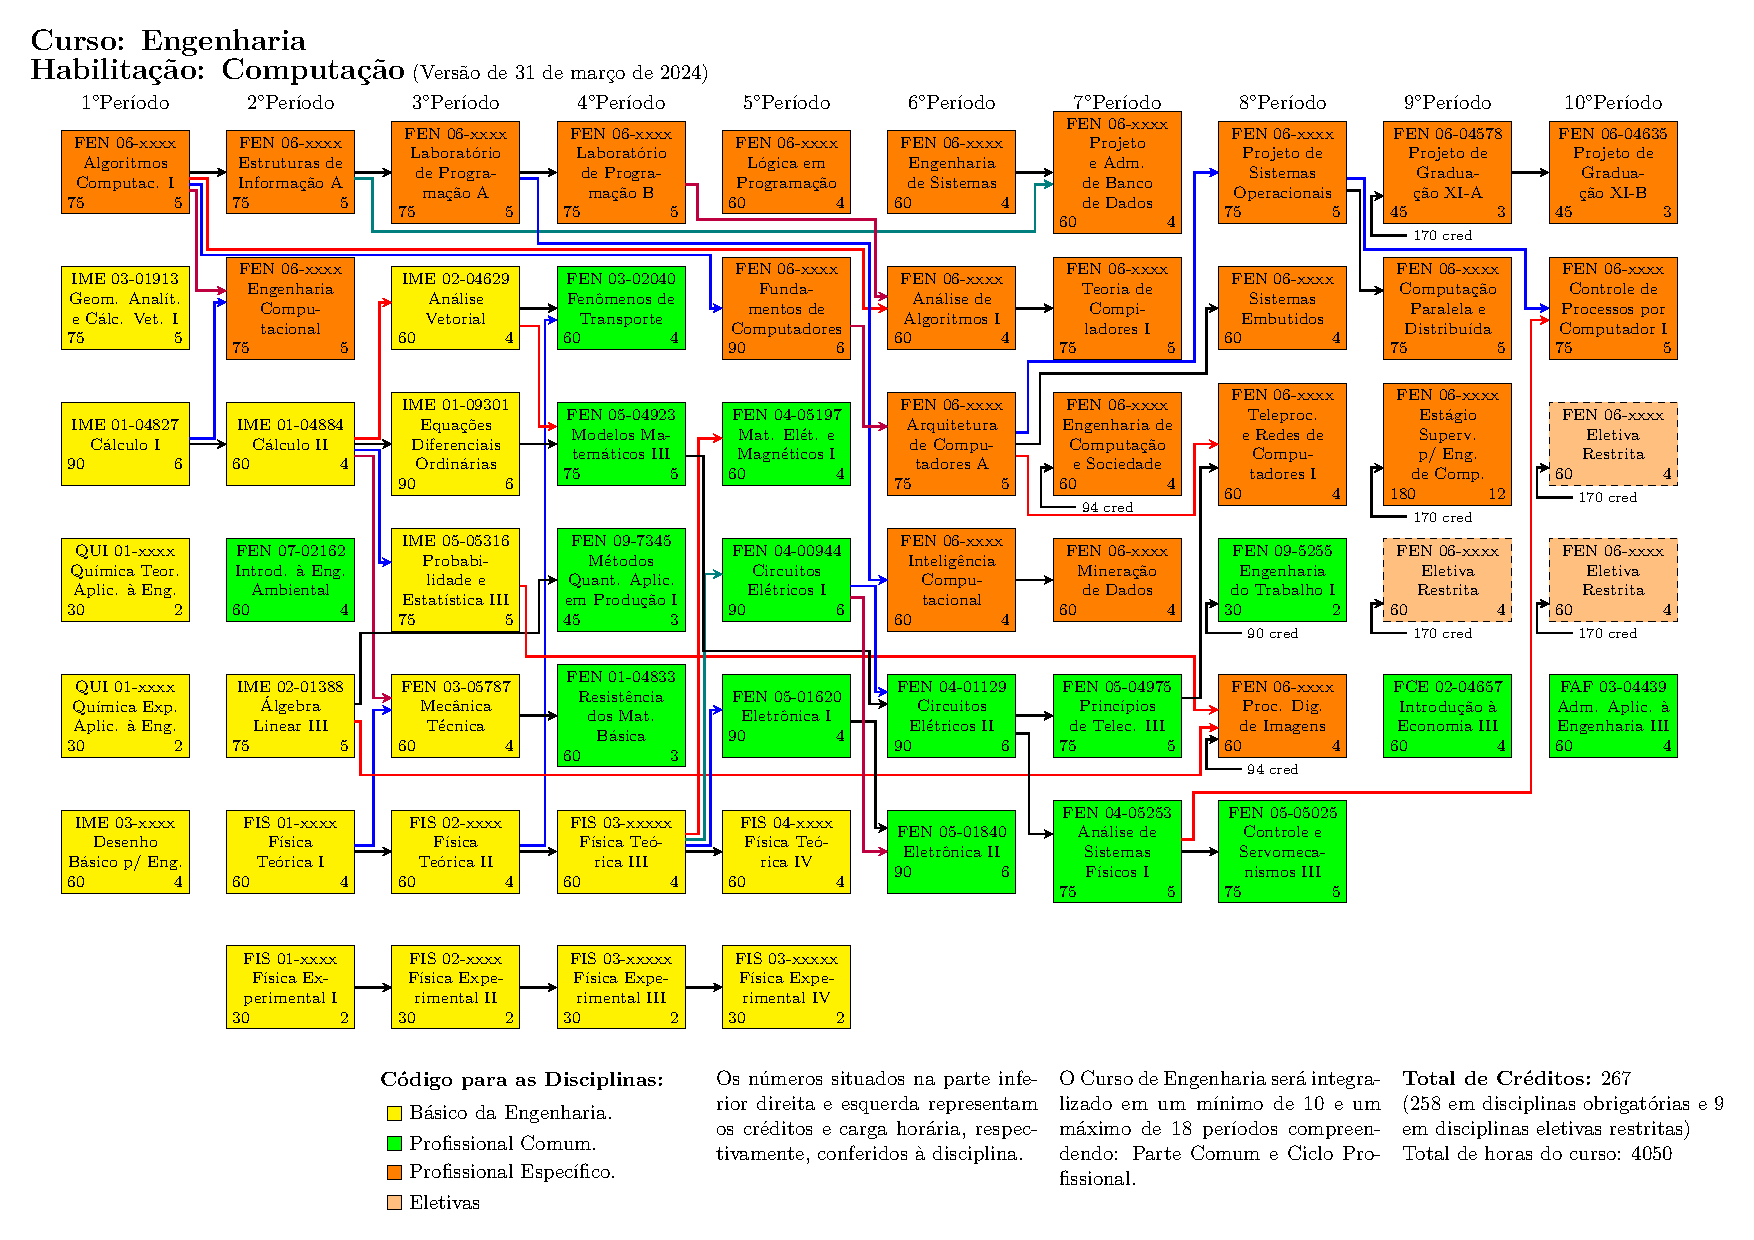
\includepdf[pages=-,angle=90]{fluxogramaEngenhariaComputacao.pdf}
\chapter{Ementas do Curso de Engenharia de Computação}
\label{ementas}
\includepdf[pages=-,addtotoc={1,section,1,{\Adm},},pagecommand={\thispagestyle{fancy}}]{ementasExternas/administracao_financeira_de_projeto.pdf}
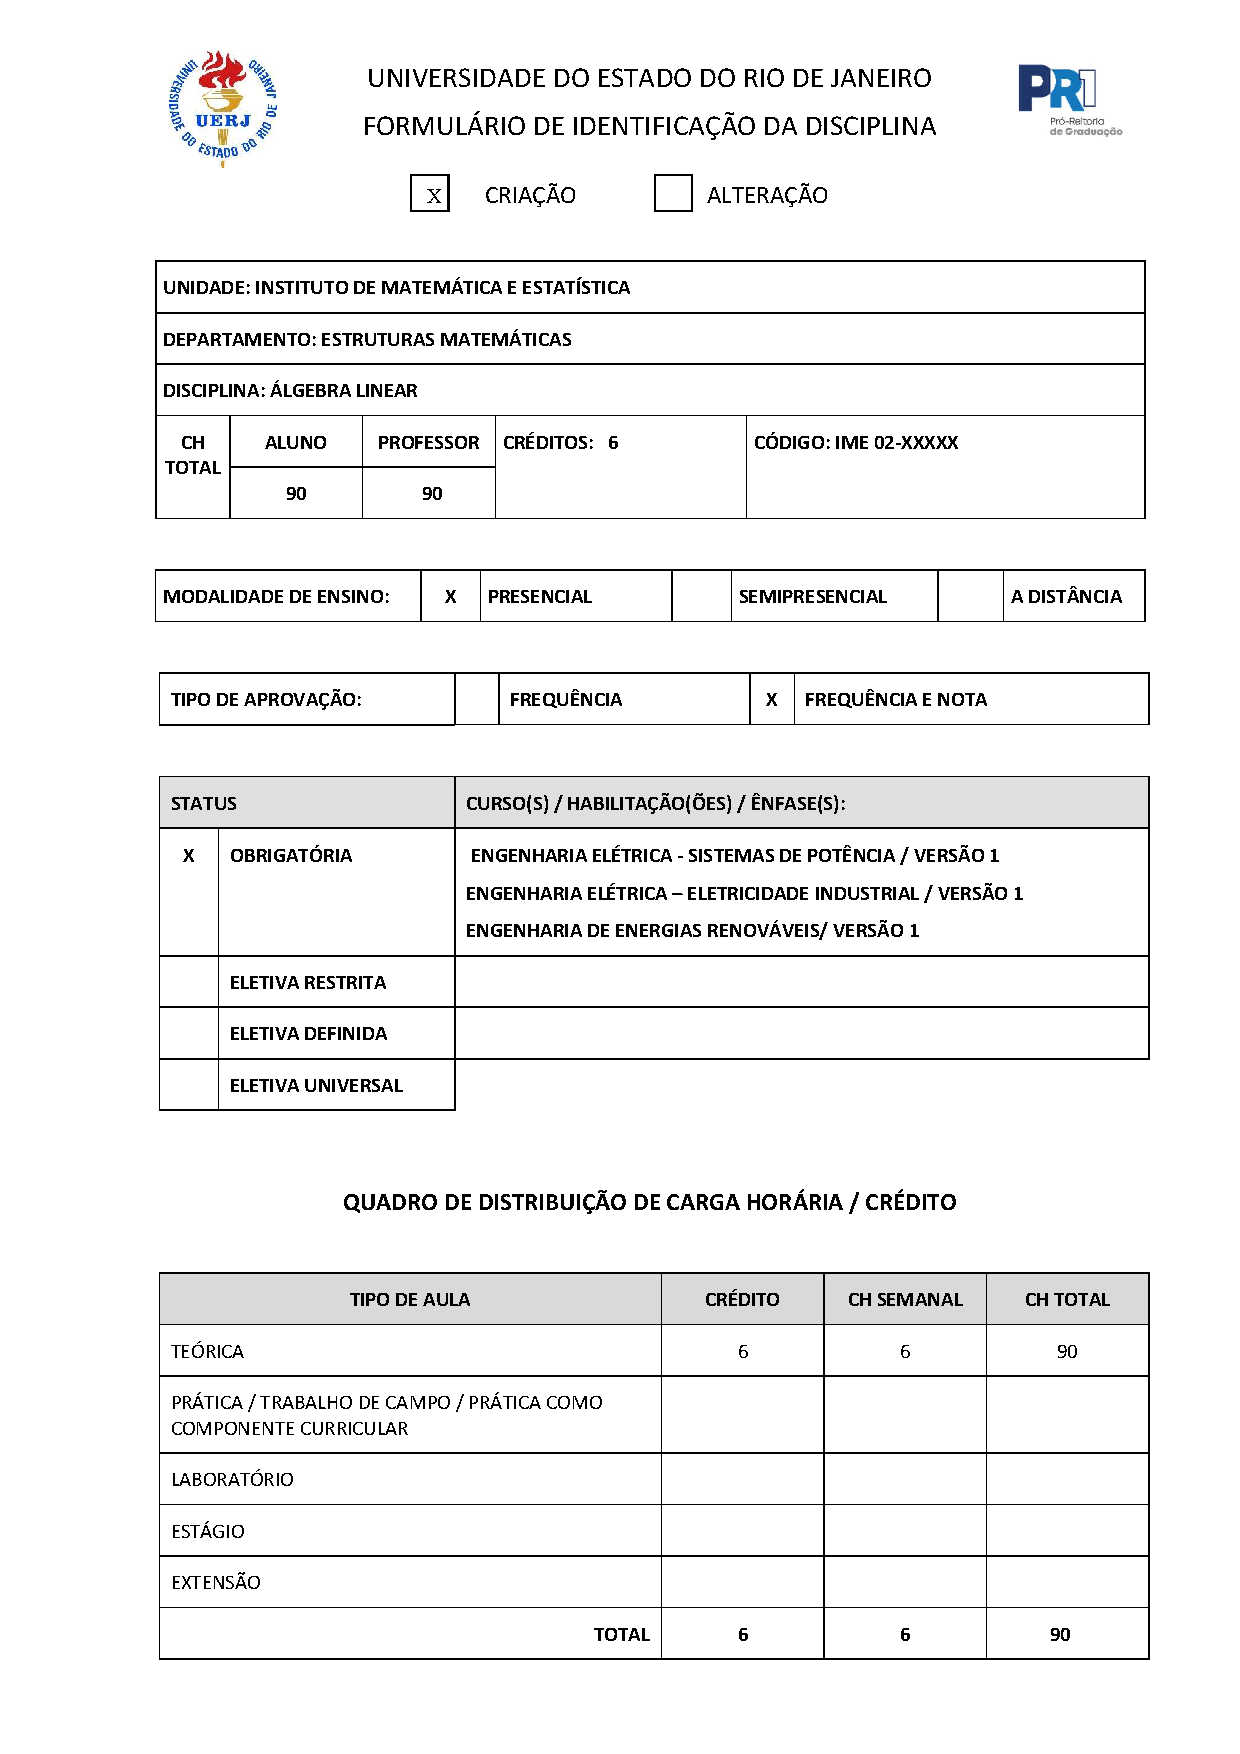
\includepdf[pages=-,addtotoc={1,section,1,{\AlgLin},},pagecommand={\thispagestyle{fancy}}]{ementasExternas/Algebra_Linear_90hs.pdf}
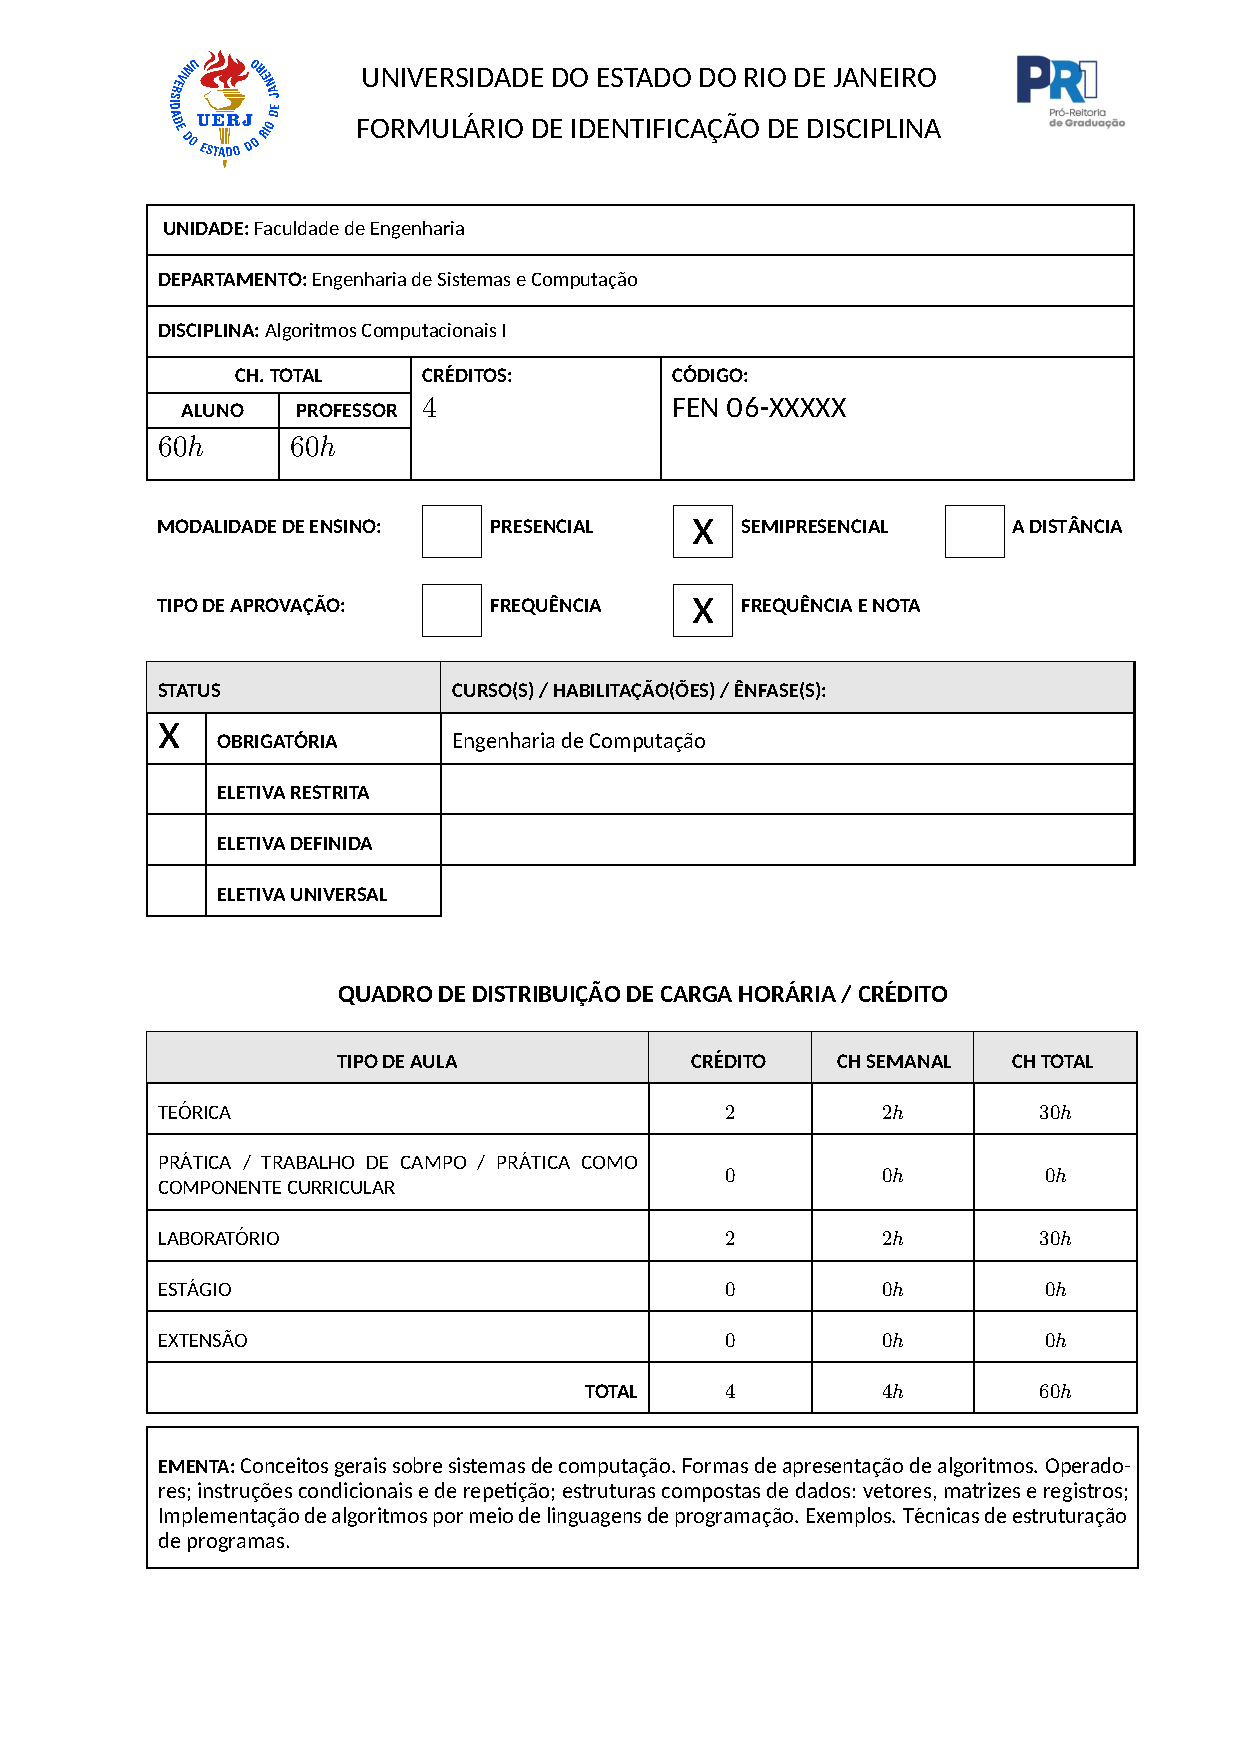
\includepdf[pages=-,addtotoc={1,section,1,{\AlgComp},},pagecommand={\thispagestyle{fancy}}]{ementas/AlgoritmosComputacionais.pdf}
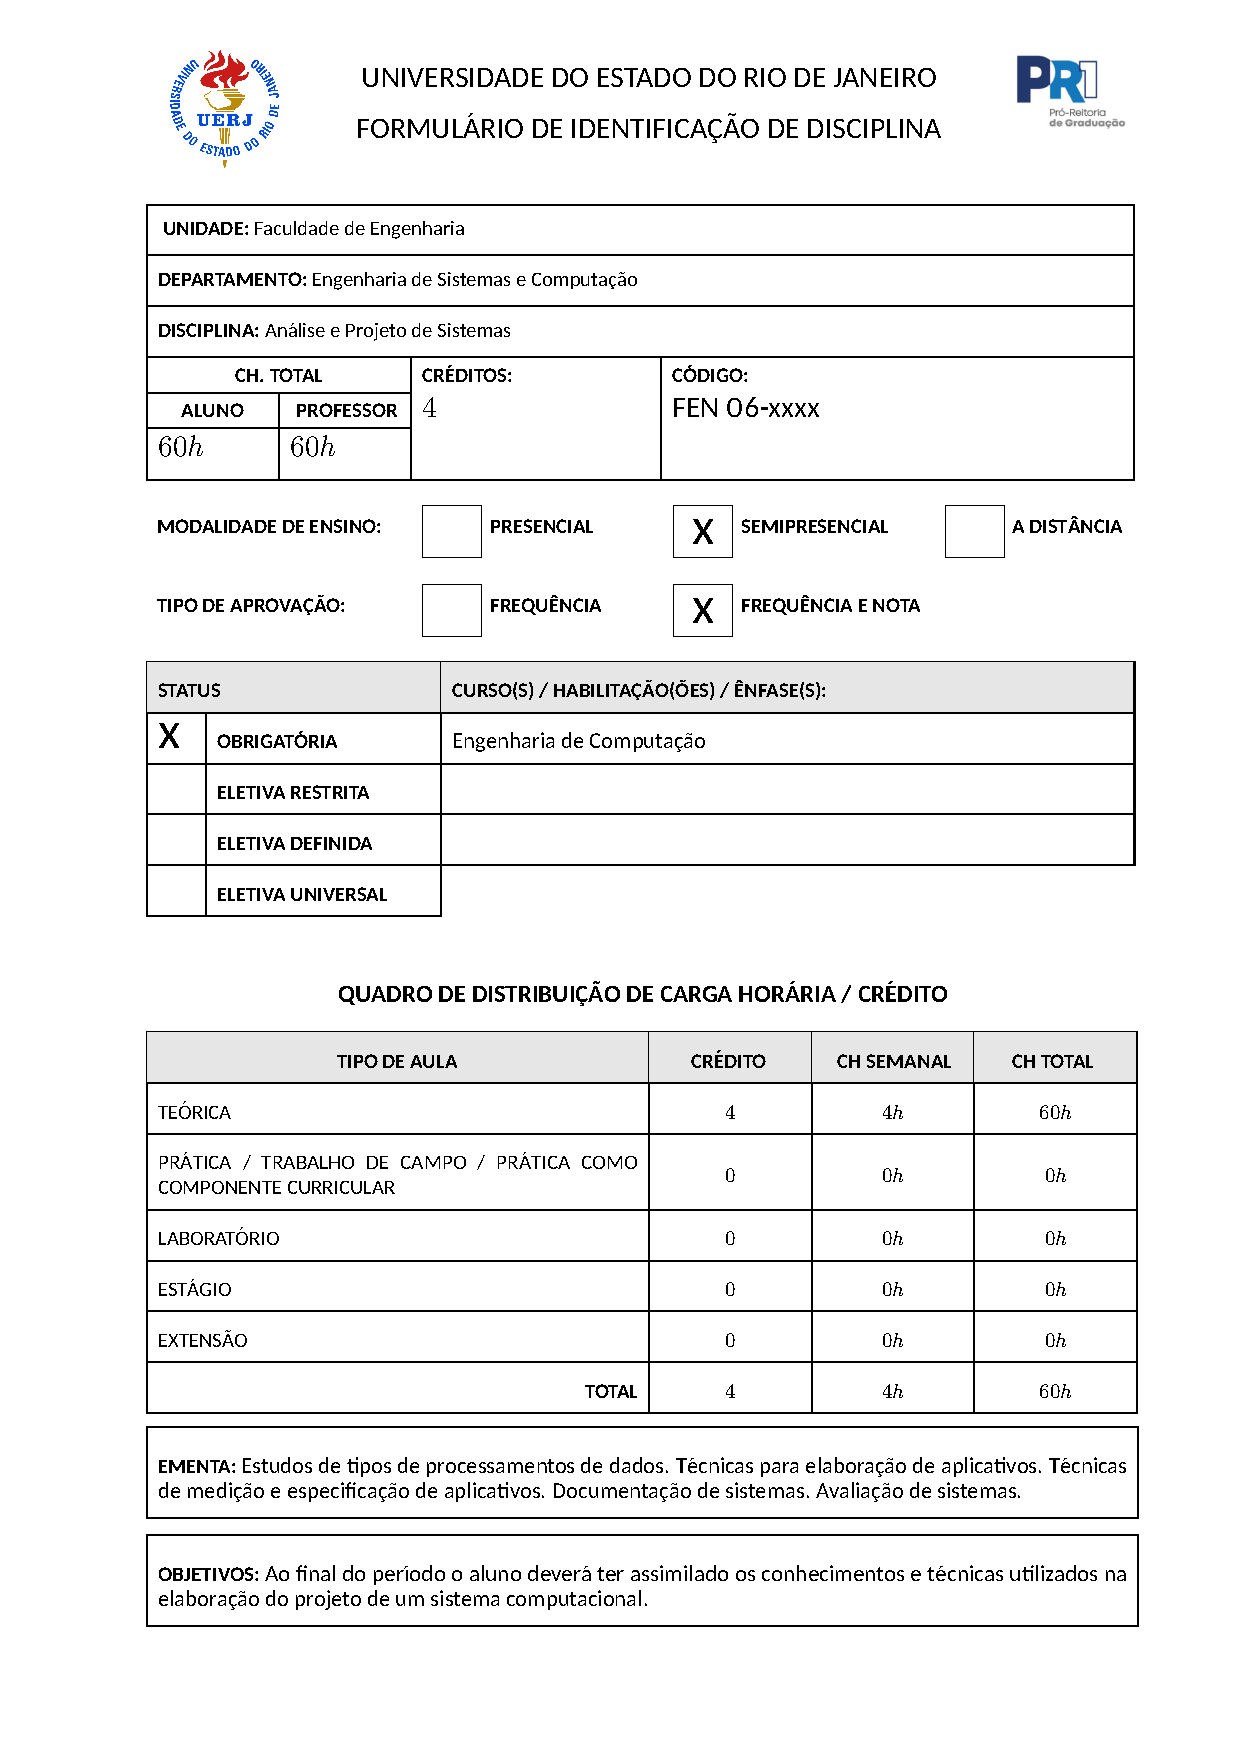
\includepdf[pages=-,addtotoc={1,section,1,{\AnaProjSist},},pagecommand={\thispagestyle{fancy}}]{ementas/analise_e_projeto_de_sistemas.pdf}
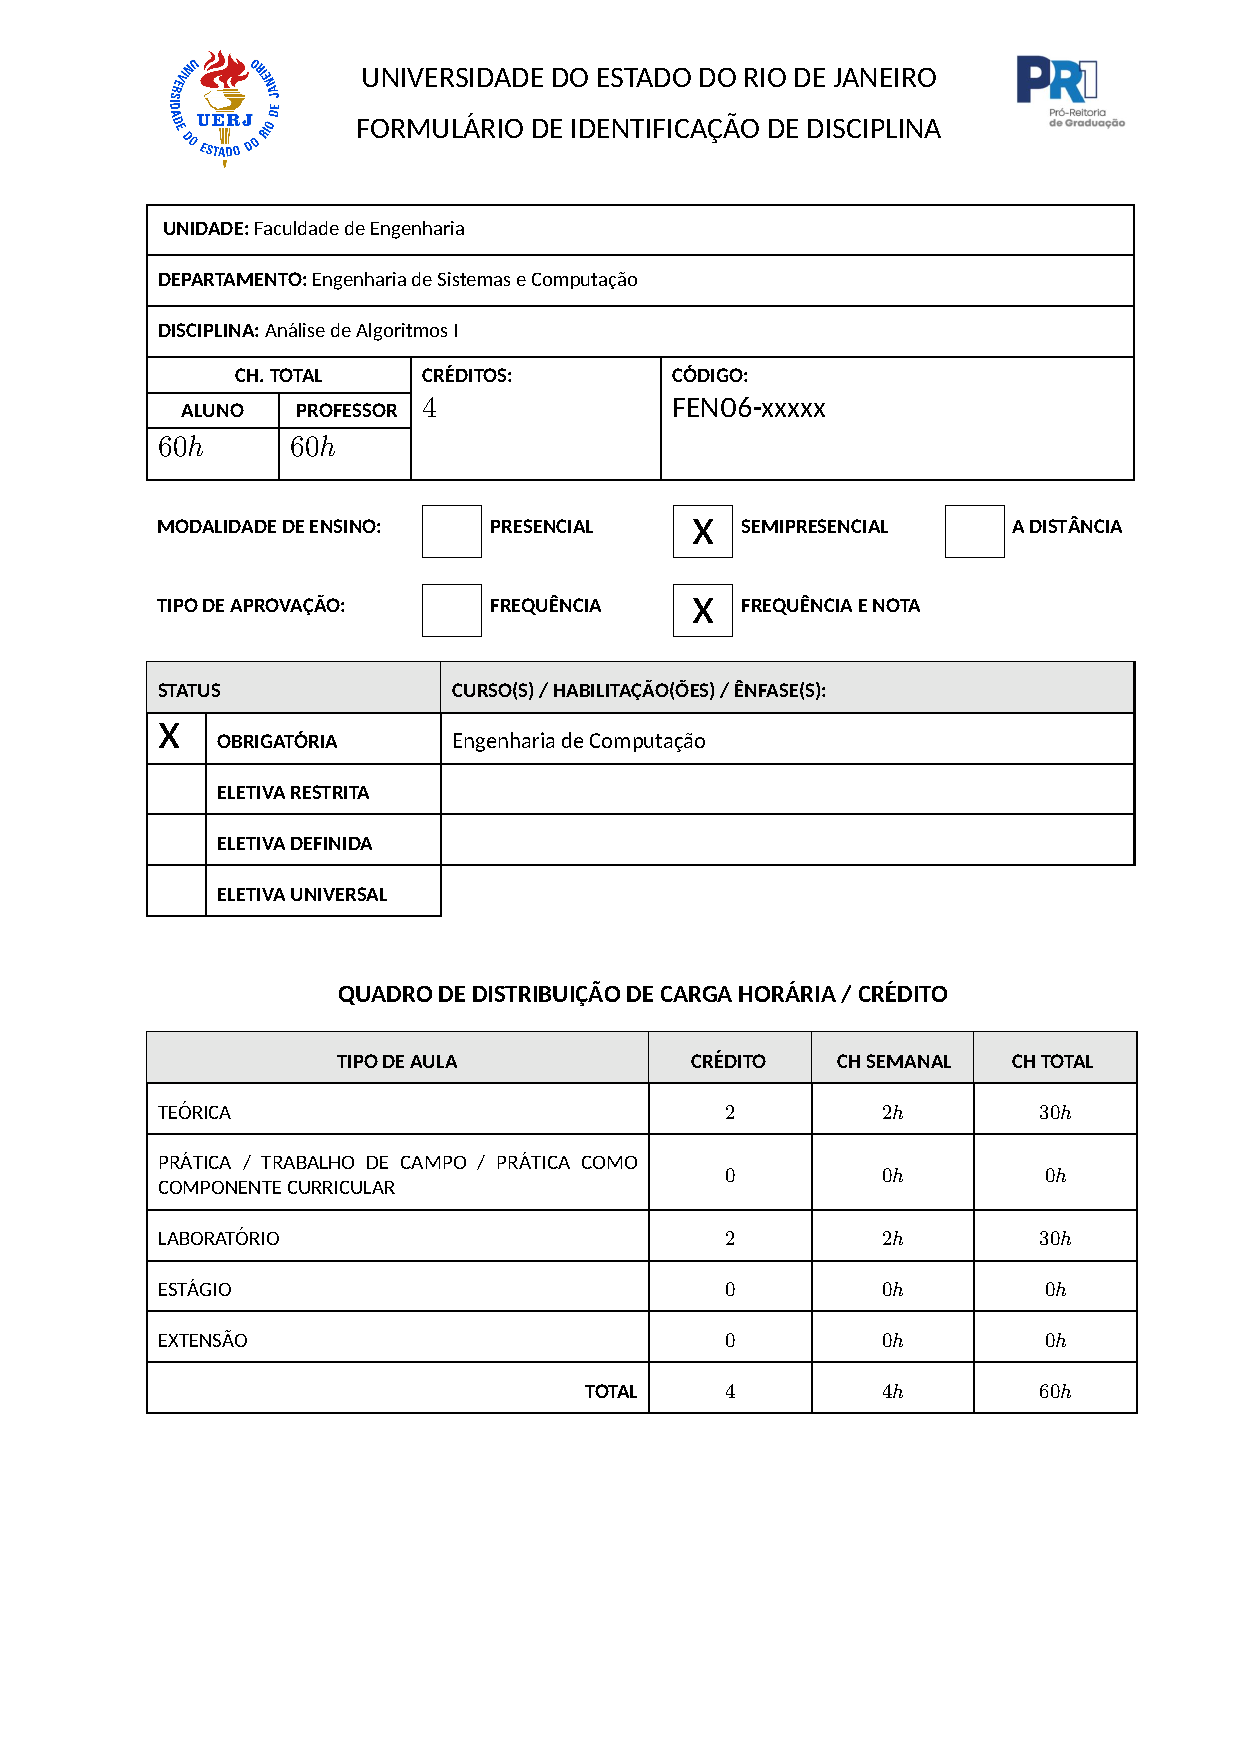
\includepdf[pages=-,addtotoc={1,section,1,{\AnAlg},},pagecommand={\thispagestyle{fancy}}]{ementas/AnaliseDeAlgoritmos.pdf}
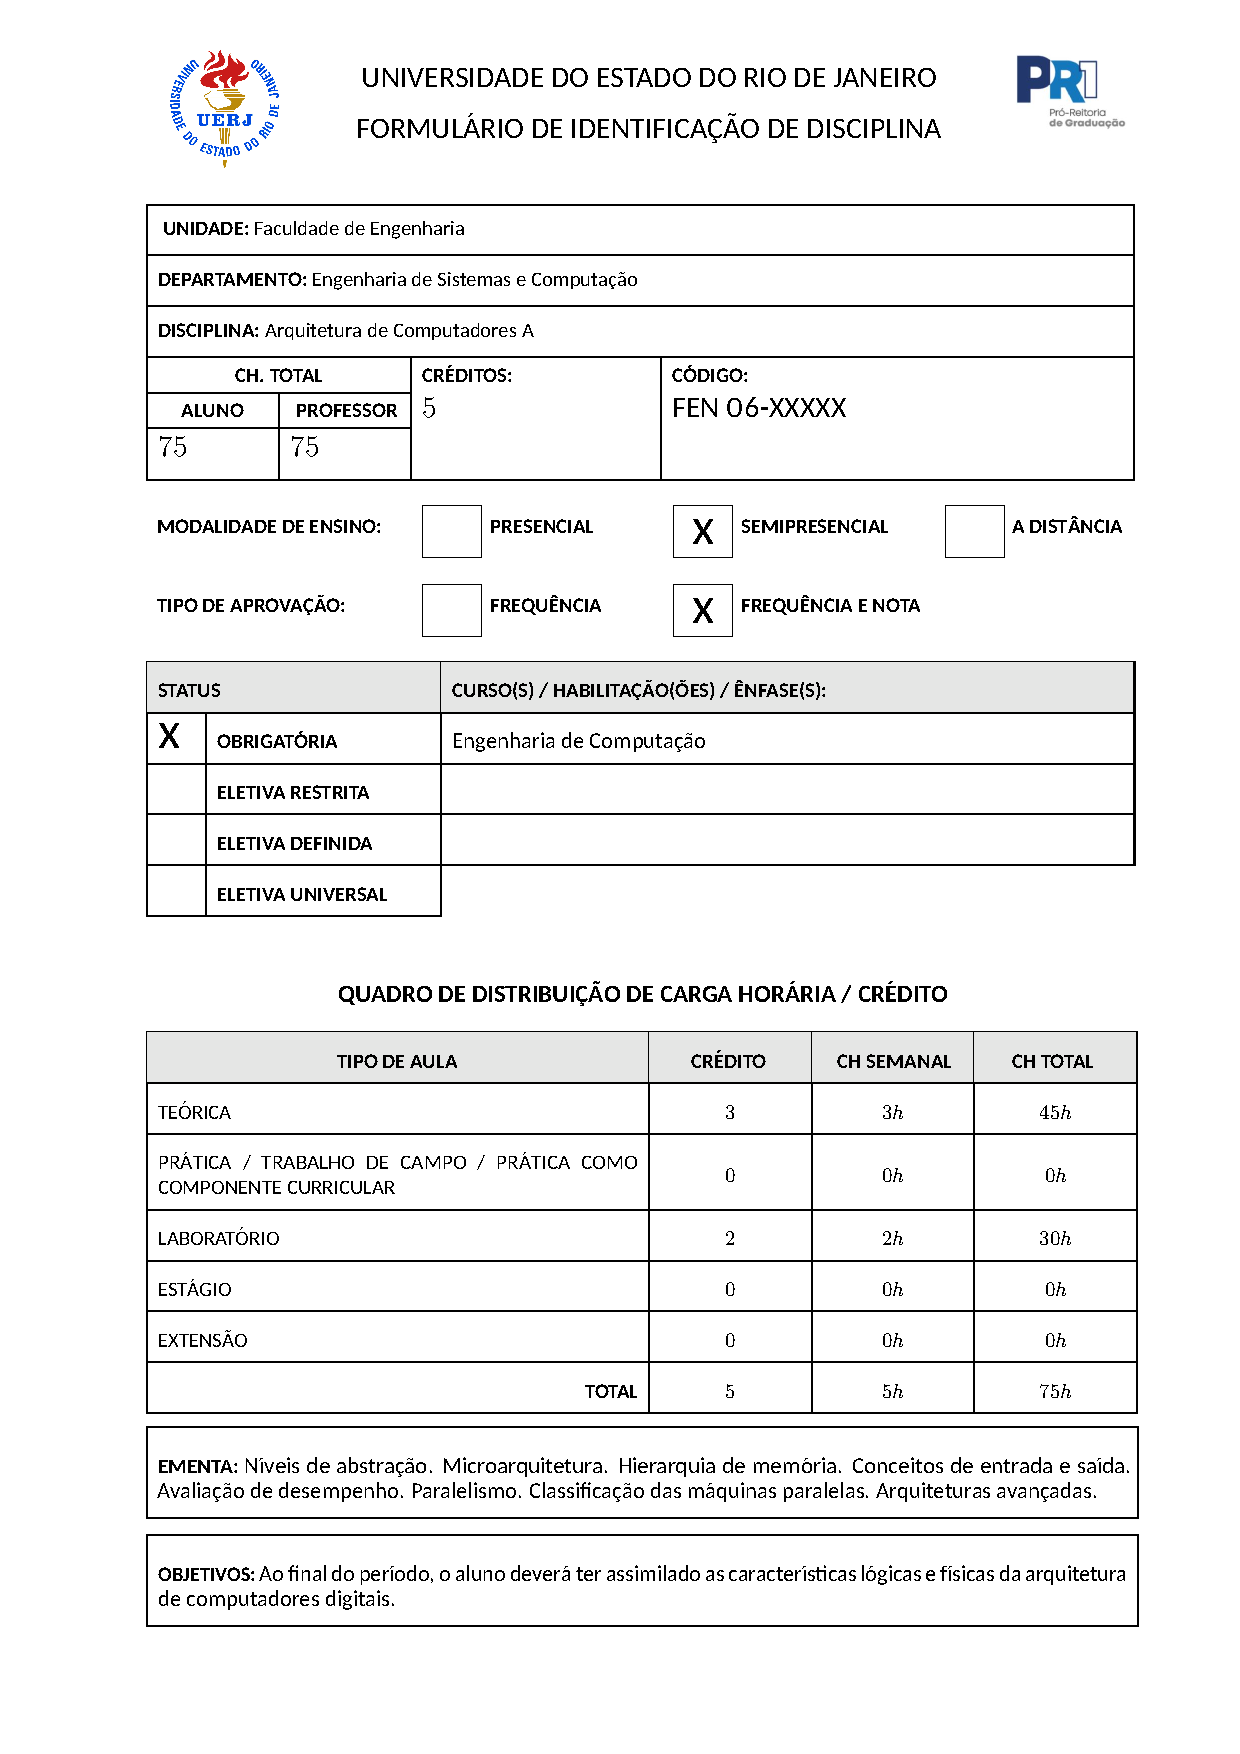
\includepdf[pages=-,addtotoc={1,section,1,{\ArqComp},},pagecommand={\thispagestyle{fancy}}]{ementas/ArquiteturaDeComputadores.pdf}
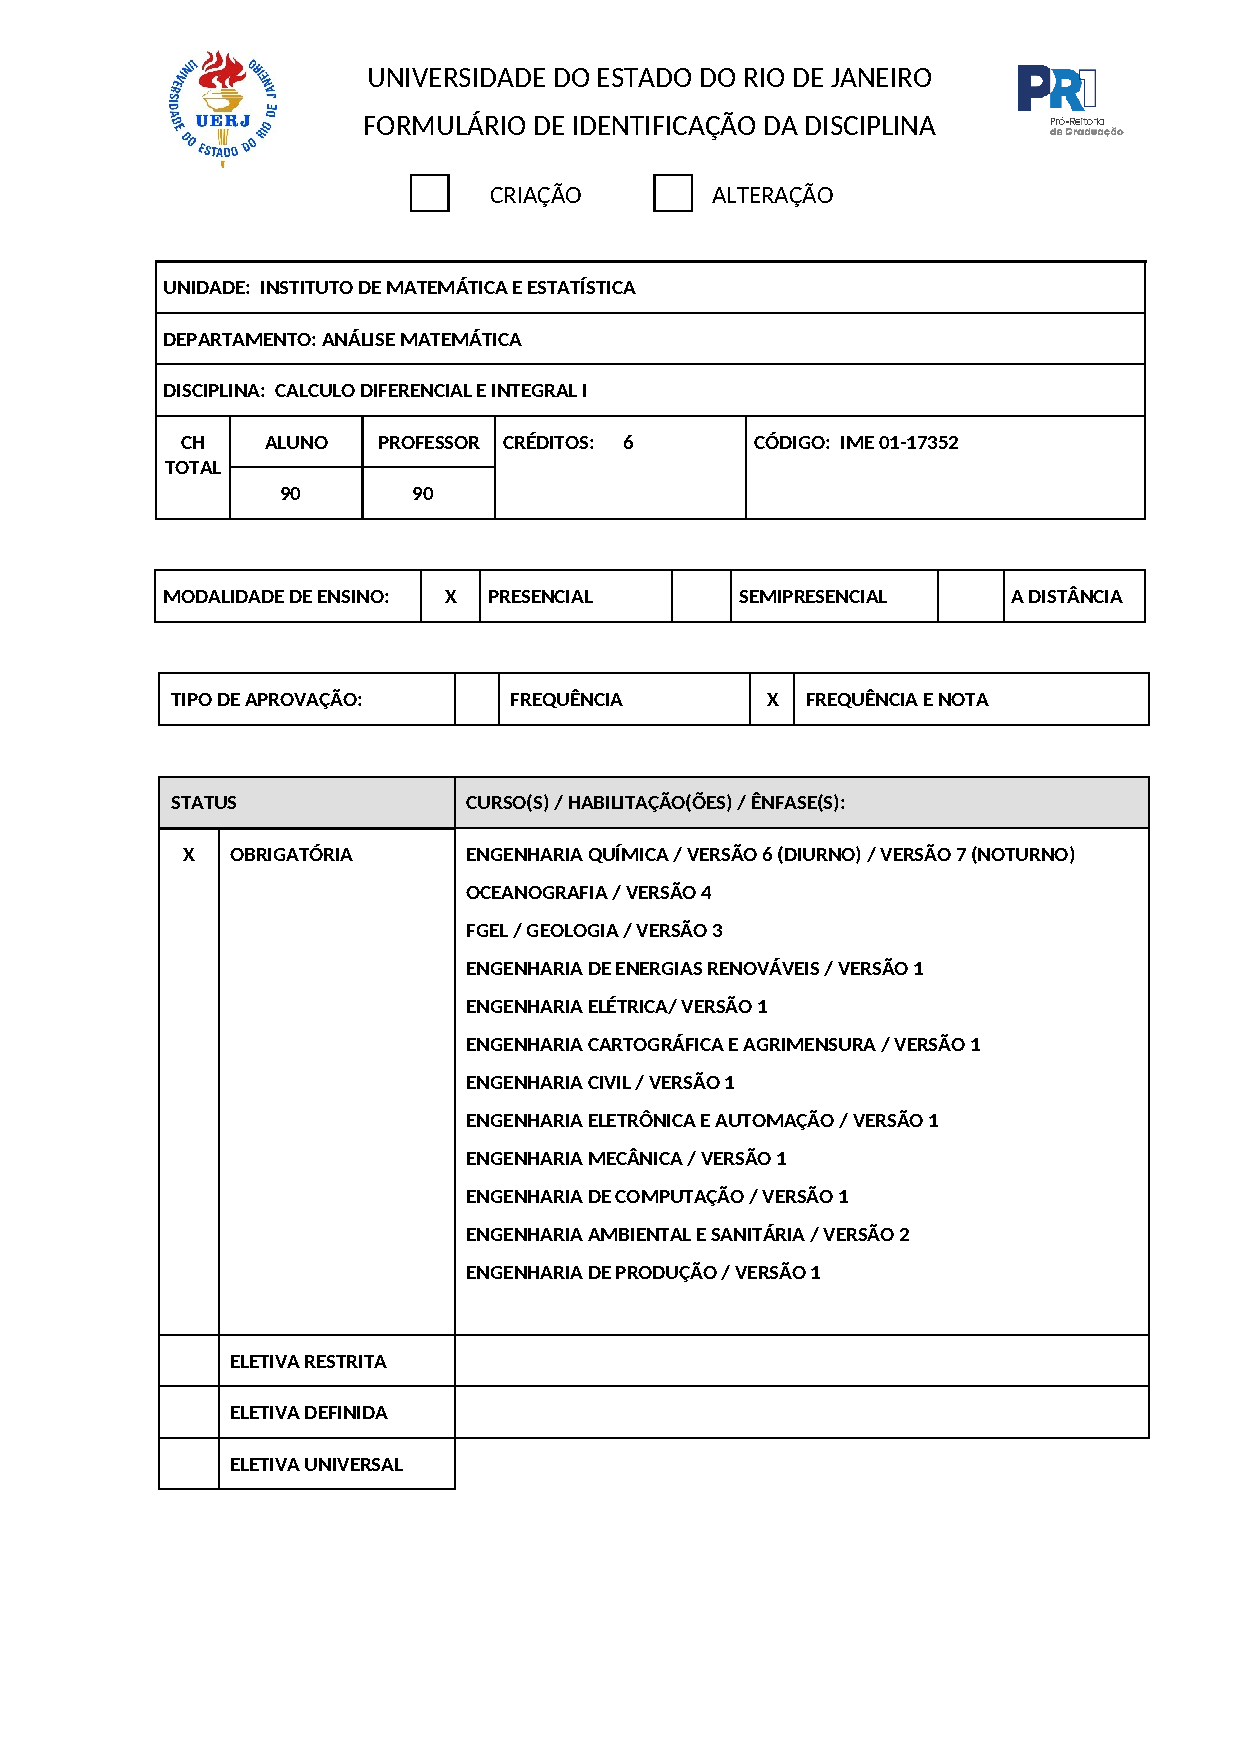
\includepdf[pages=-,addtotoc={1,section,1,{\CalcI},},pagecommand={\thispagestyle{fancy}}]{ementasExternas/calculo_diferencial_e_integral_i.pdf}
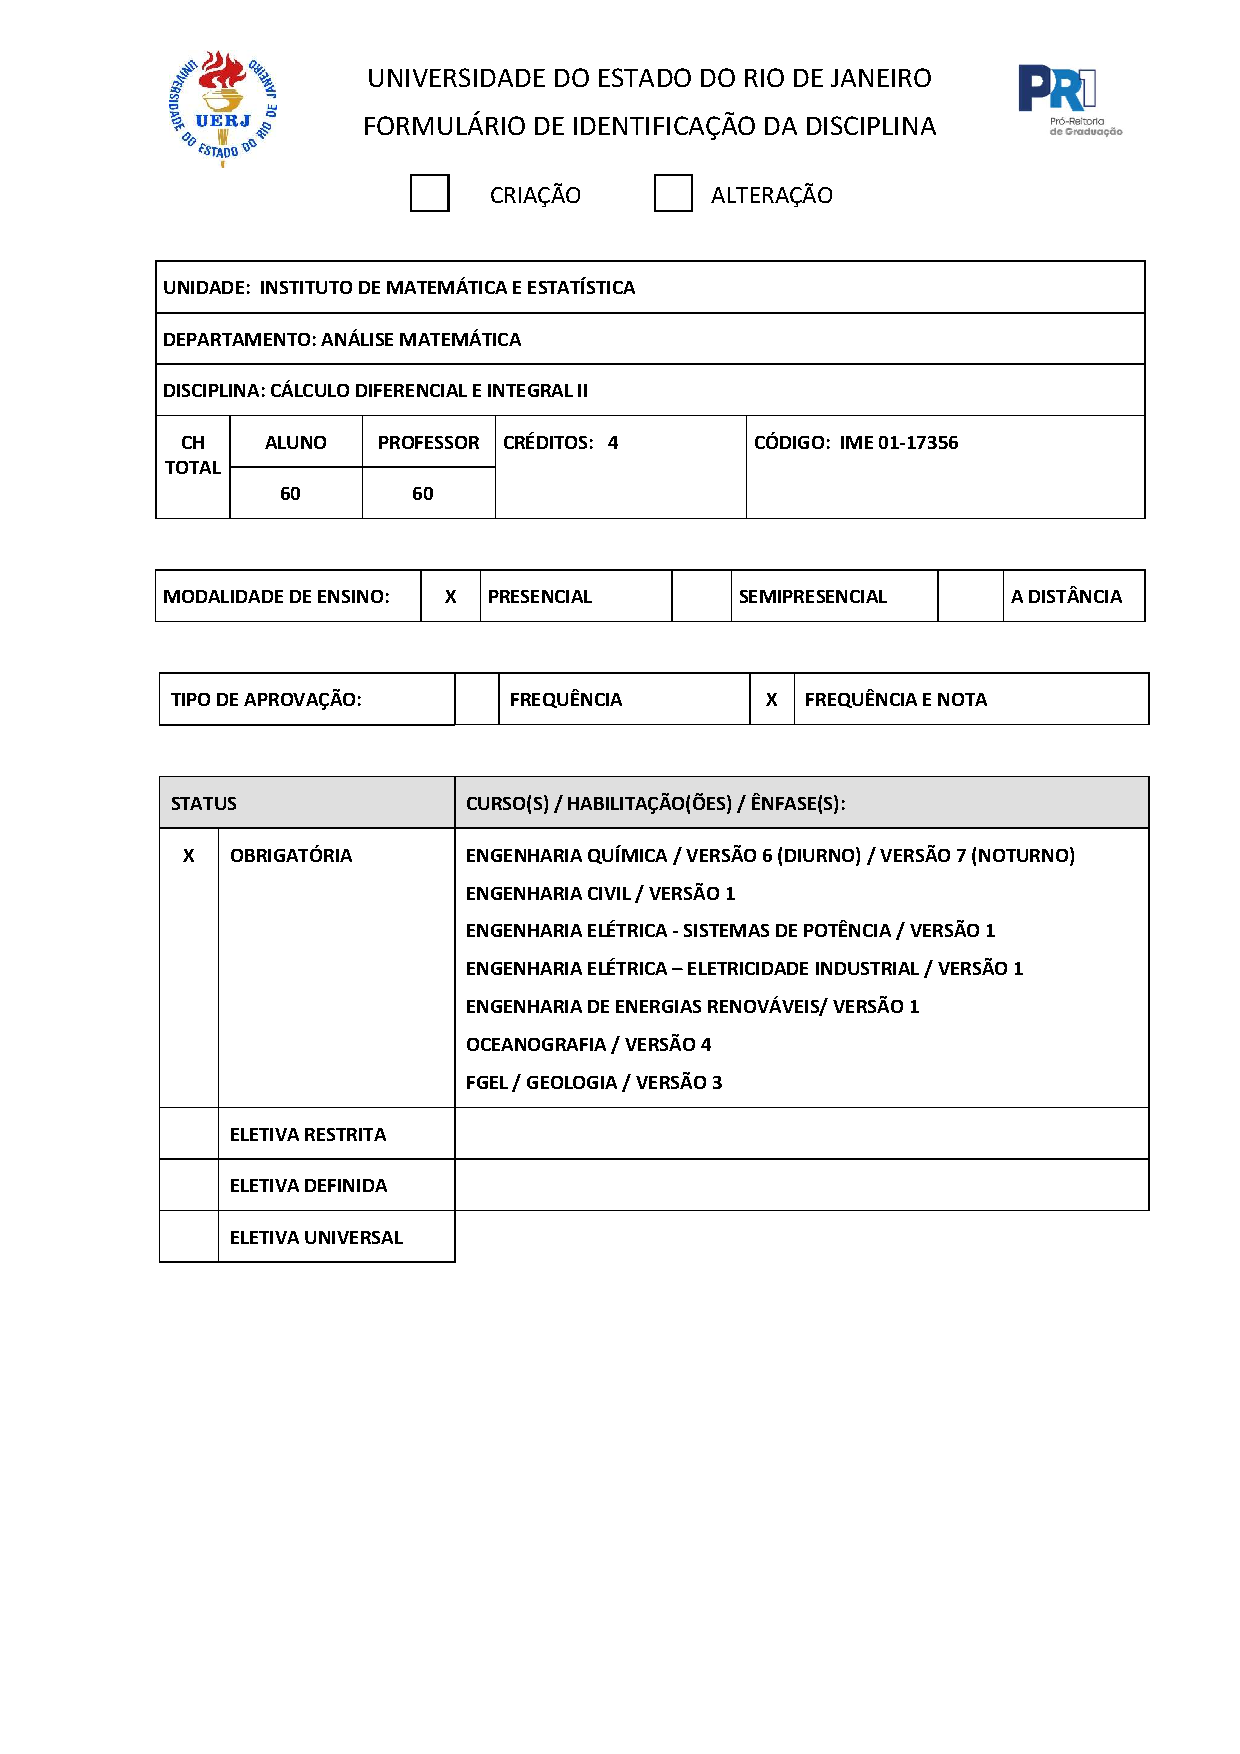
\includepdf[pages=-,addtotoc={1,section,1,{\CalcII},},pagecommand={\thispagestyle{fancy}}]{ementasExternas/calculo_diferencial_e_integral_ii.pdf}
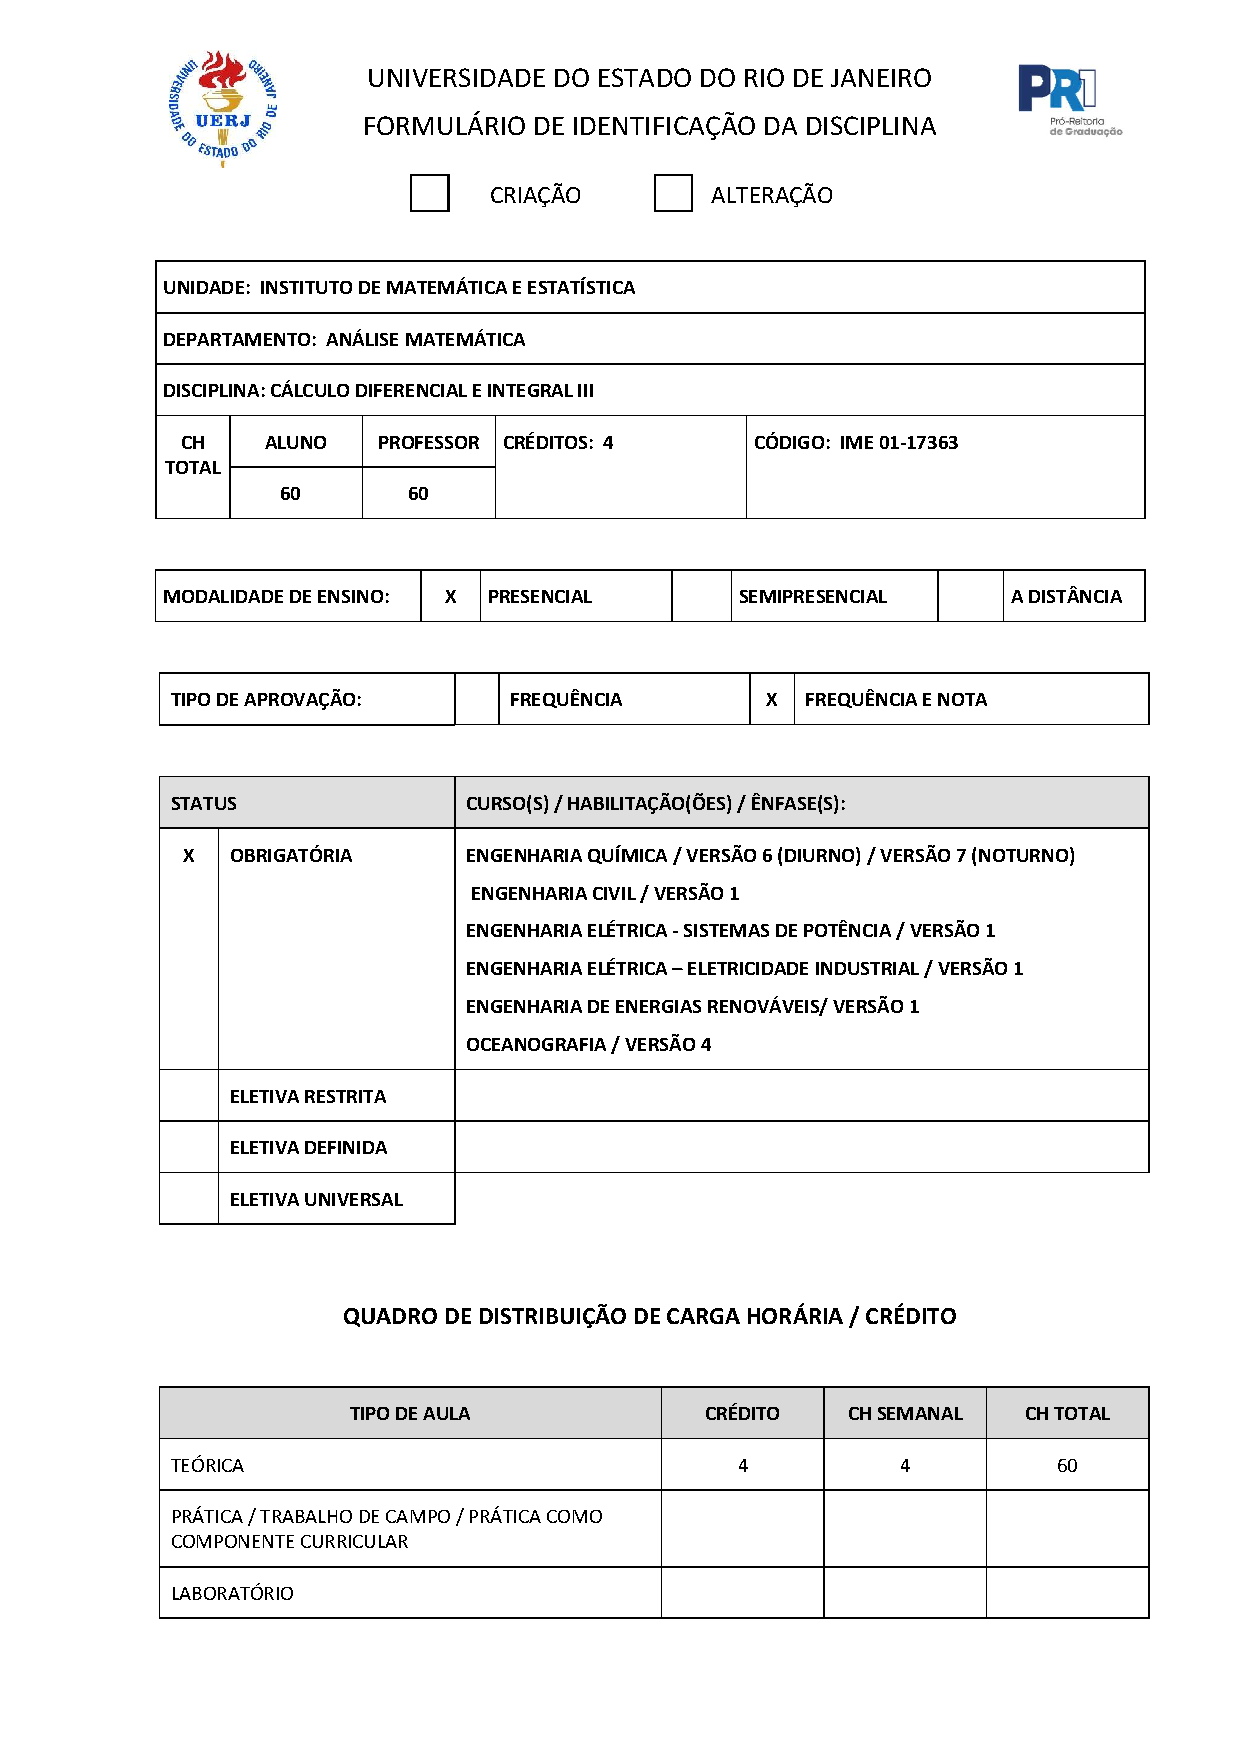
\includepdf[pages=-,addtotoc={1,section,1,{\CalcIII},},pagecommand={\thispagestyle{fancy}}]{ementasExternas/calculo_diferencial_e_integral_iii.pdf}
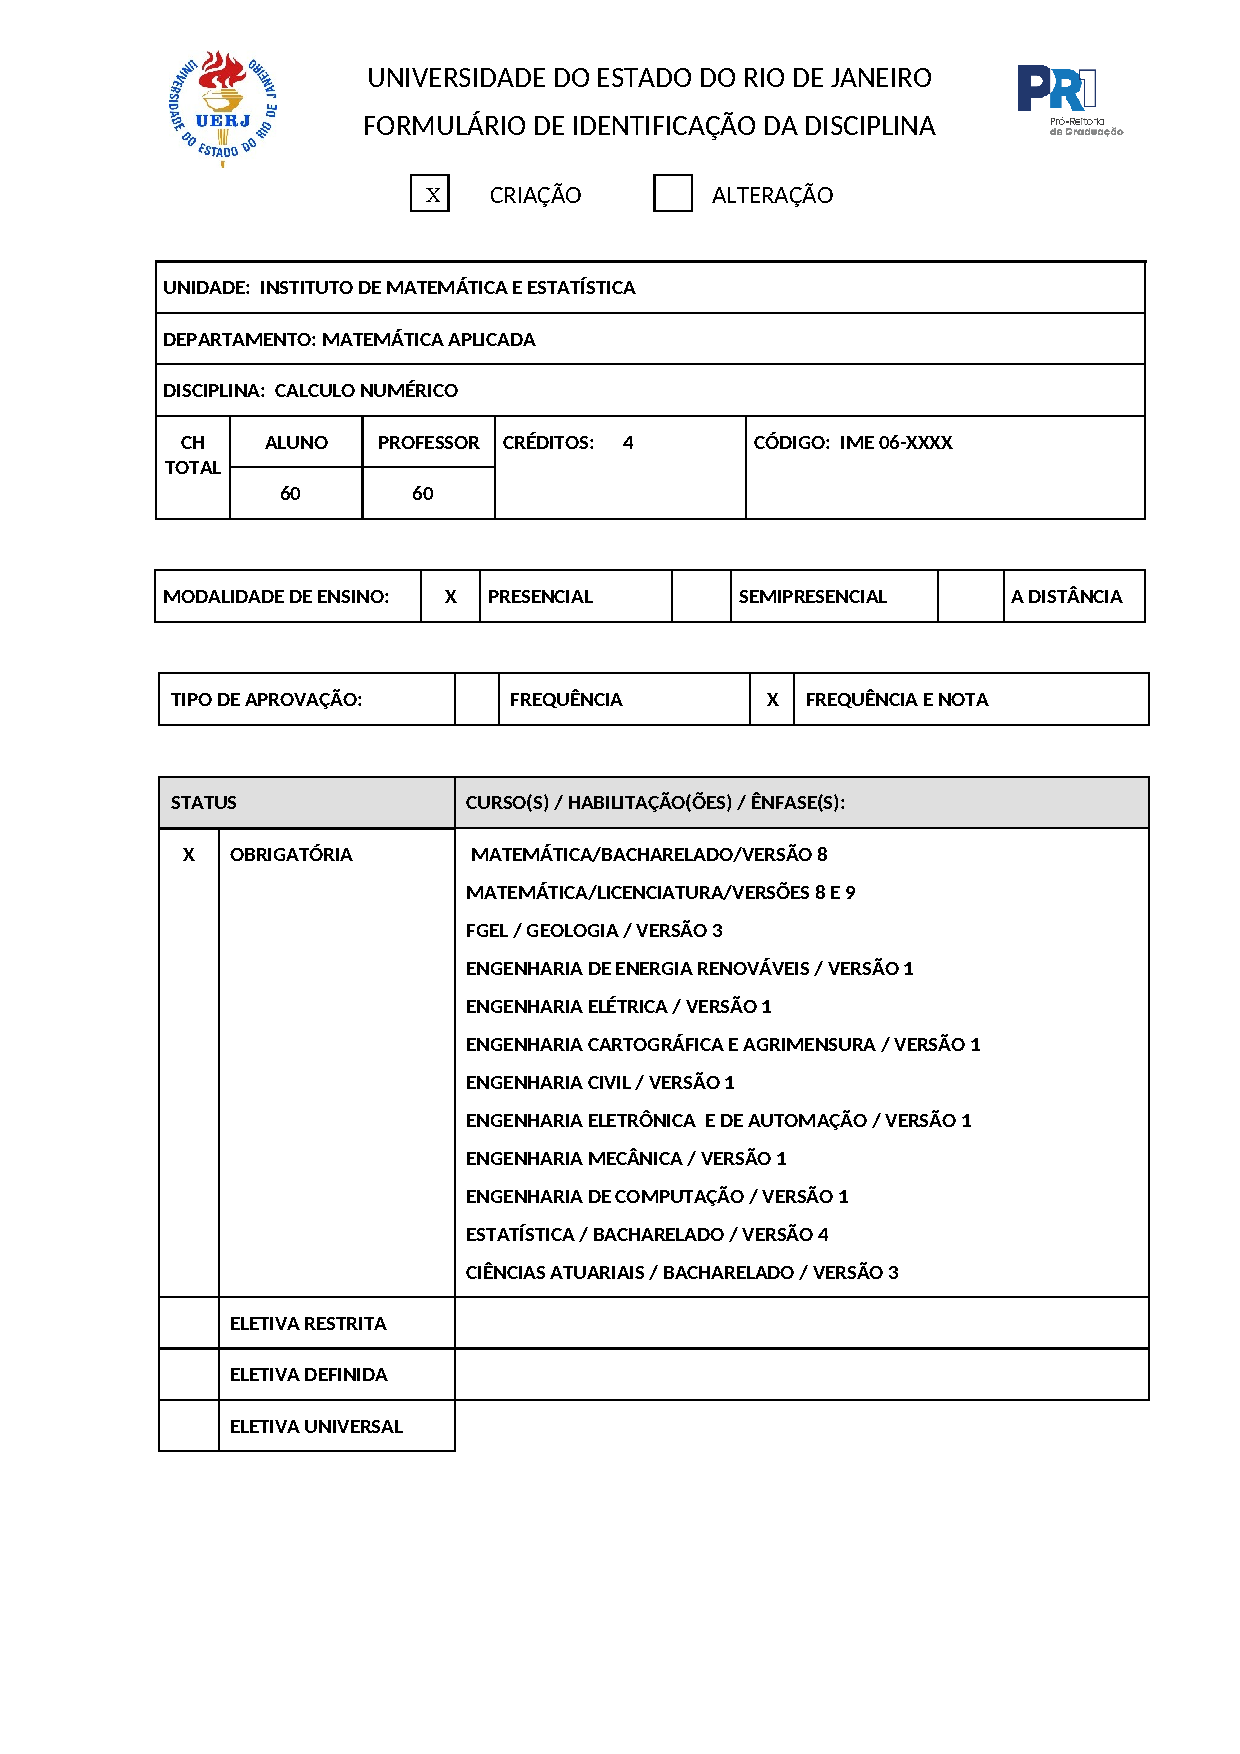
\includepdf[pages=-,addtotoc={1,section,1,{\CalcNum},},pagecommand={\thispagestyle{fancy}}]{ementasExternas/Calculo_Numerico.pdf}
\includepdf[pages=-,addtotoc={1,section,1,{\CalcNum},},pagecommand={\thispagestyle{fancy}}]{ementasExternas/circuitos_eletronicos_i.pdf}% Circuitos Eletrônicos I
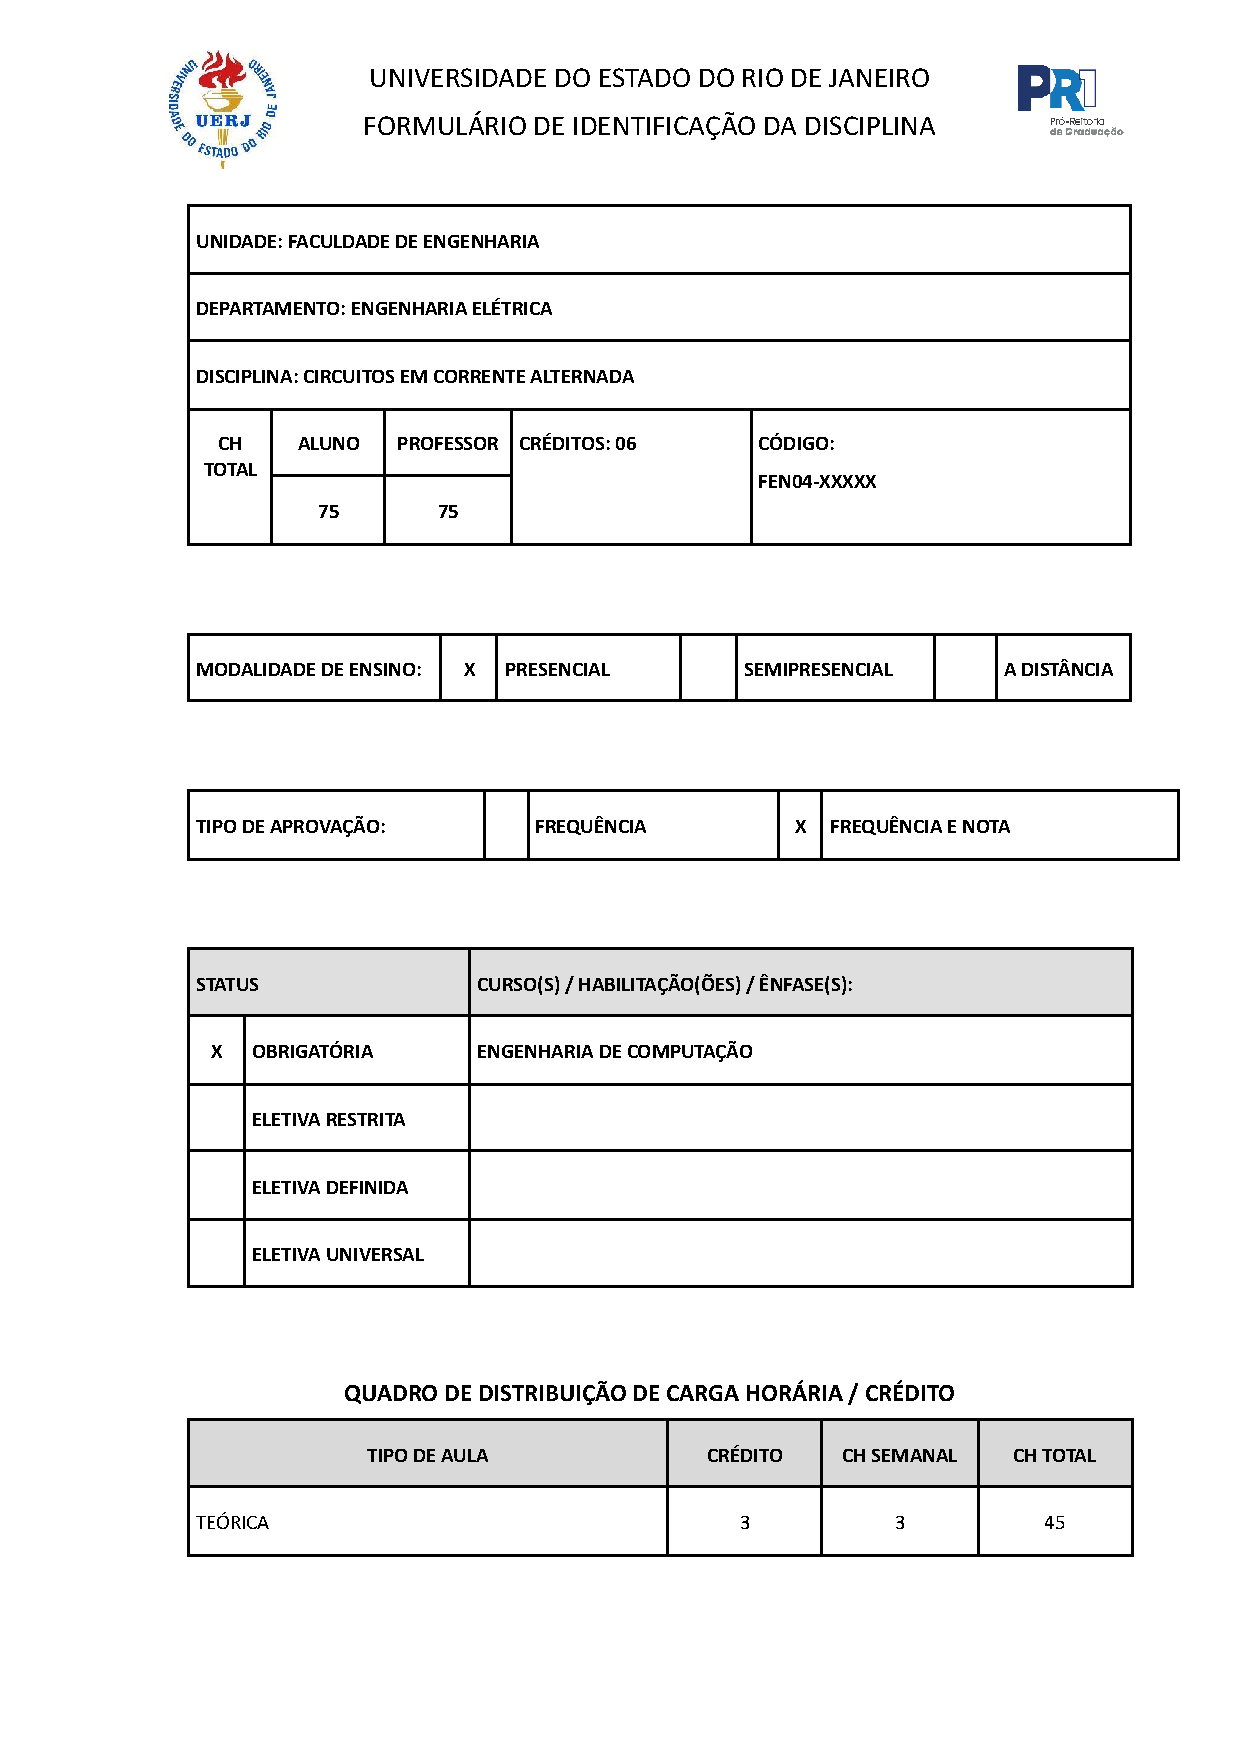
\includepdf[pages=-,addtotoc={1,section,1,{\CCA},},pagecommand={\thispagestyle{fancy}}]{ementasExternas/Eletrica/CircuitosemCorrenteAlternada.pdf}
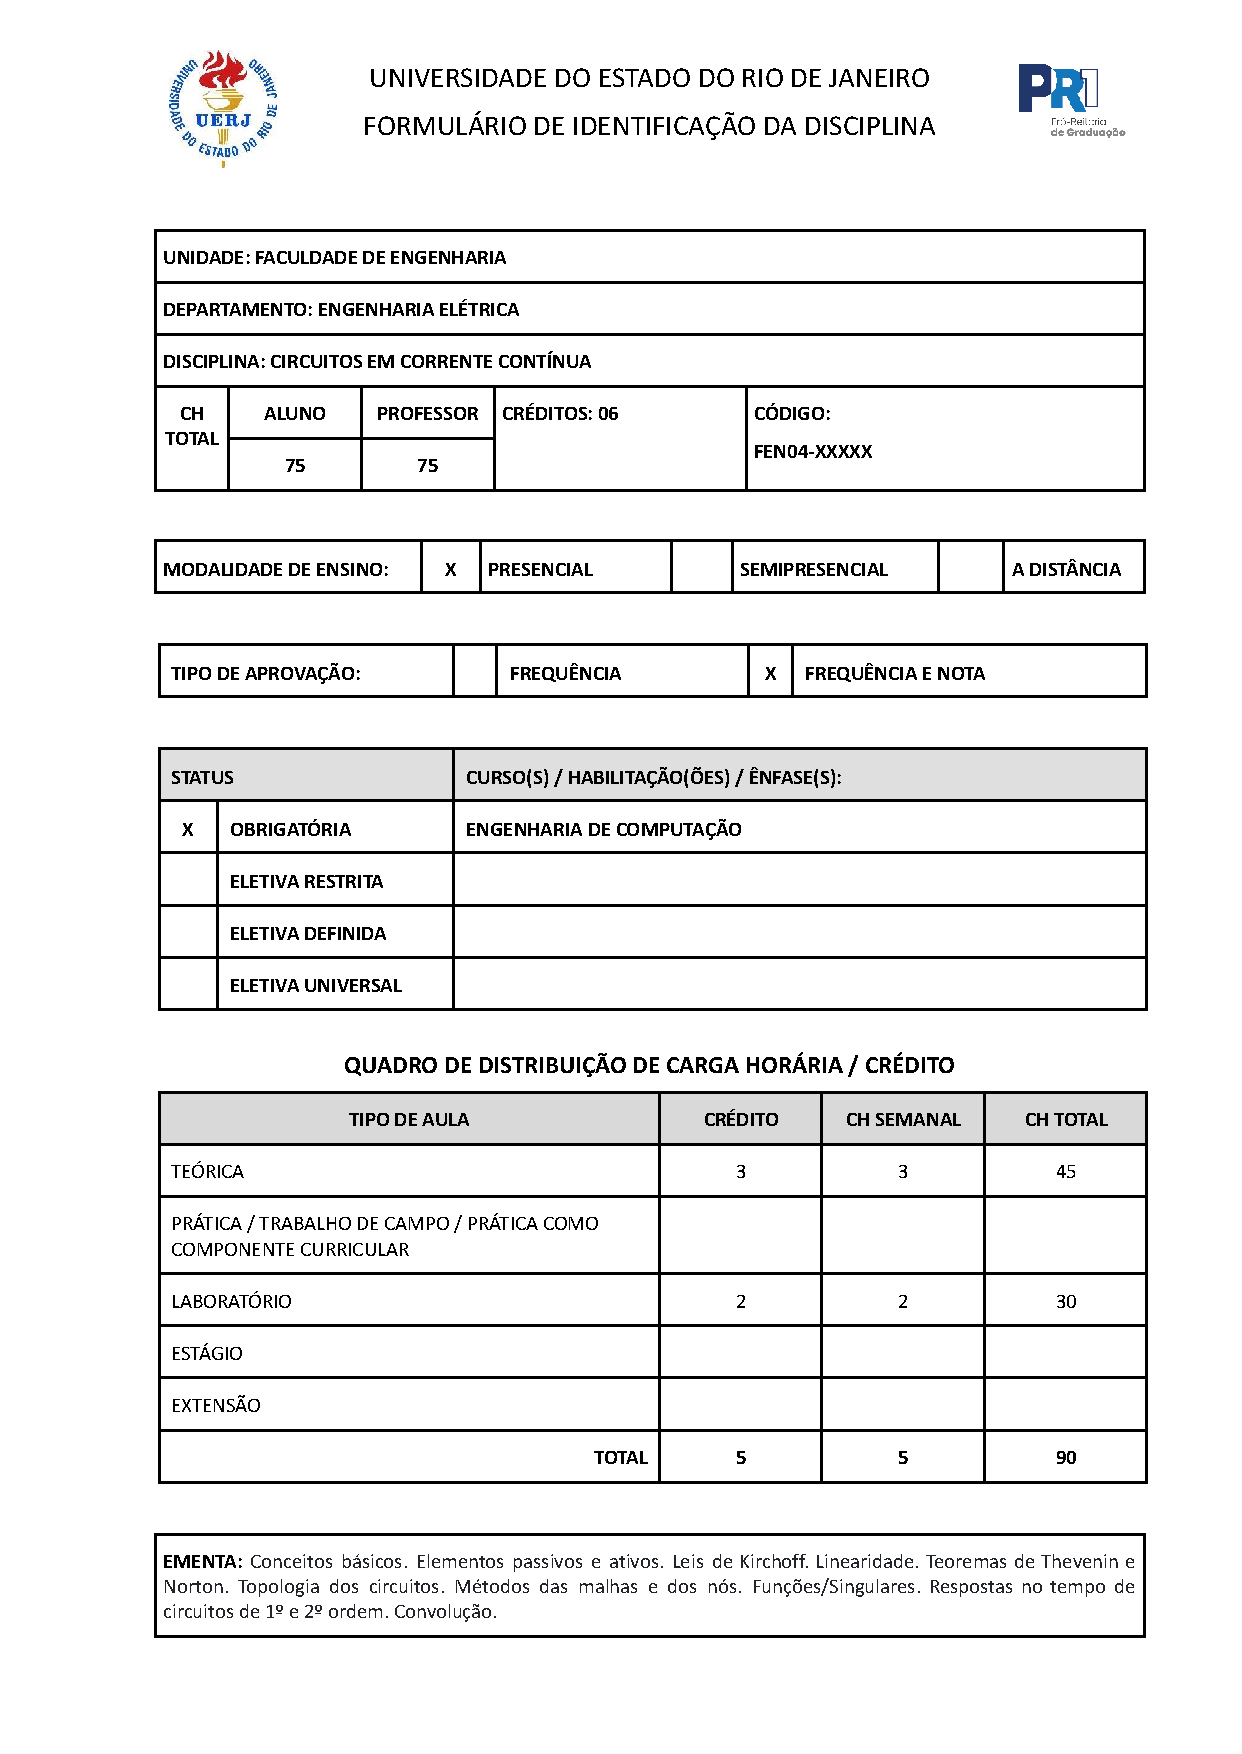
\includepdf[pages=-,addtotoc={1,section,1,{\CCC},},pagecommand={\thispagestyle{fancy}}]{ementasExternas/Eletrica/CircuitosemCorrenteContinua.pdf}
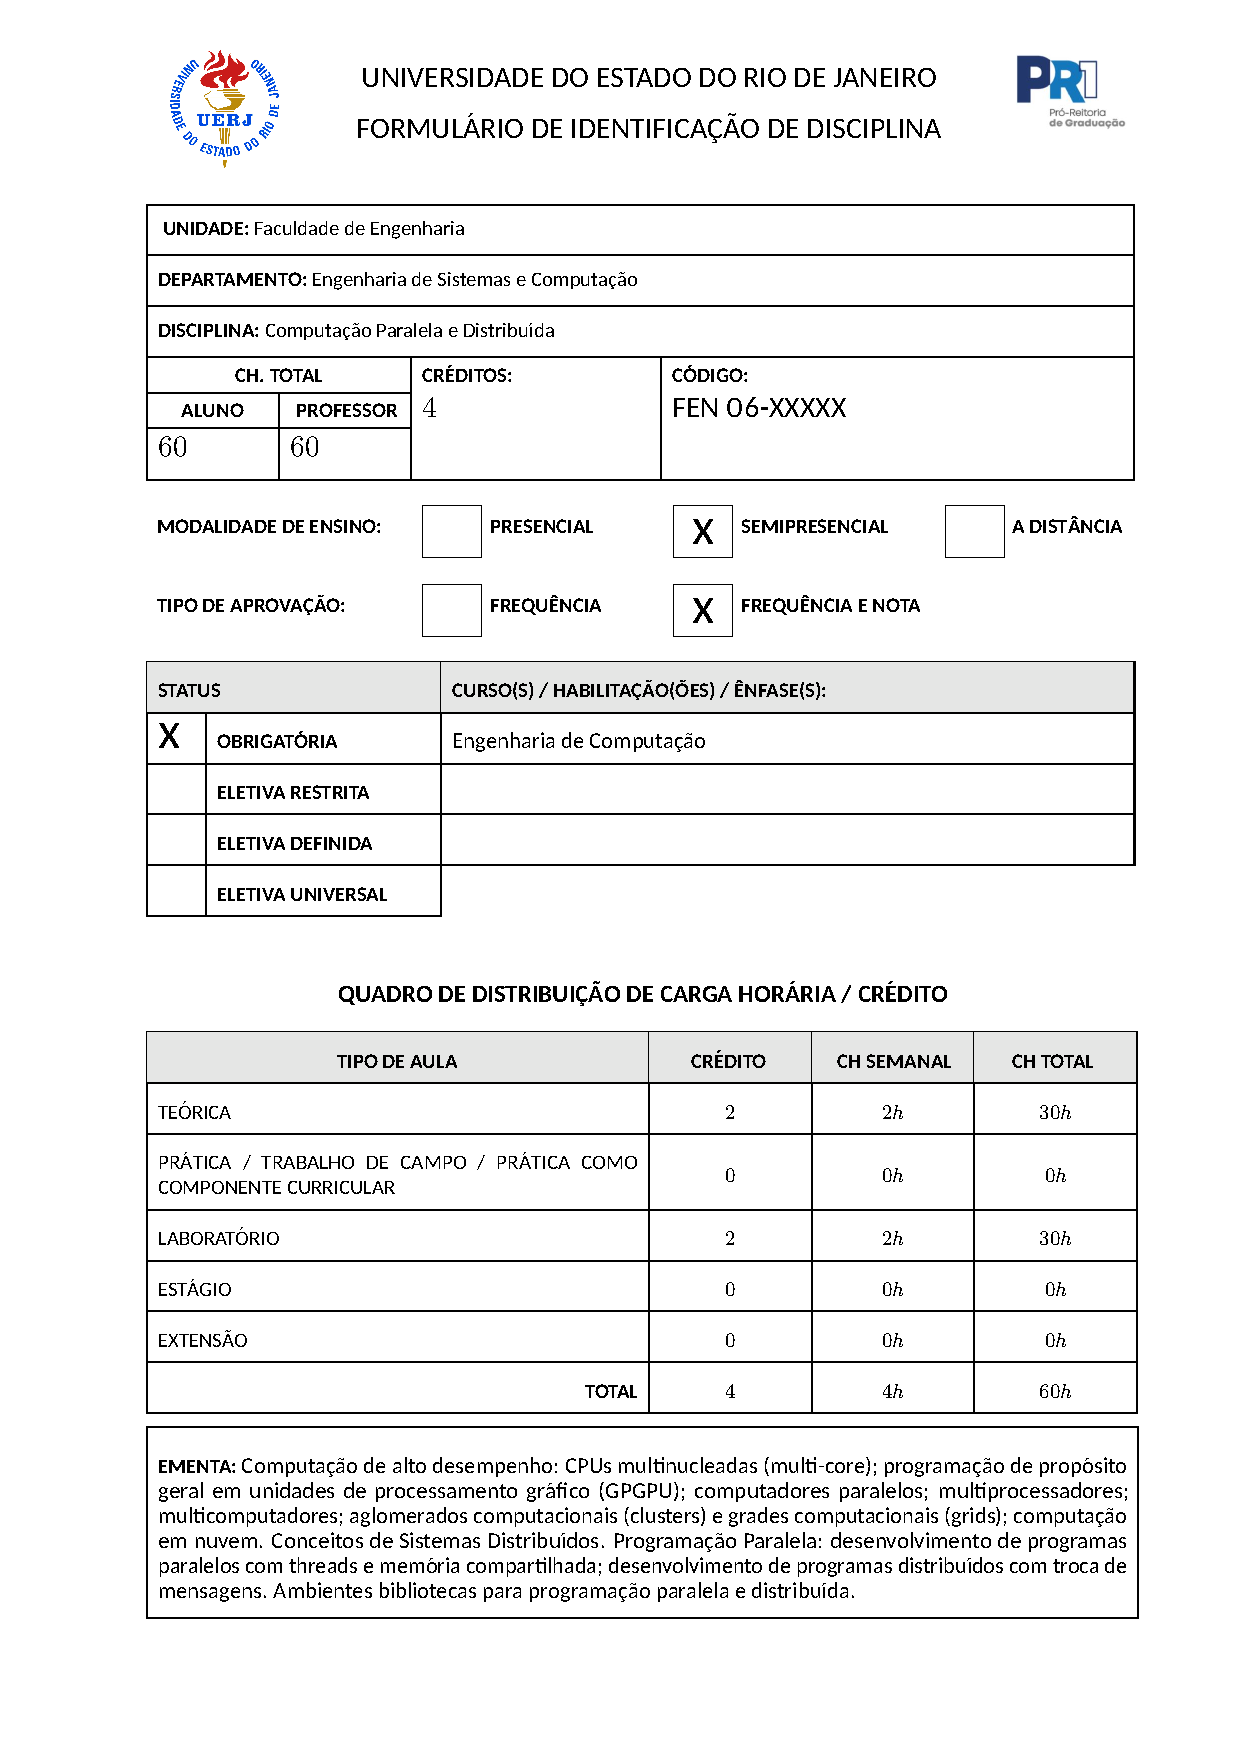
\includepdf[pages=-,addtotoc={1,section,1,{\CompParal},},pagecommand={\thispagestyle{fancy}}]{ementas/ComputacaoParalela.pdf}
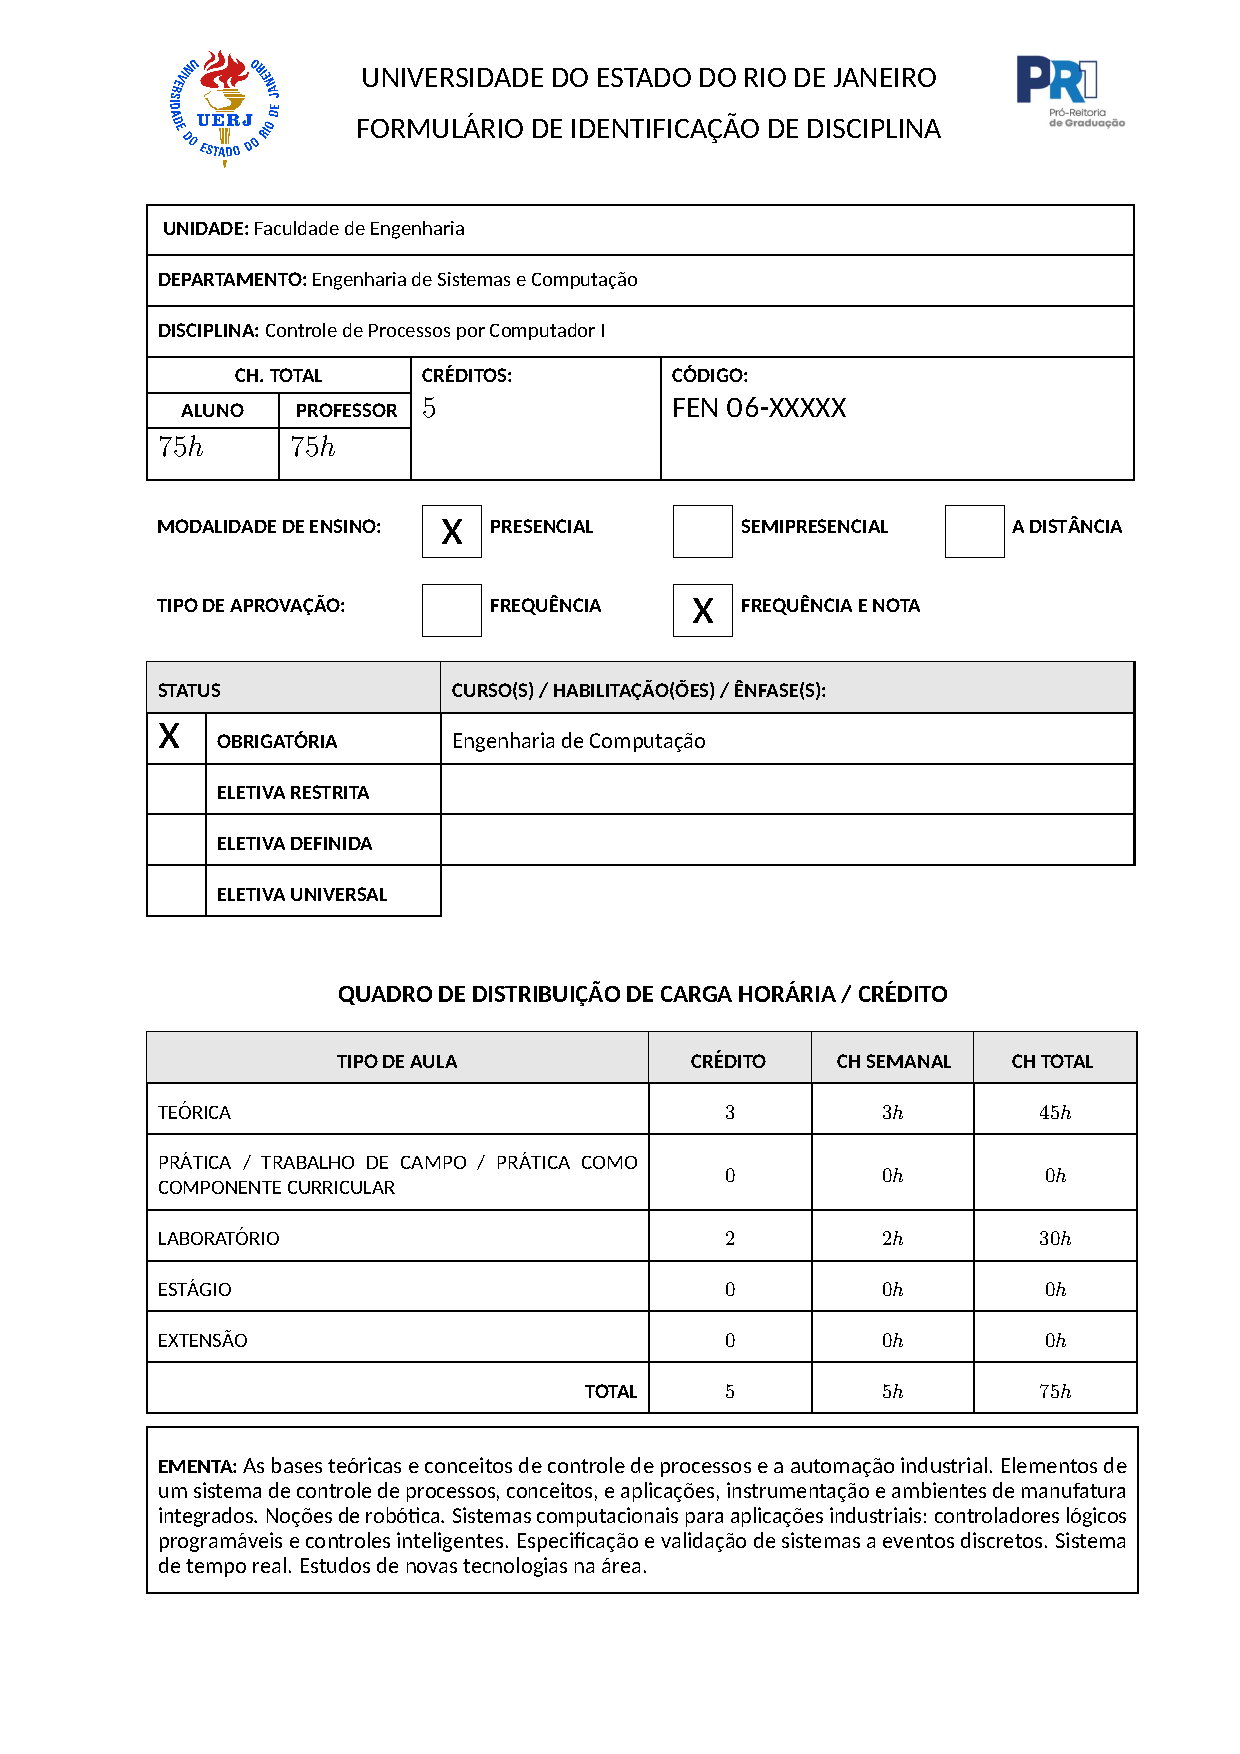
\includepdf[pages=-,addtotoc={1,section,1,{\Control},},pagecommand={\thispagestyle{fancy}}]{ementas/ControleDeProcessosPorComputador.pdf}
\includepdf[pages=-,addtotoc={1,section,1,{\FisIII},},pagecommand={\thispagestyle{fancy}}]{ementasExternas/eletromagnetismo_basico_experimental.pdf}
\includepdf[pages=-,addtotoc={1,section,1,{\FisEIII},},pagecommand={\thispagestyle{fancy}}]{ementasExternas/eletromagnetismo_basico_teorico.pdf}
\includepdf[pages=-,addtotoc={1,section,1,{\Empre},},pagecommand={\thispagestyle{fancy}}]{ementasExternas/empreendedorismo_na_engenharia.pdf}
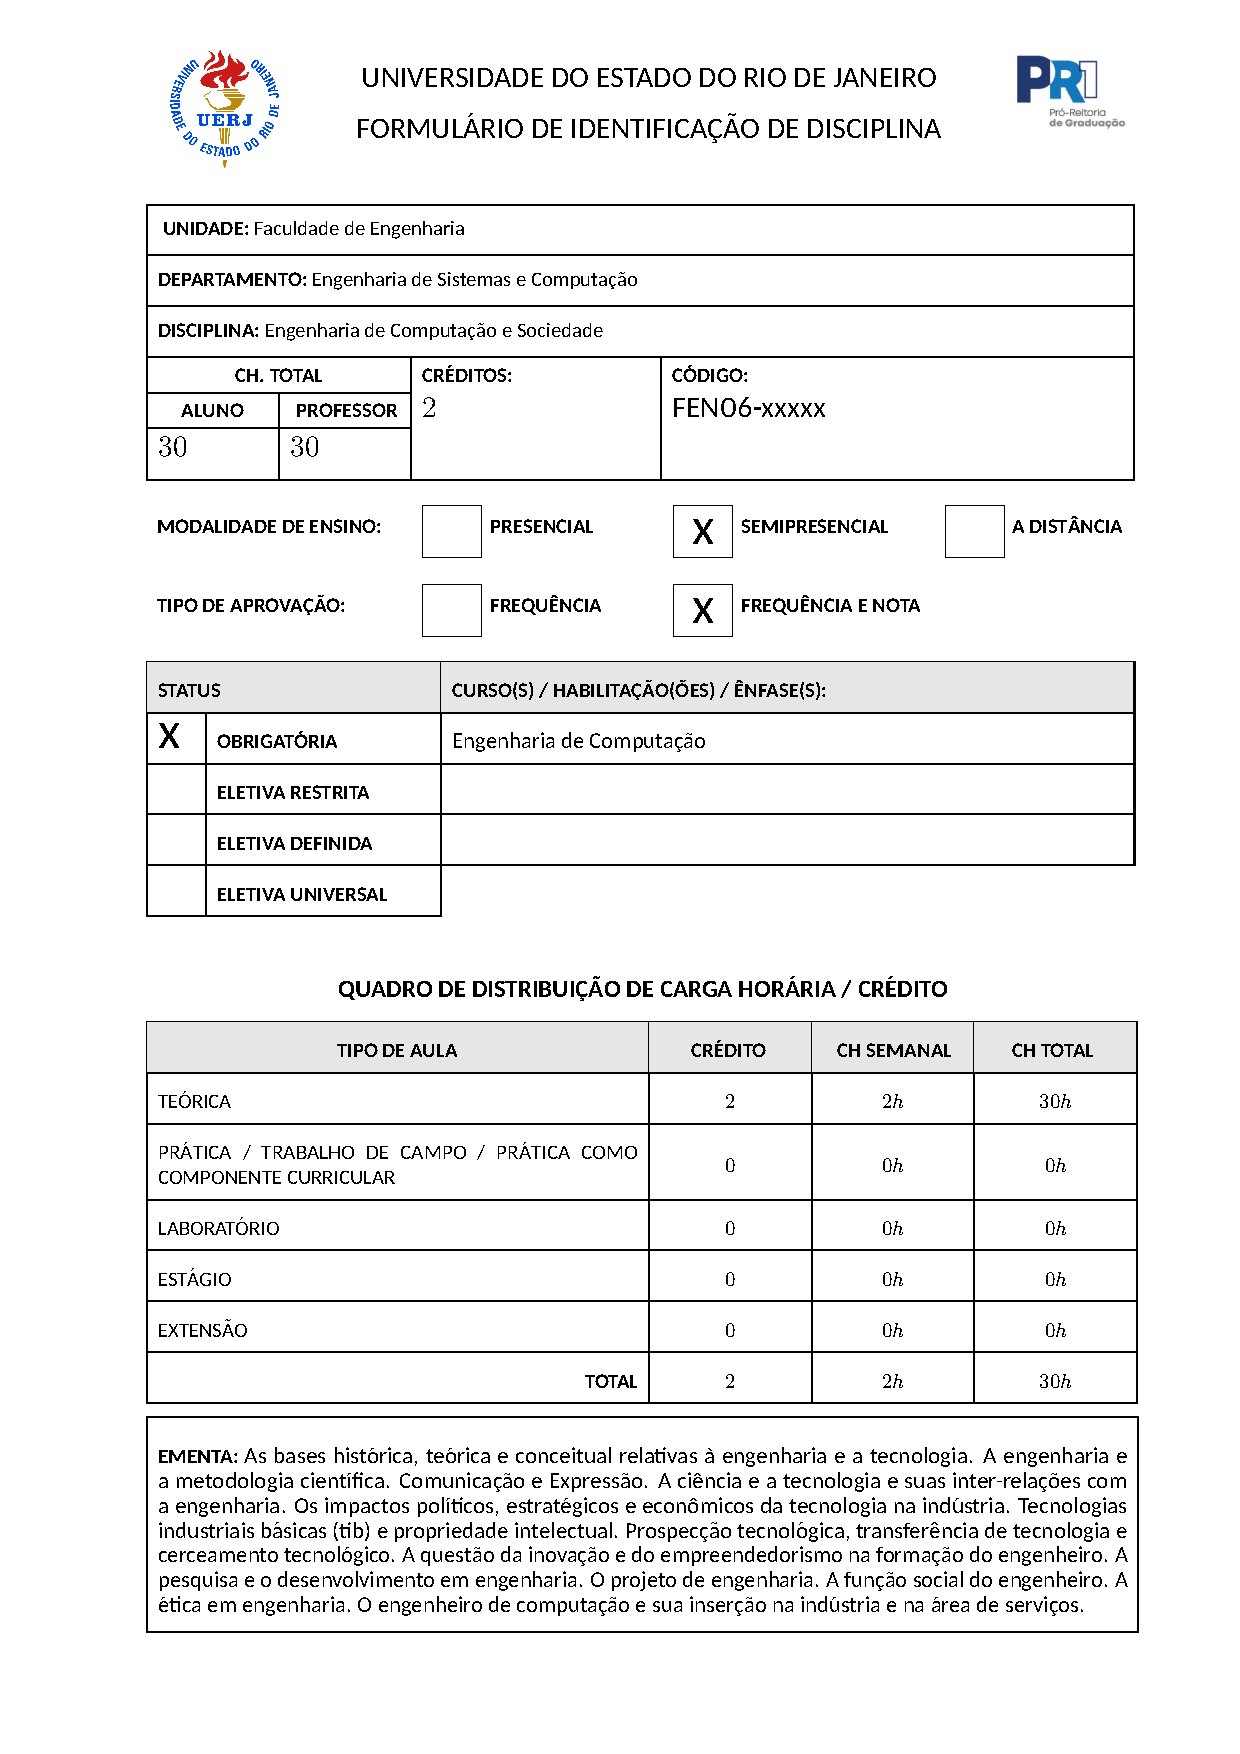
\includepdf[pages=-,addtotoc={1,section,1,{\EngCompSoc},},pagecommand={\thispagestyle{fancy}}]{ementas/EngenhariaDeComputacaoESociedade.pdf}
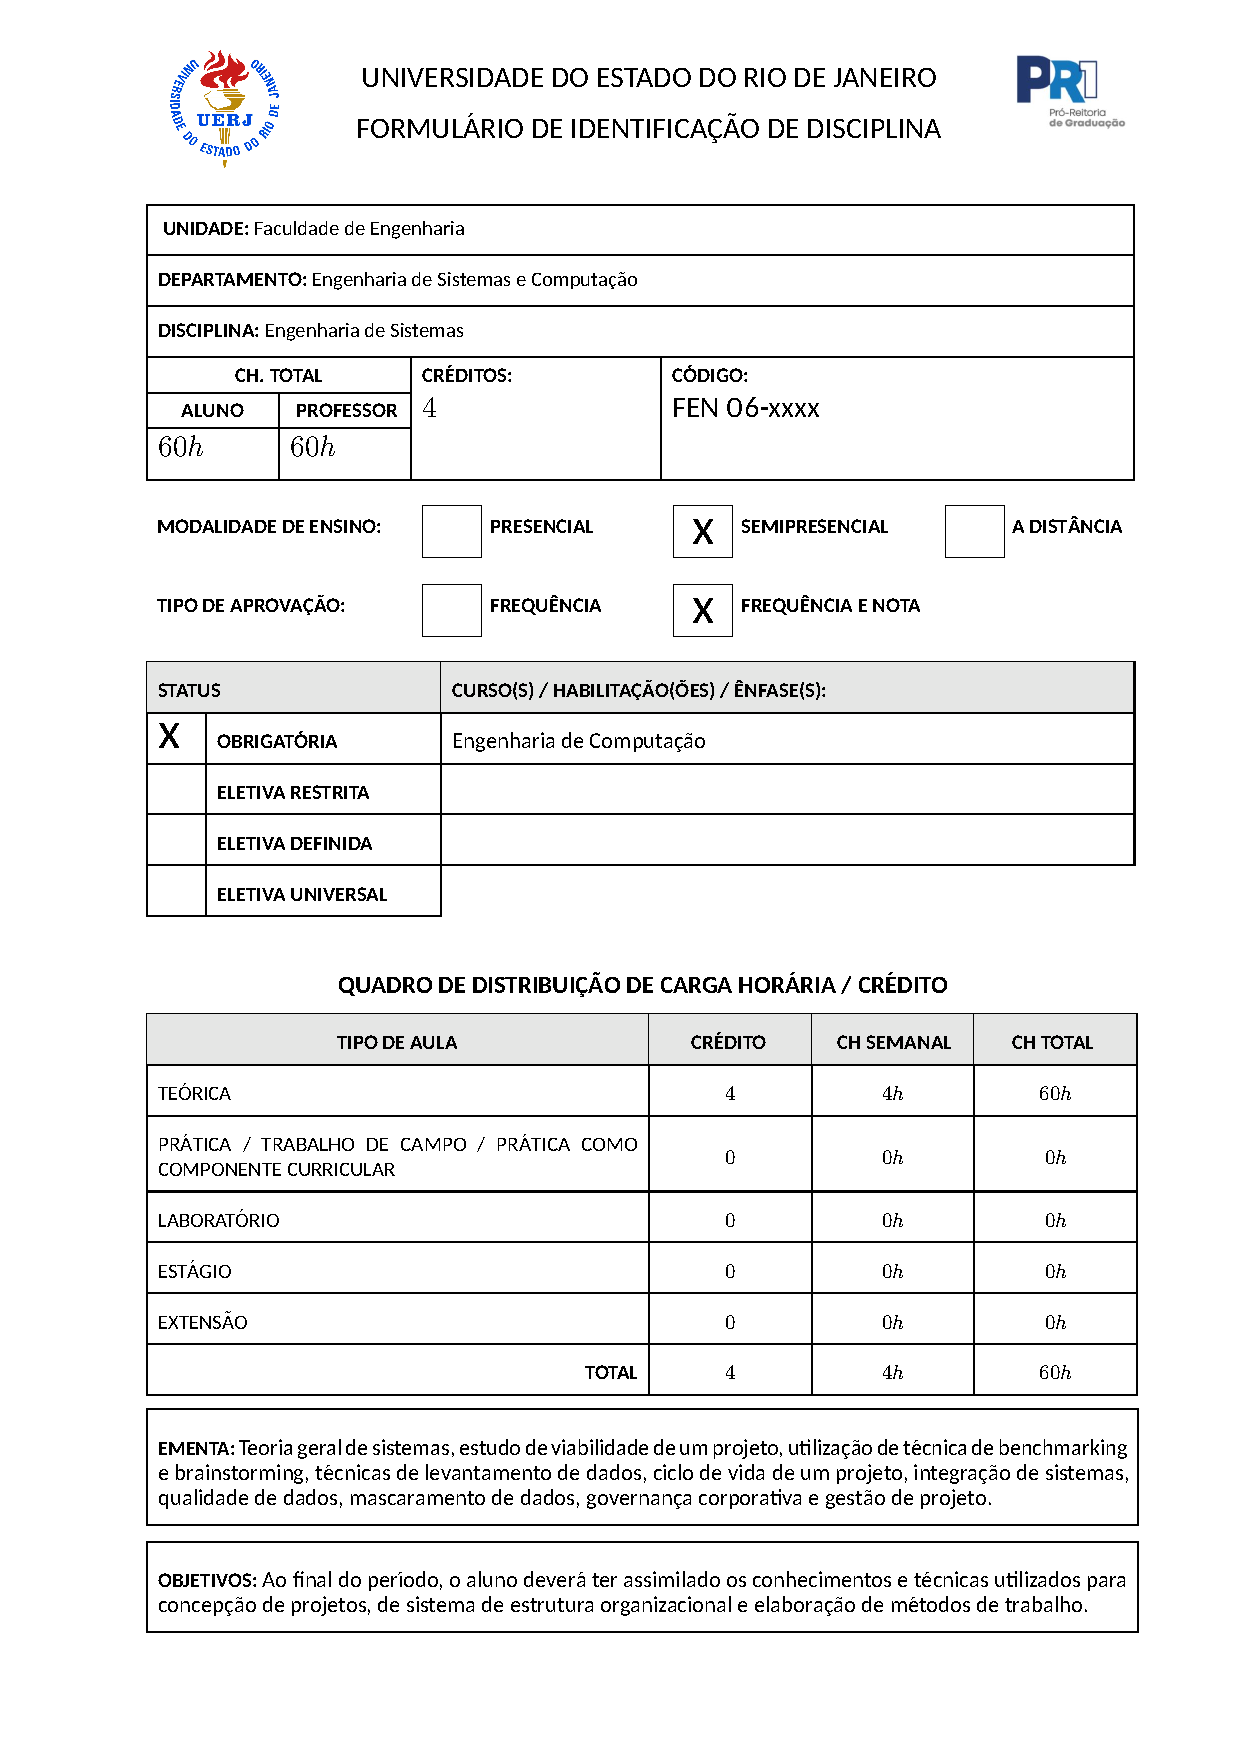
\includepdf[pages=-,addtotoc={1,section,1,{\EngSistA},},pagecommand={\thispagestyle{fancy}}]{ementas/EngenhariaDeSistemas.pdf}
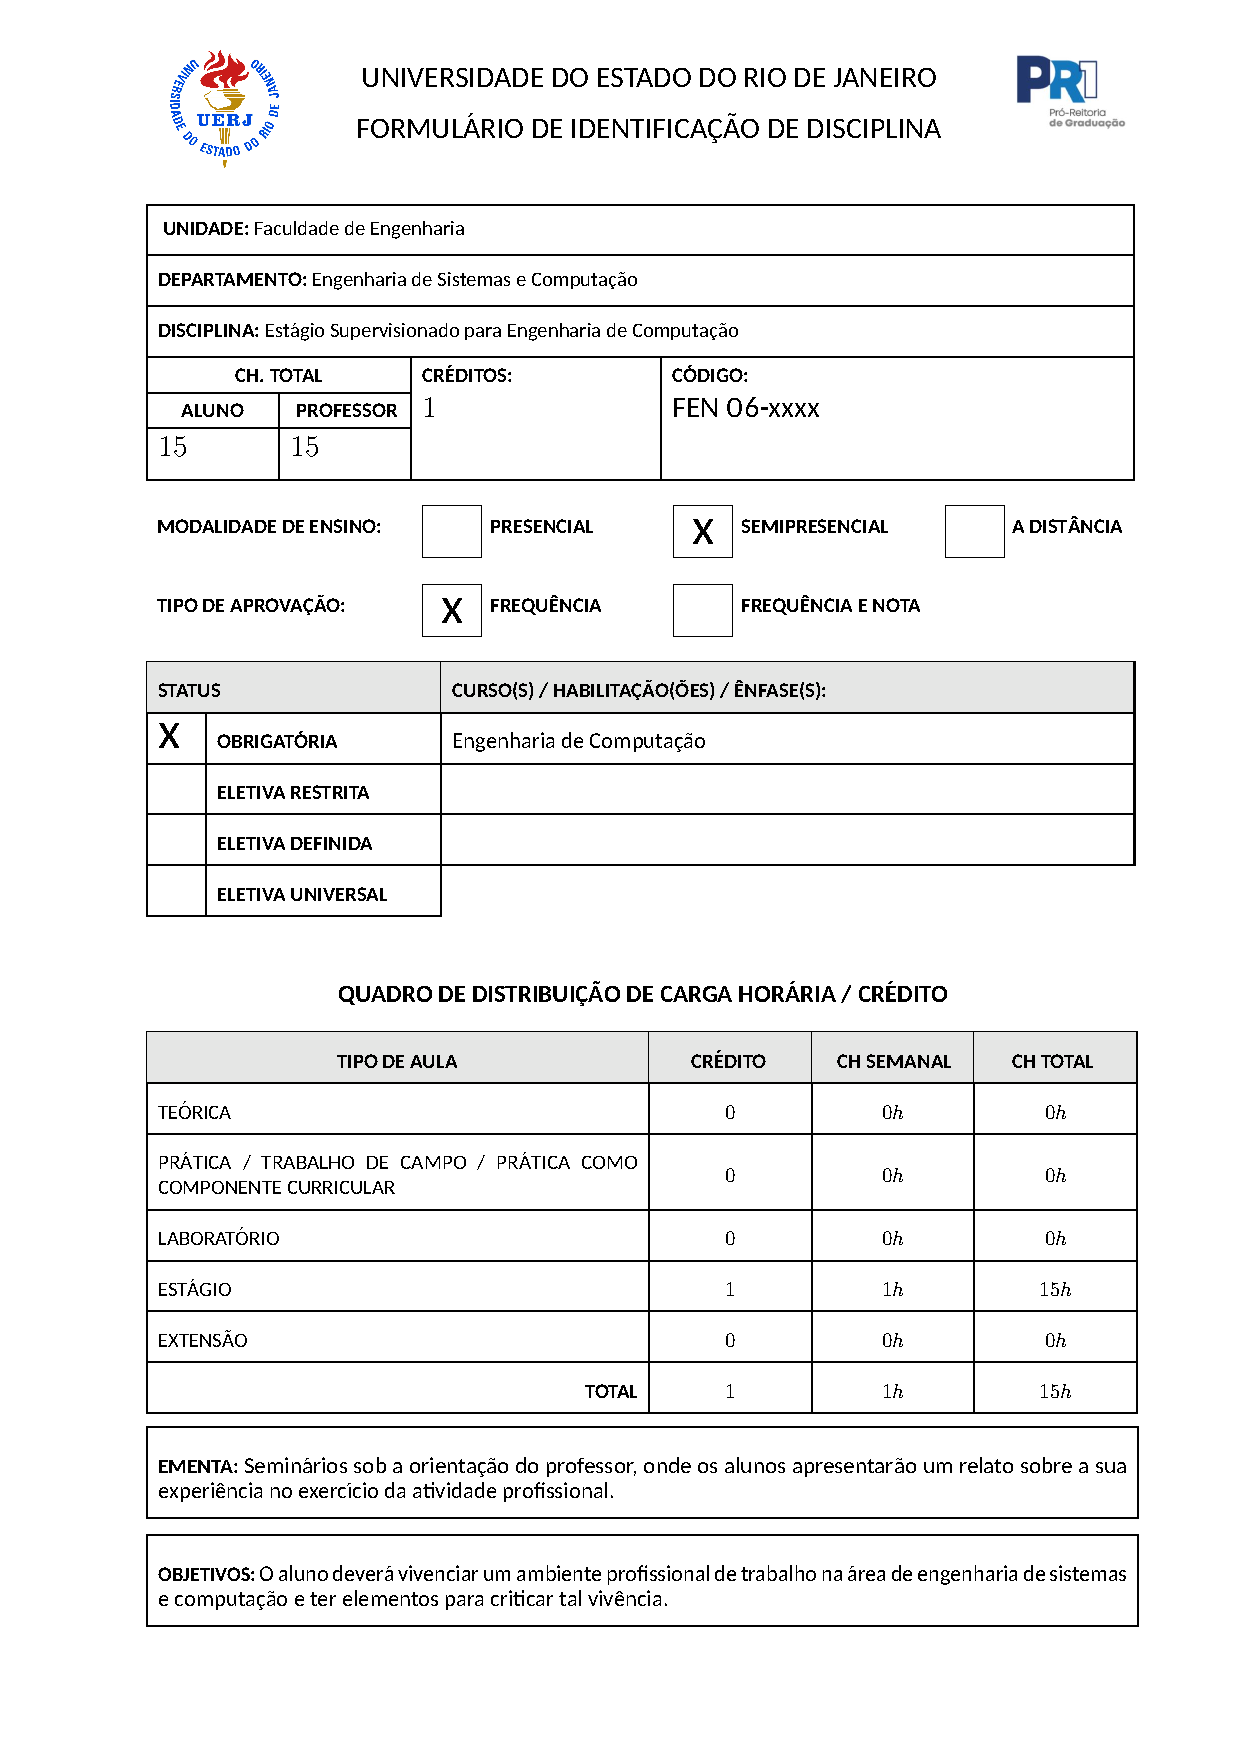
\includepdf[pages=-,addtotoc={1,section,1,{\EstSup},},pagecommand={\thispagestyle{fancy}}]{ementas/EstagioSupervisionadoXIA.pdf}
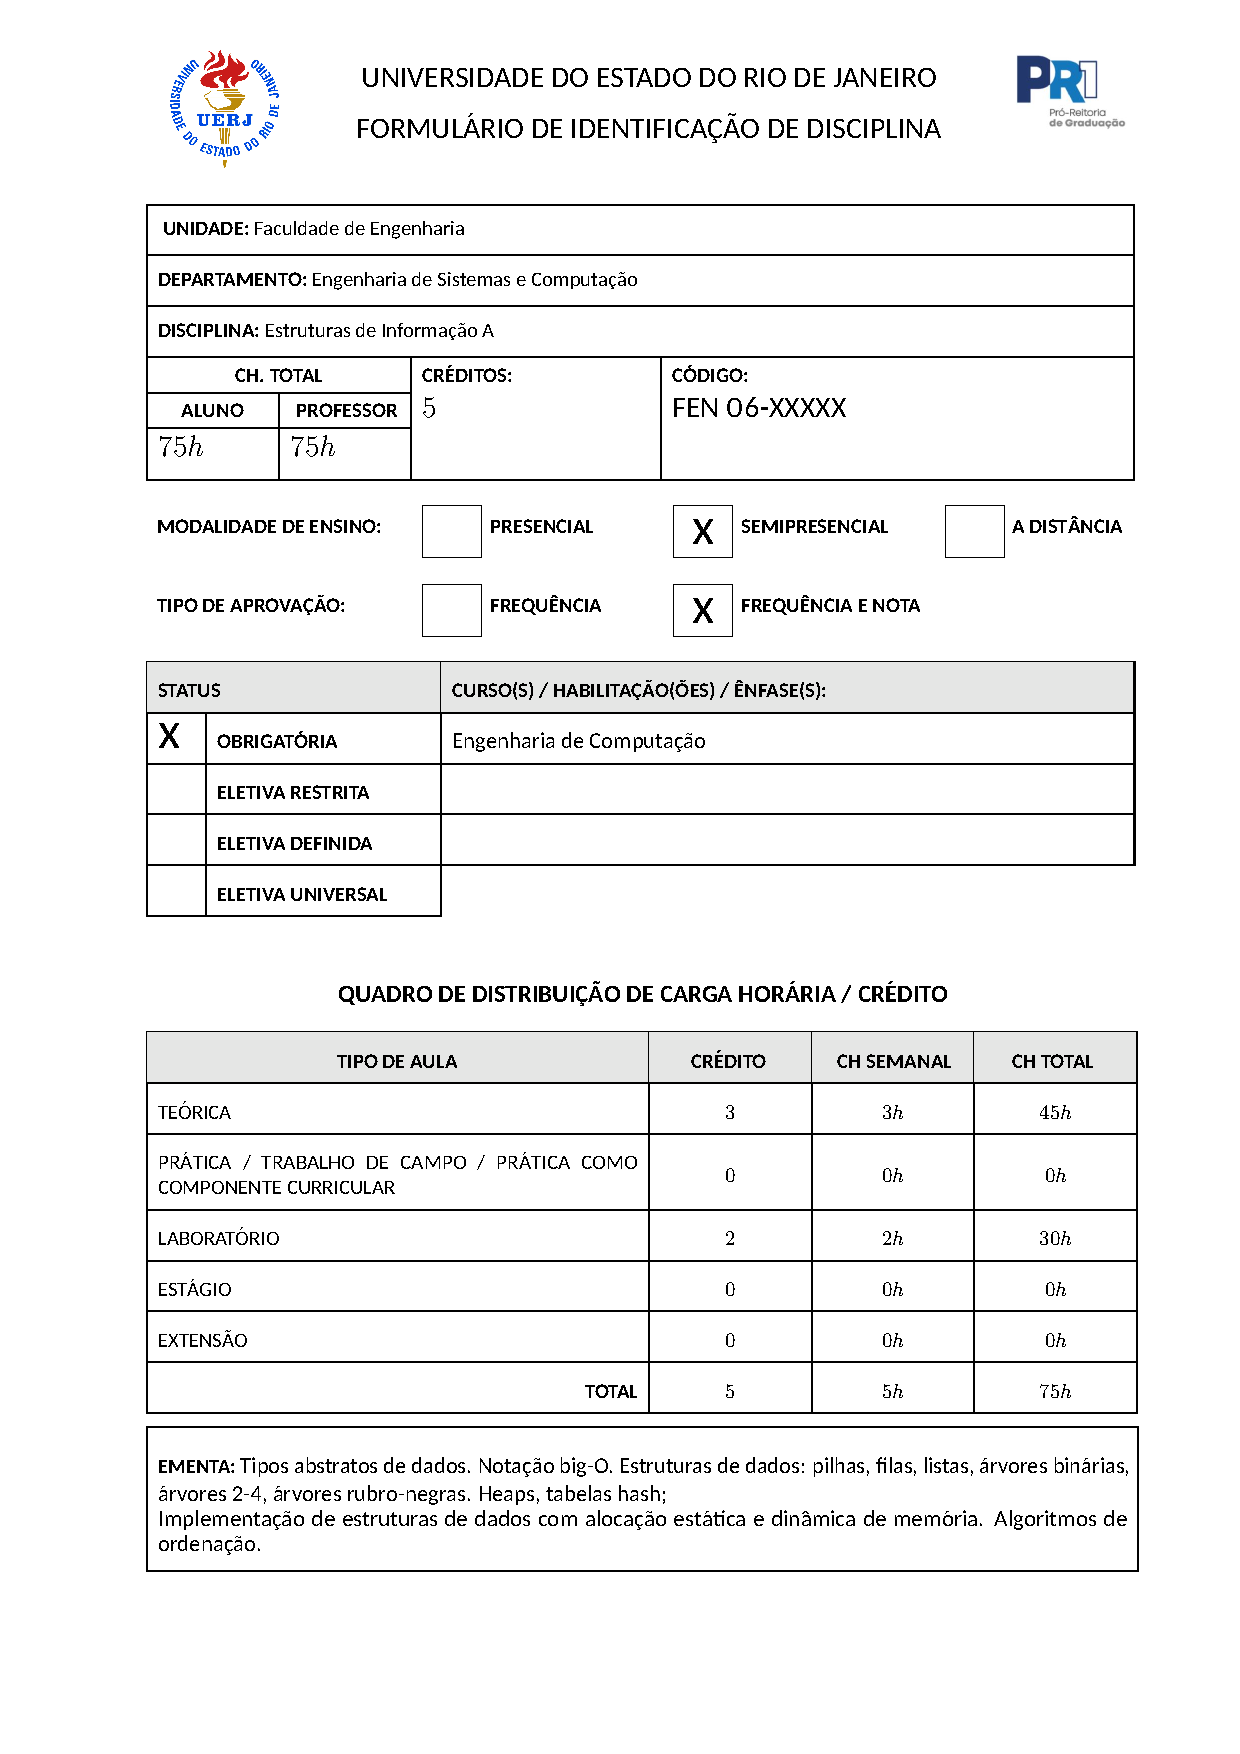
\includepdf[pages=-,addtotoc={1,section,1,{\EstrInf},},pagecommand={\thispagestyle{fancy}}]{ementas/EstruturasDeInformacao.pdf}
\includepdf[pages=-,addtotoc={1,section,1,{\FisEI},},pagecommand={\thispagestyle{fancy}}]{ementasExternas/fisica_experimental_i.pdf}
\includepdf[pages=-,addtotoc={1,section,1,{\FisEII},},pagecommand={\thispagestyle{fancy}}]{ementasExternas/fisica_experimental_ii.pdf}
\includepdf[pages=-,addtotoc={1,section,1,{\FisEIV},},pagecommand={\thispagestyle{fancy}}]{ementasExternas/fisica_experimental_iv.pdf}
\includepdf[pages=-,addtotoc={1,section,1,{\FisI},},pagecommand={\thispagestyle{fancy}}]{ementasExternas/fisica_teorica_i.pdf}
\includepdf[pages=-,addtotoc={1,section,1,{\FisII},},pagecommand={\thispagestyle{fancy}}]{ementasExternas/fisica_teorica_ii.pdf}
\includepdf[pages=-,addtotoc={1,section,1,{\FisIV},},pagecommand={\thispagestyle{fancy}}]{ementasExternas/fisica_teorica_iv.pdf}
% Eletromagnetismo Básico Teórico era 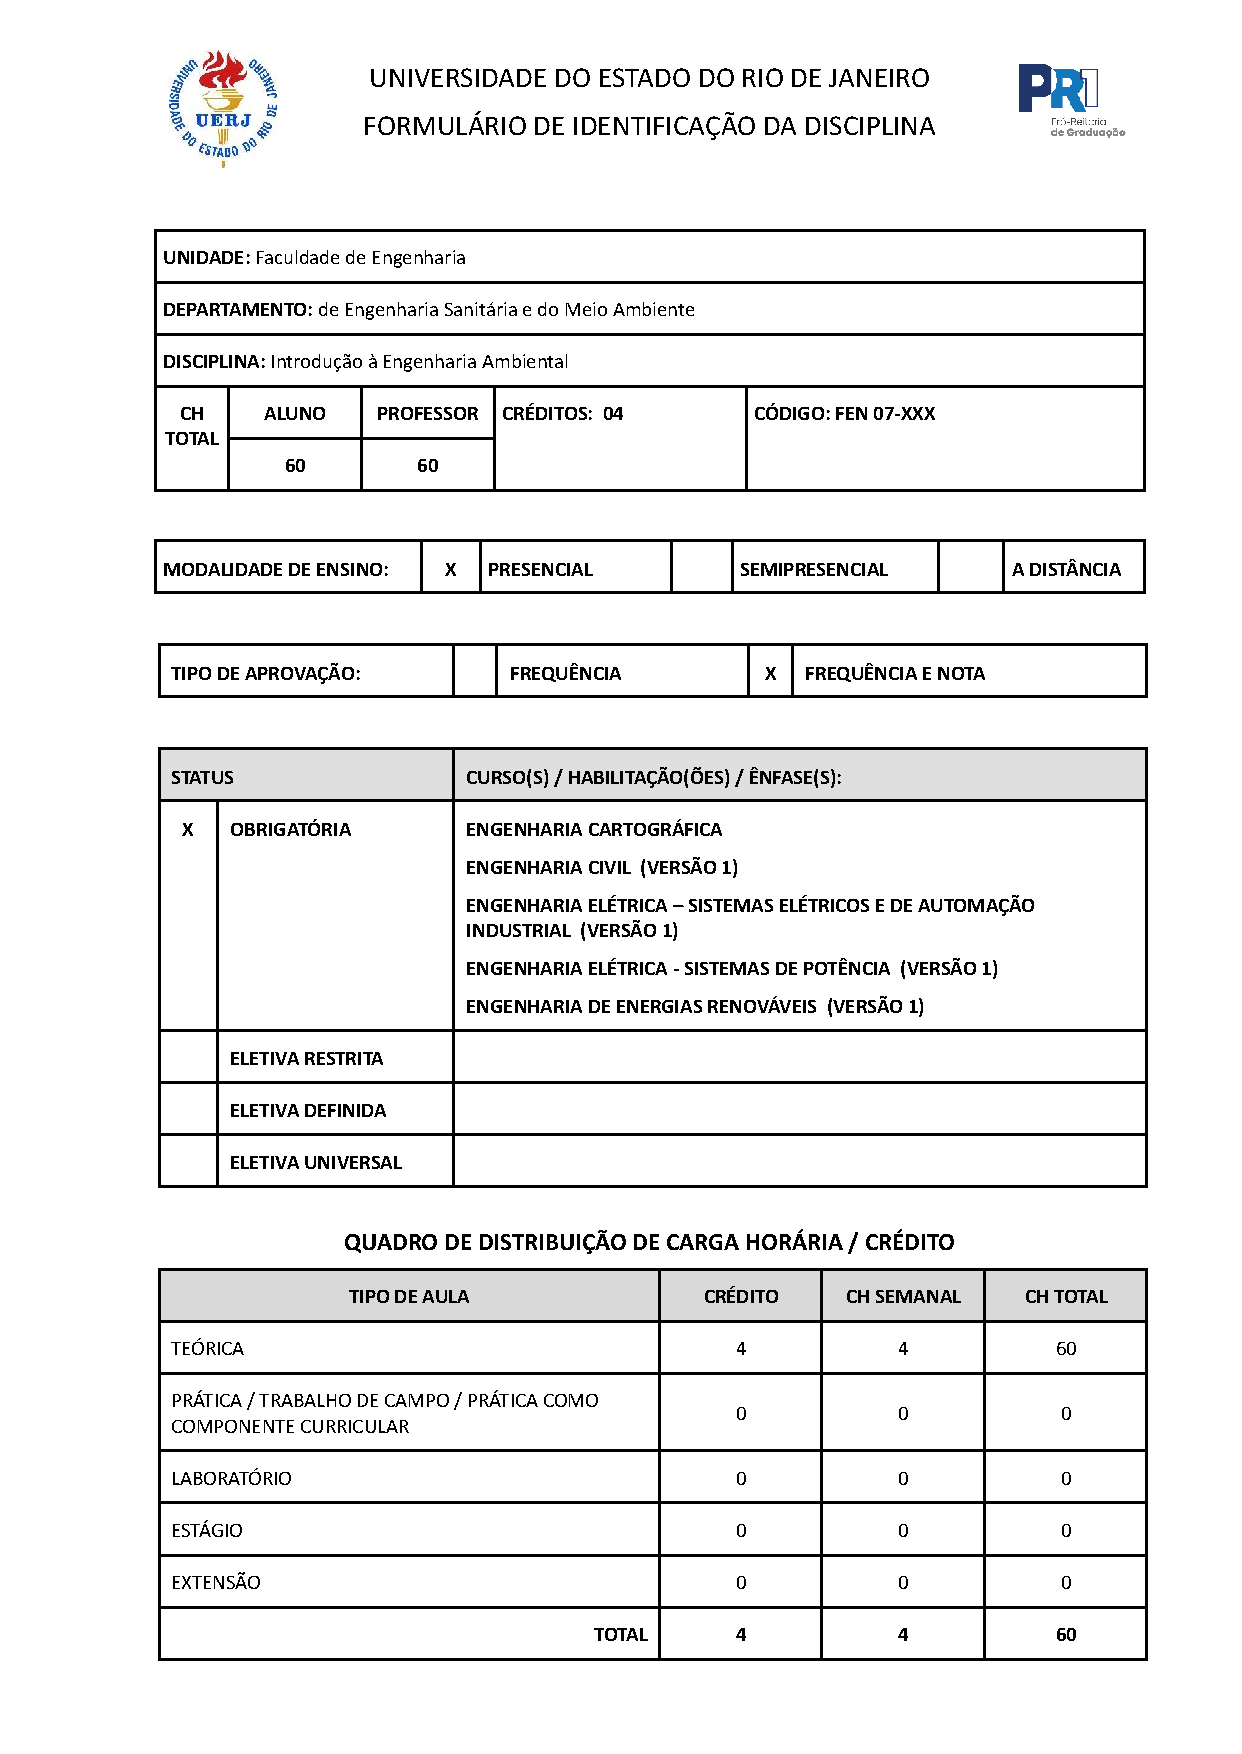
\includepdf[pages=-,addtotoc={1,section,1,{\IntAmb},},pagecommand={\thispagestyle{fancy}}]{ementasExternas/Introducao_a_Engenharia_Ambiental.pdf}
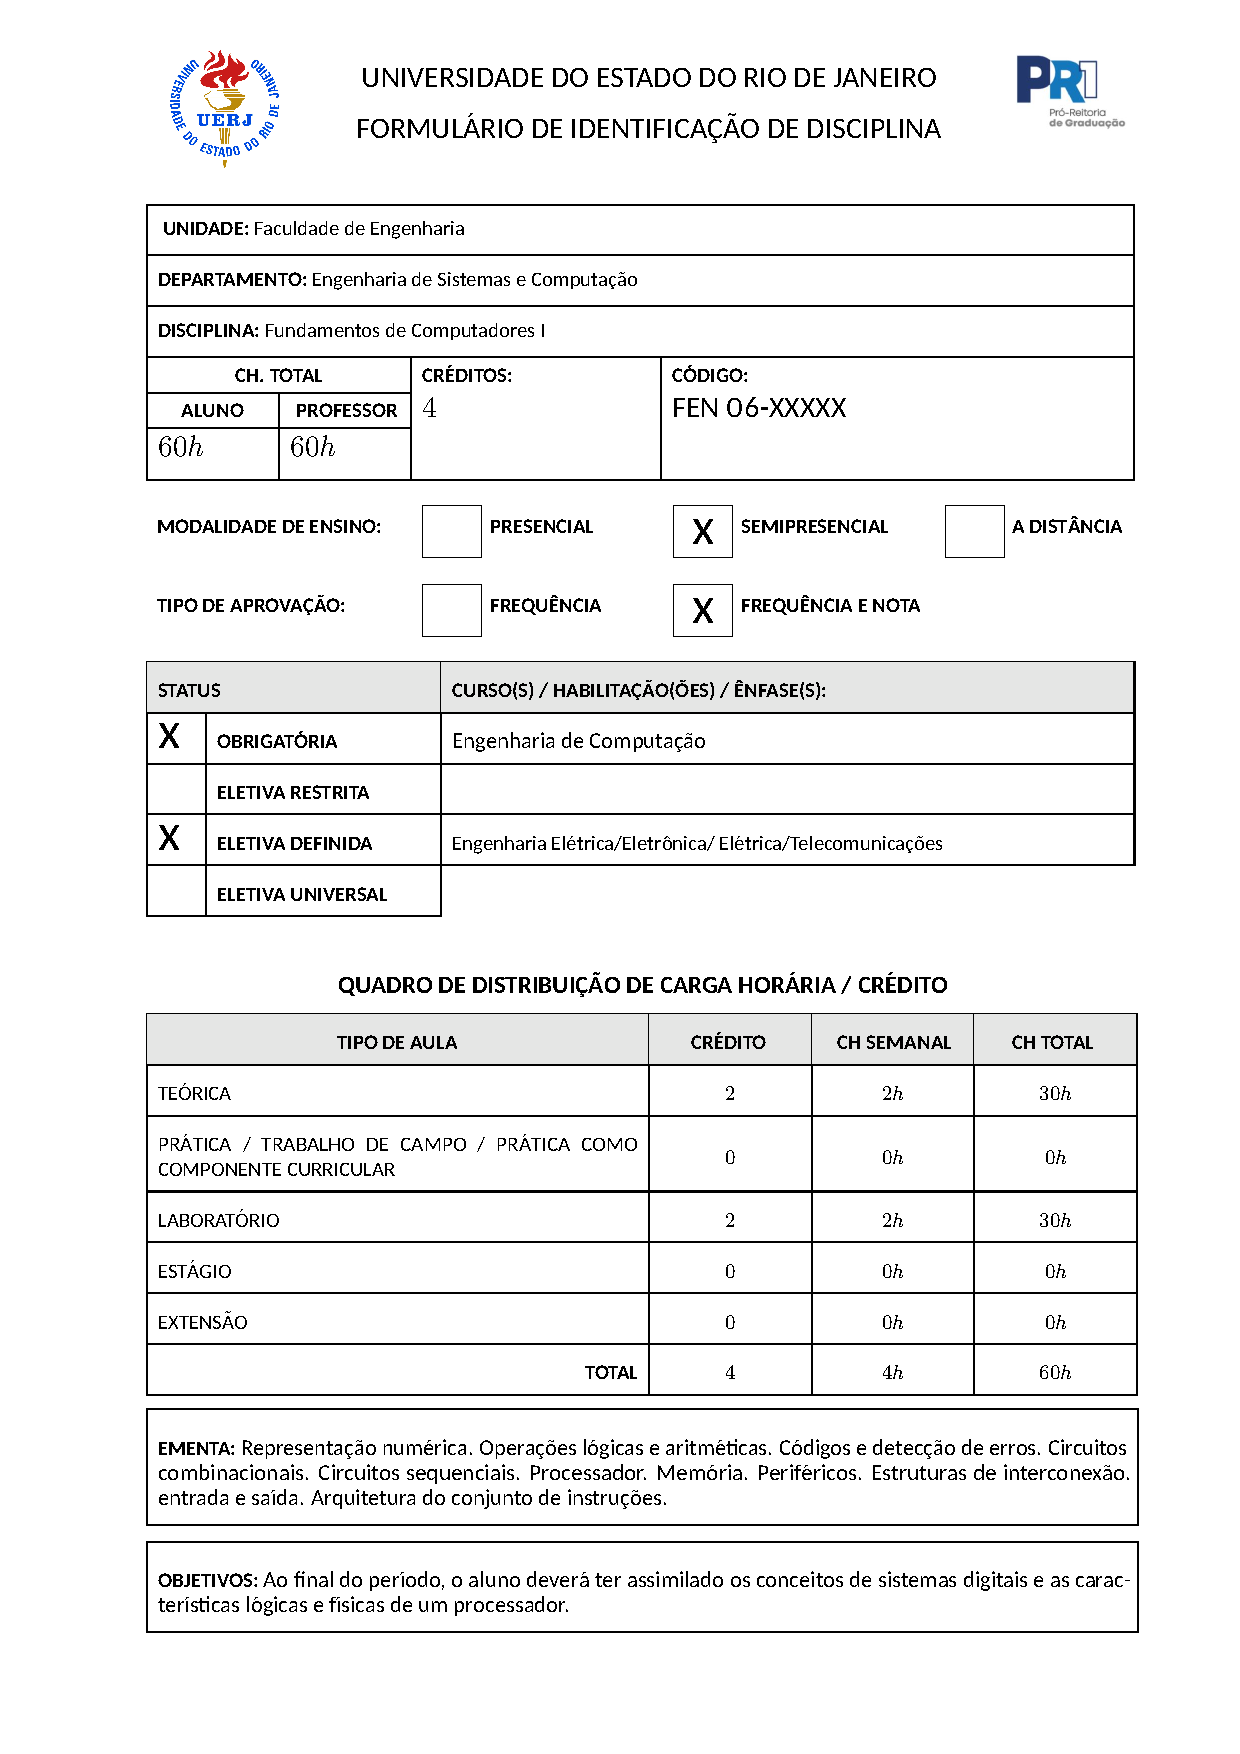
\includepdf[pages=-,addtotoc={1,section,1,{\FundComp},},pagecommand={\thispagestyle{fancy}}]{ementas/FundamentosDeComputadores.pdf}
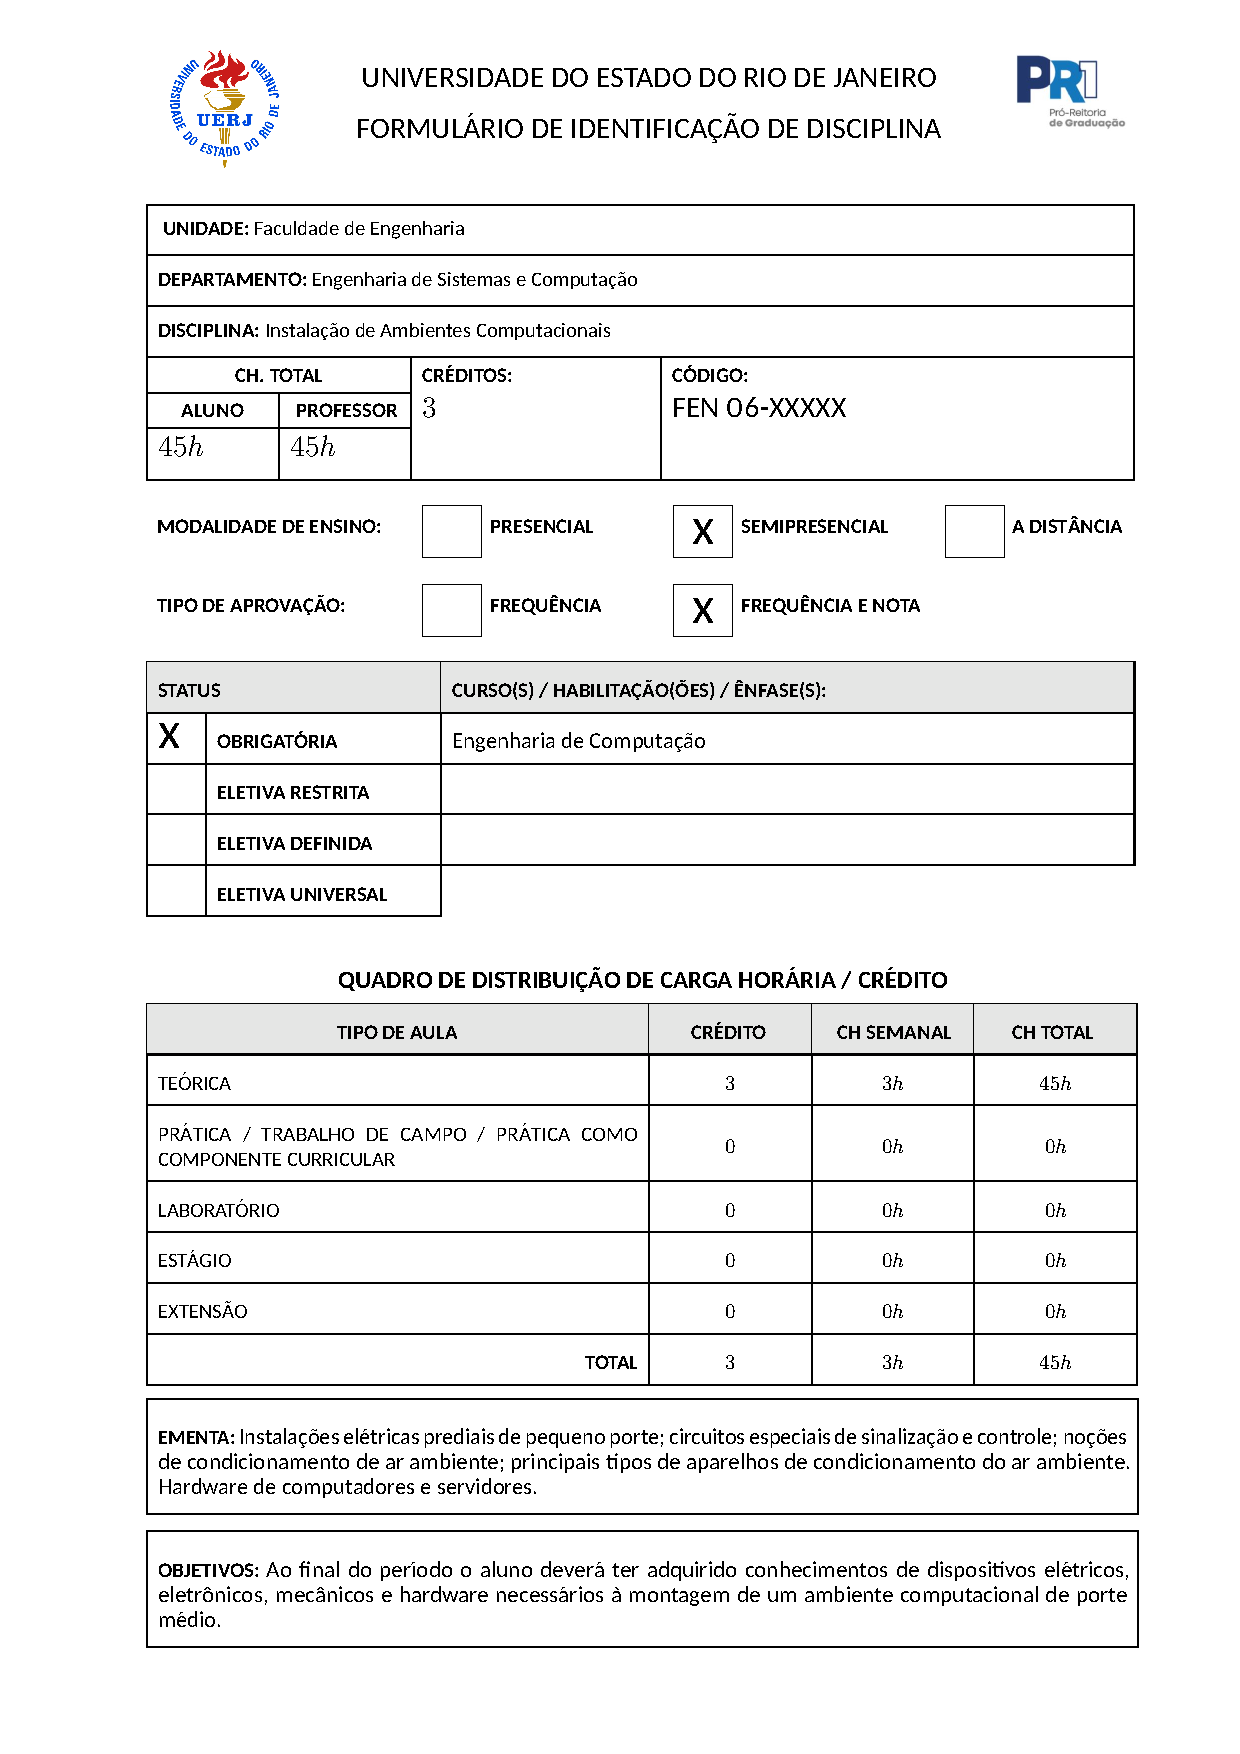
\includepdf[pages=-,addtotoc={1,section,1,{\Instala},},pagecommand={\thispagestyle{fancy}}]{ementas/instalacao_de_ambientes_computacionais.pdf}
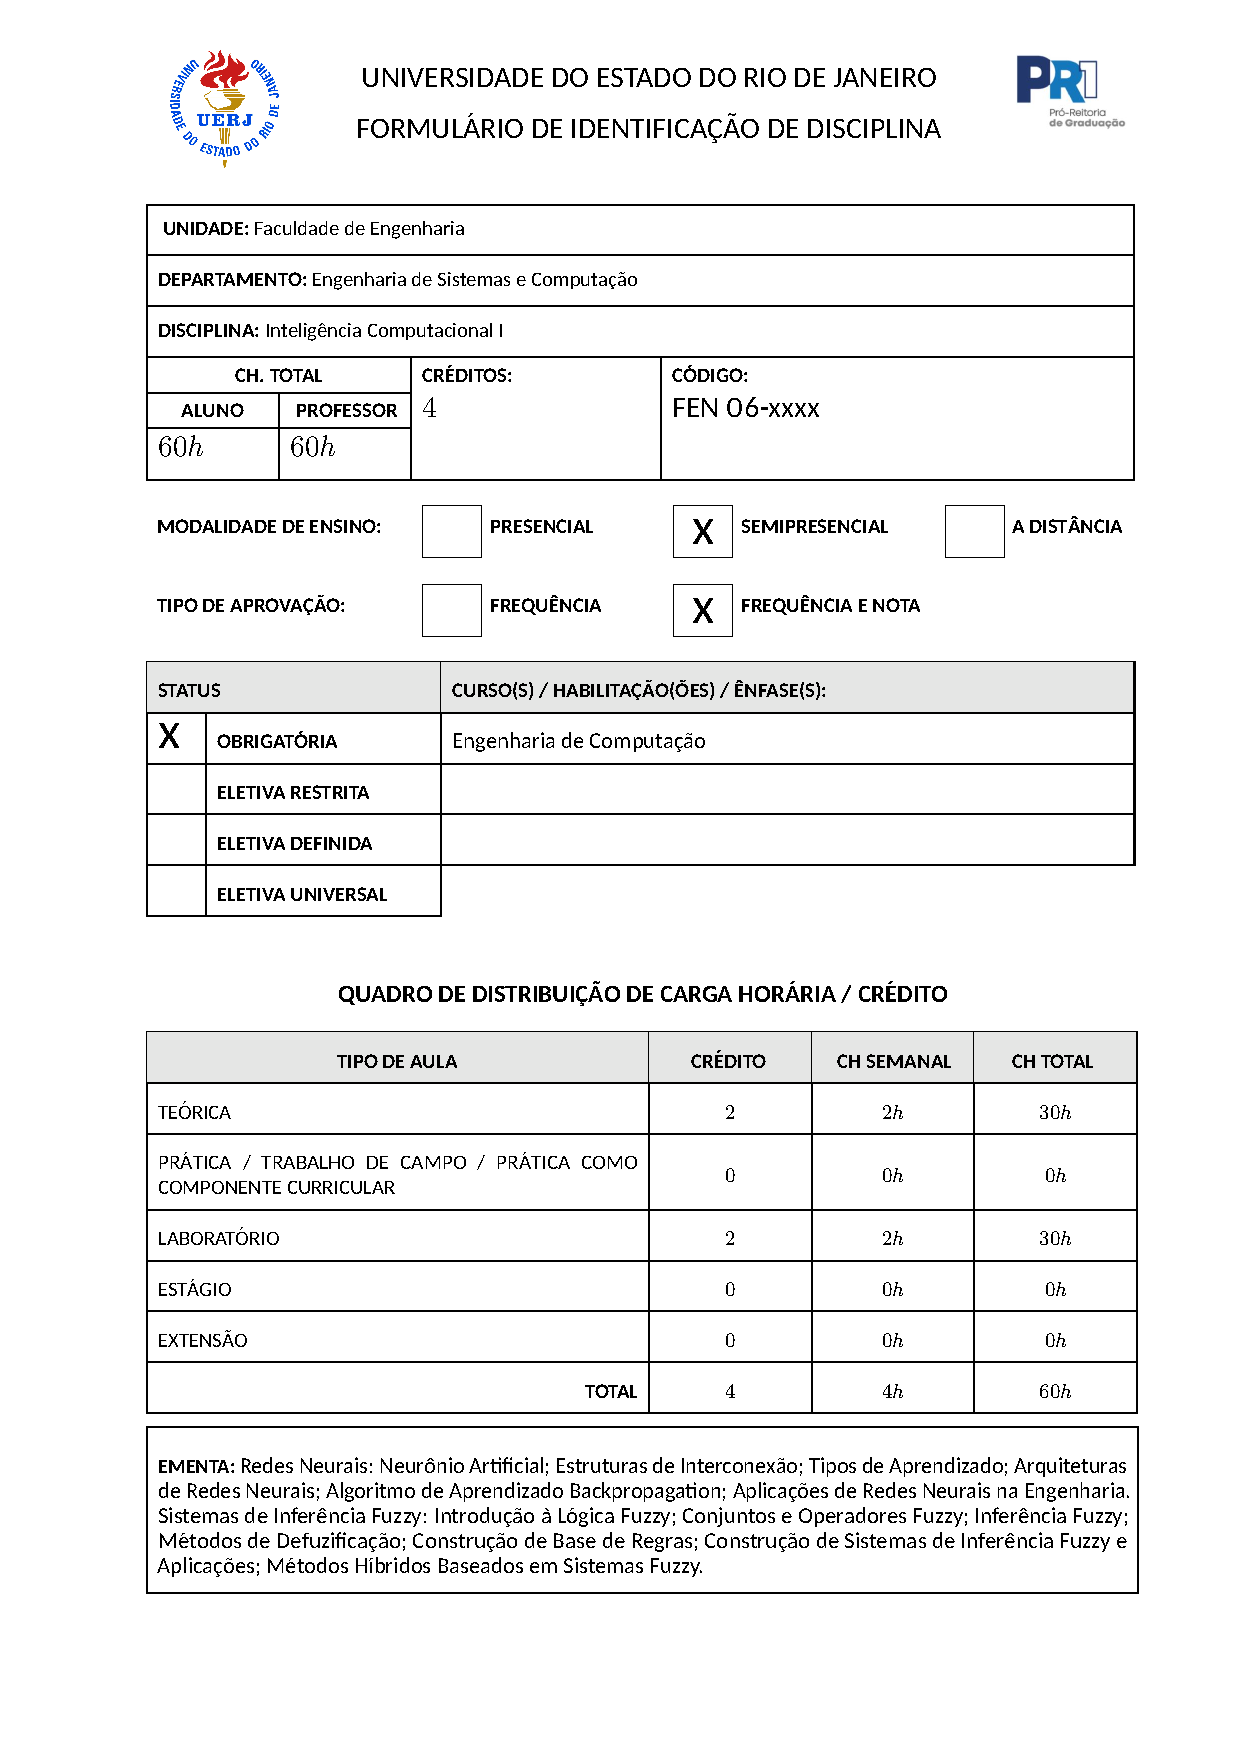
\includepdf[pages=-,addtotoc={1,section,1,{\IC},},pagecommand={\thispagestyle{fancy}}]{ementas/InteligenciaComputacional1.pdf}
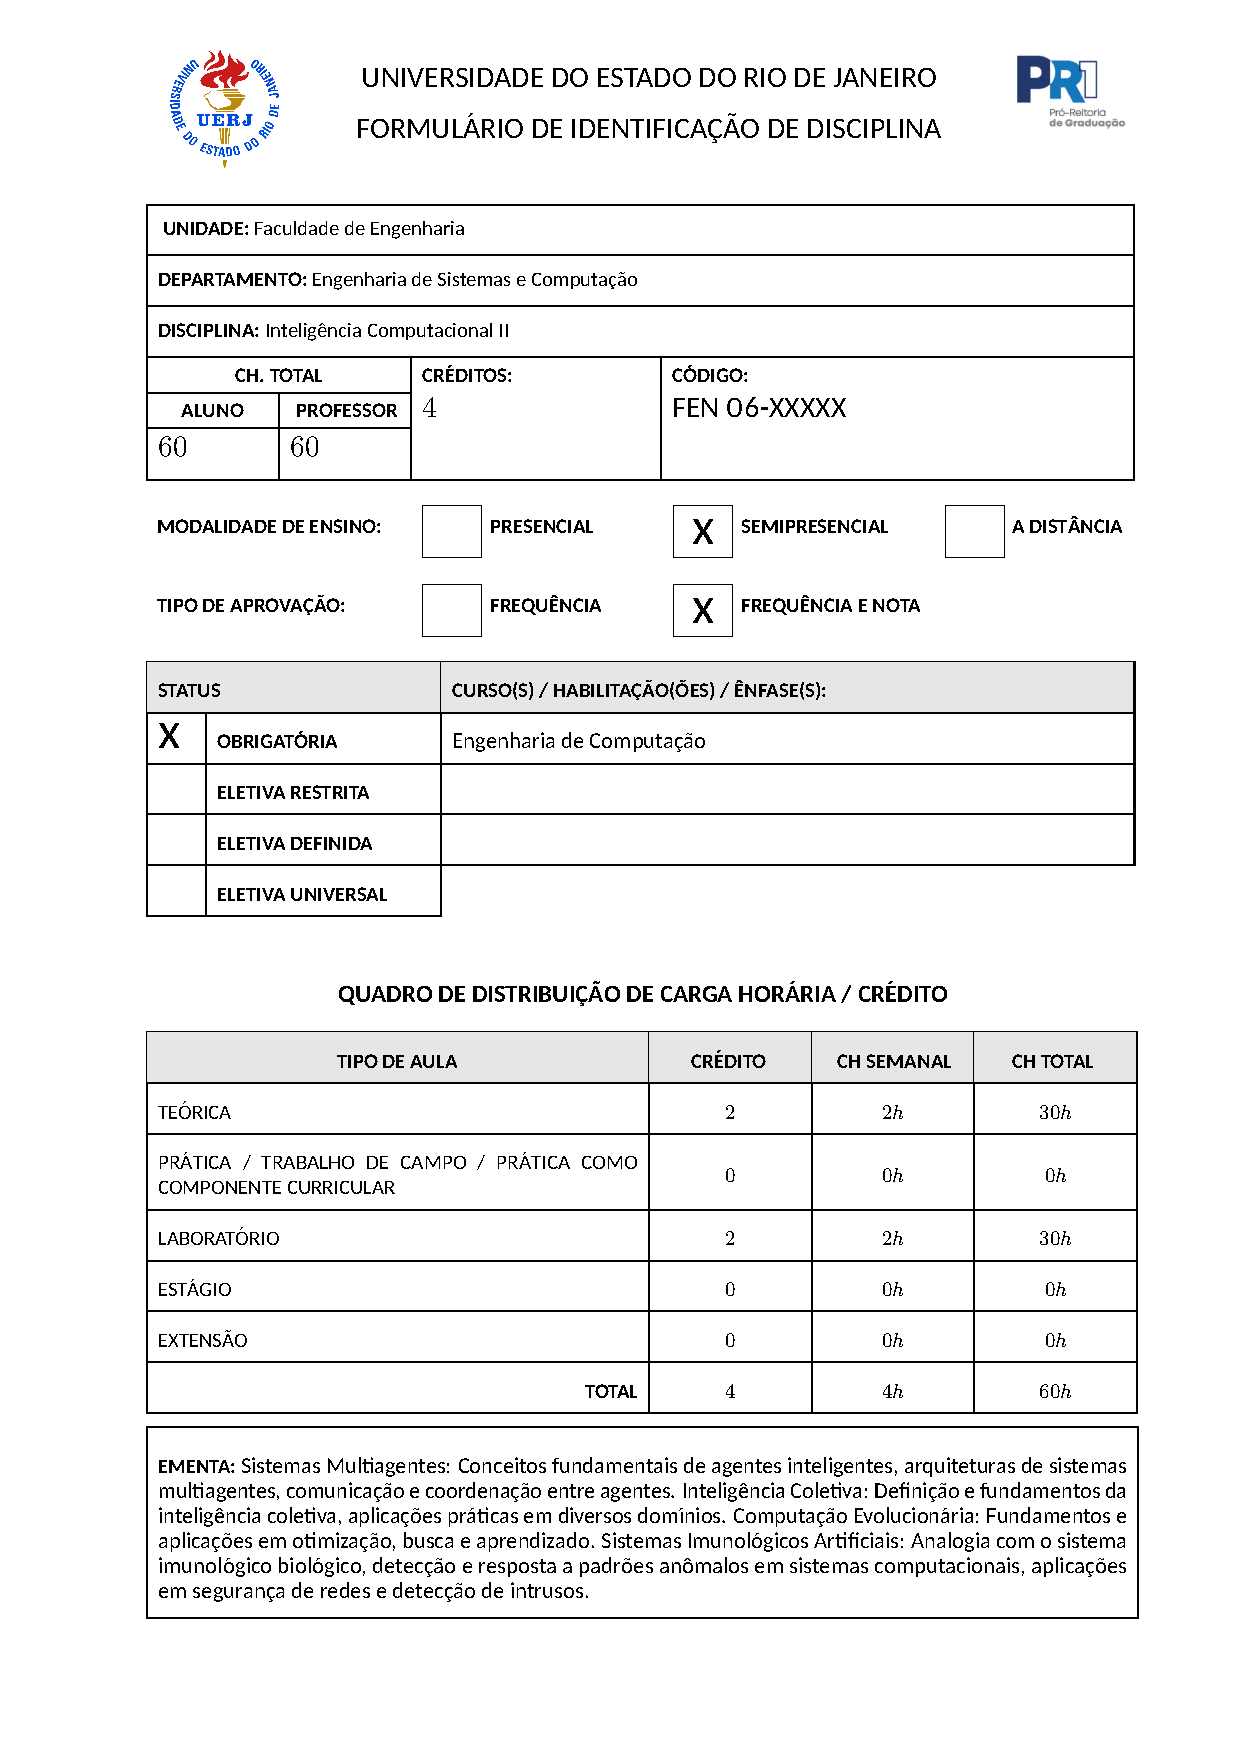
\includepdf[pages=-,addtotoc={1,section,1,{\ICII},},pagecommand={\thispagestyle{fancy}}]{ementas/InteligenciaComputacional2.pdf}
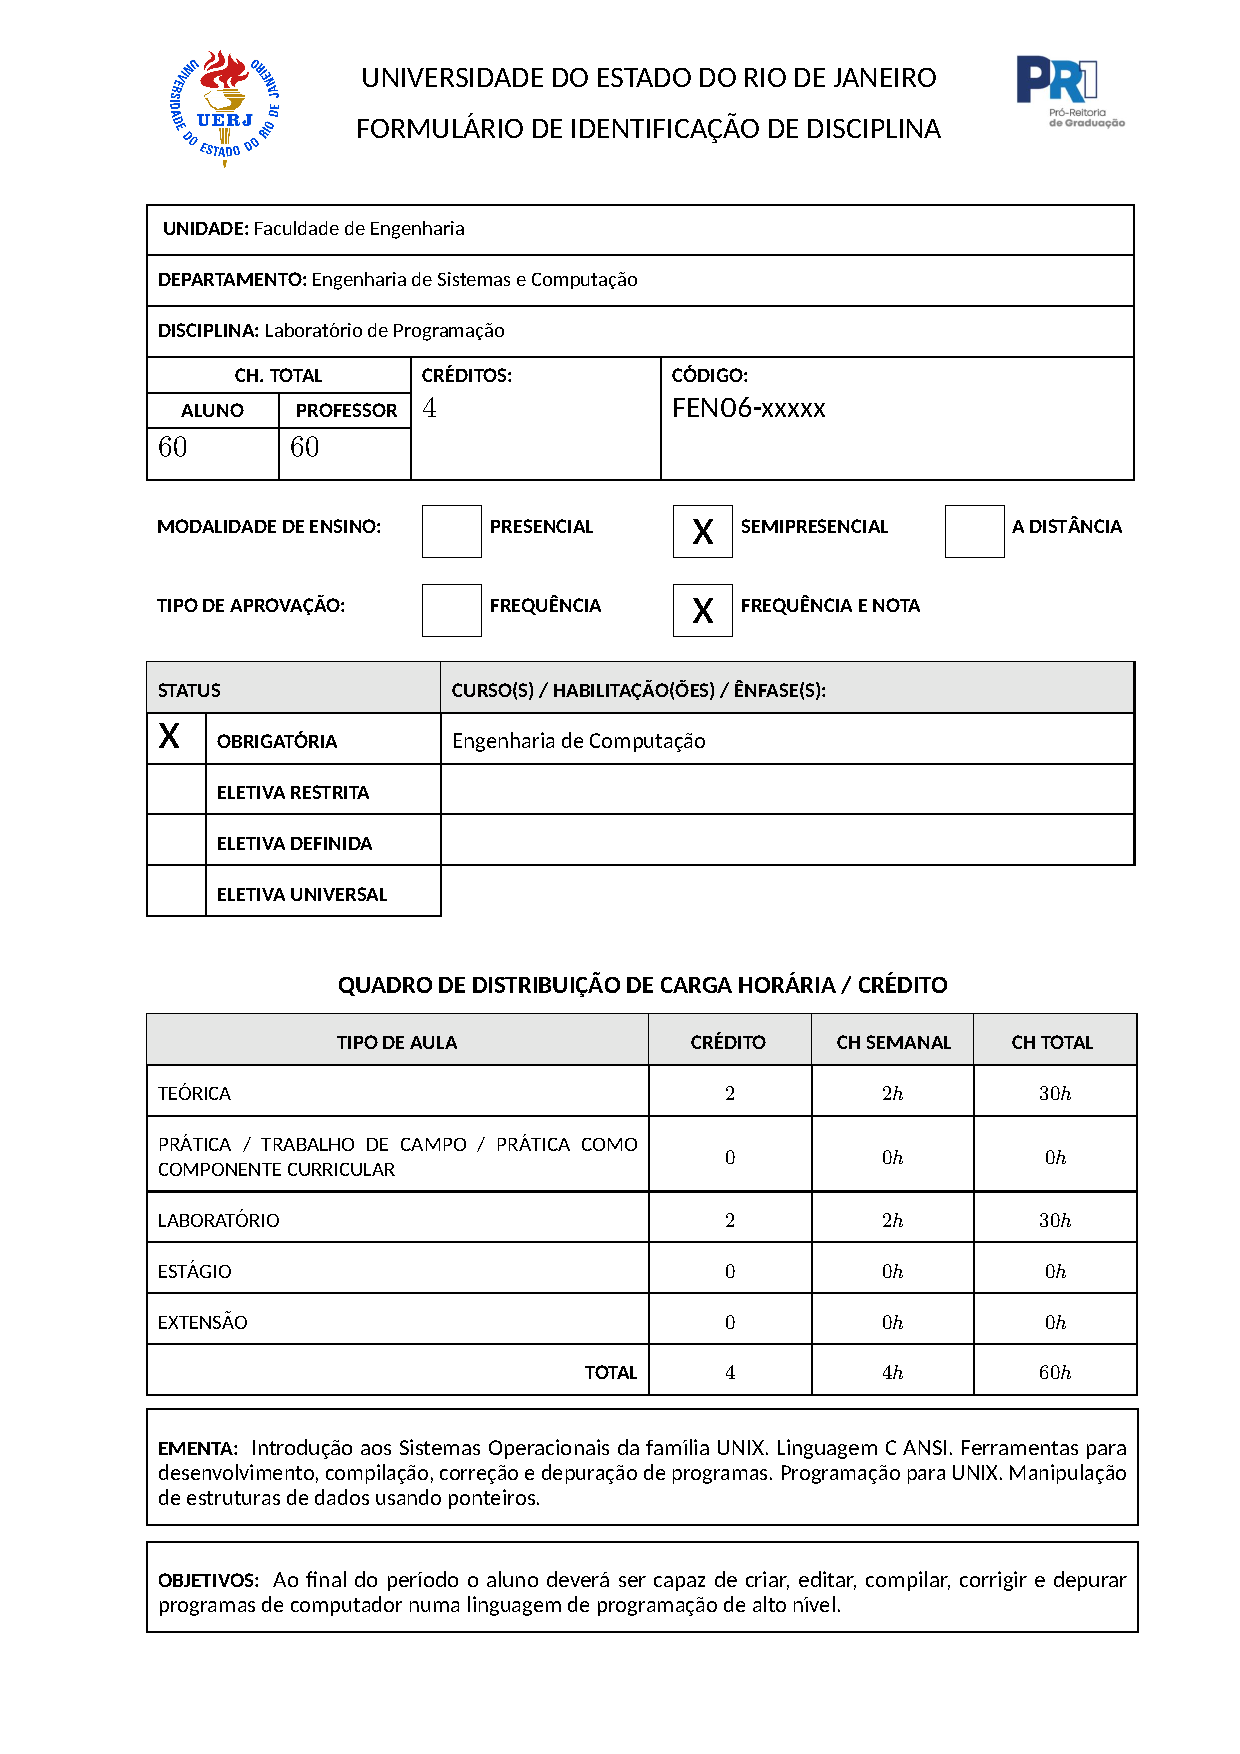
\includepdf[pages=-,addtotoc={1,section,1,{\LabProgA},},pagecommand={\thispagestyle{fancy}}]{ementas/LaboratorioDeProgramacaoA.pdf}
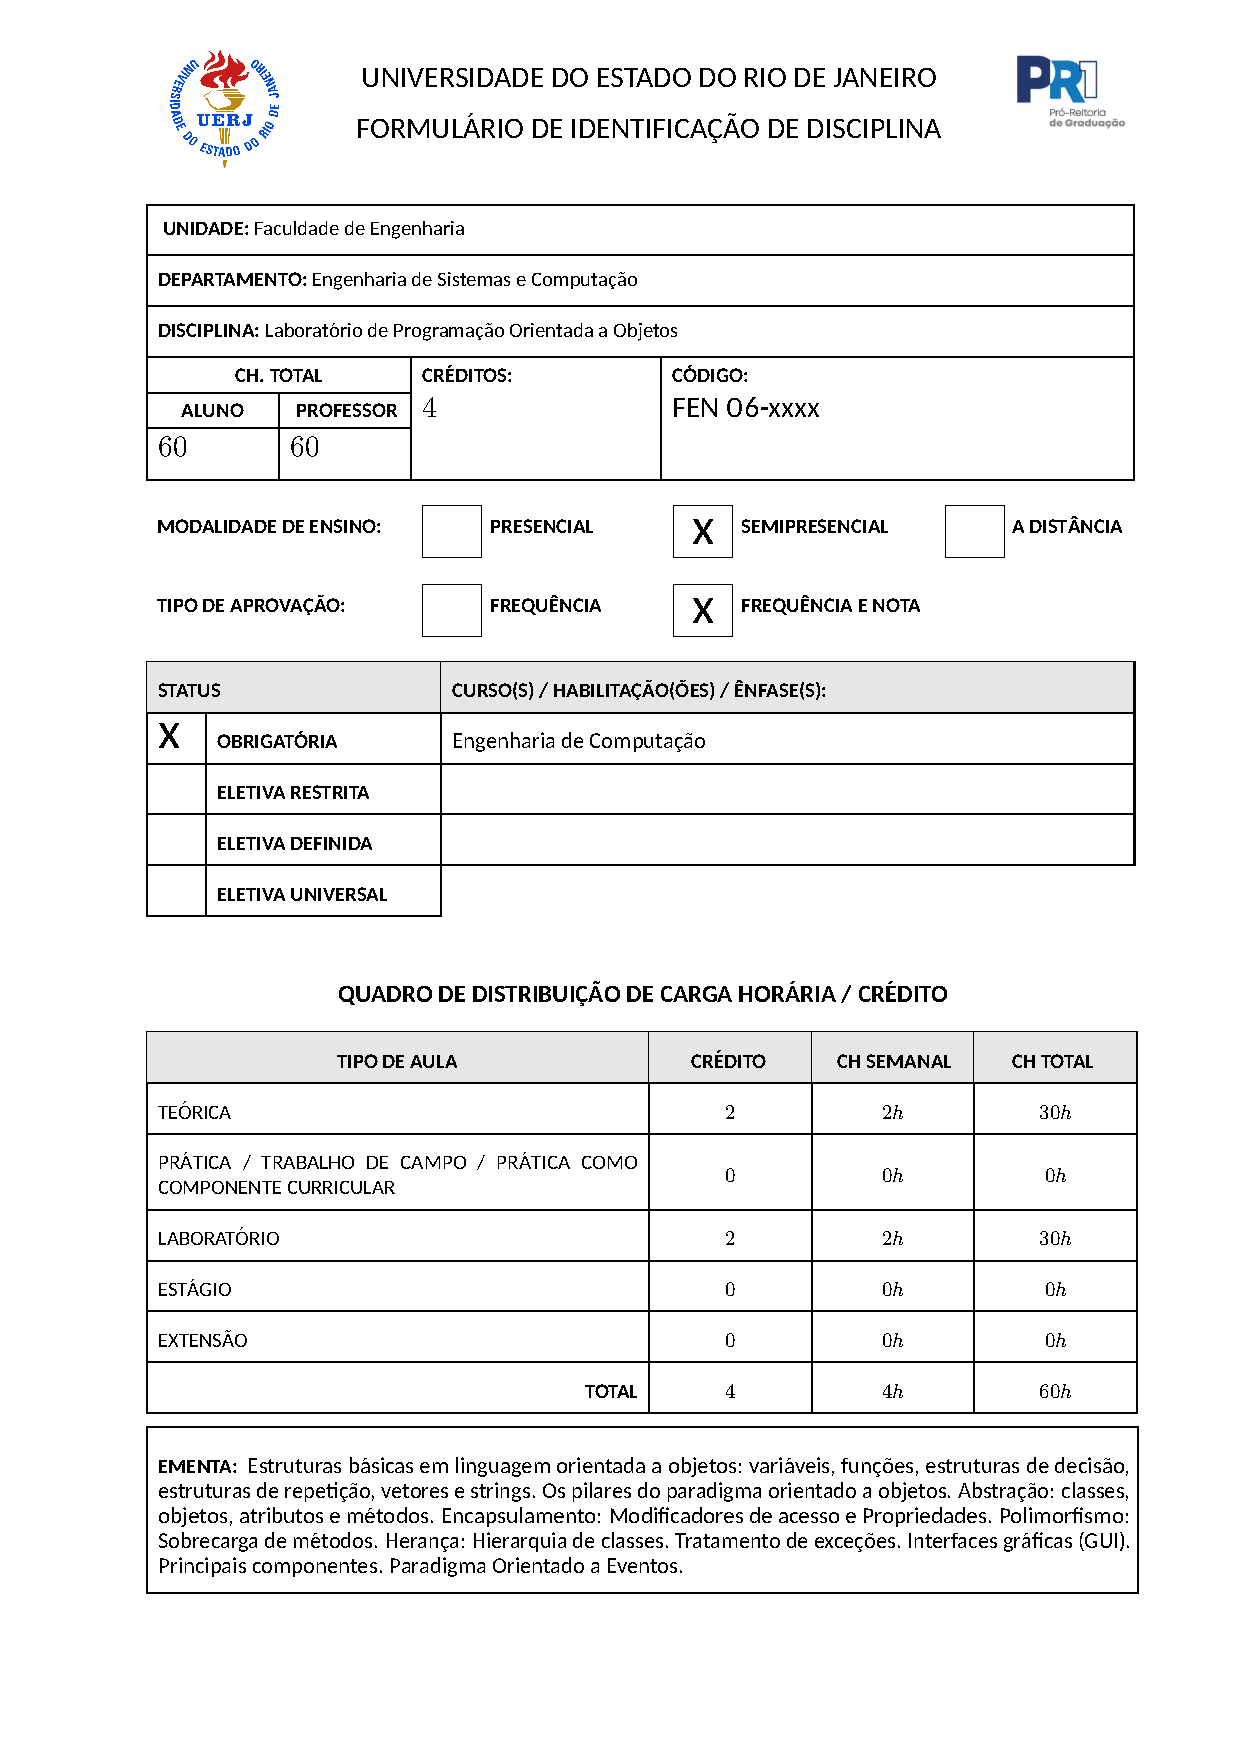
\includepdf[pages=-,addtotoc={1,section,1,{\LabProgPOO},},pagecommand={\thispagestyle{fancy}}]{ementas/LaboratorioDeProgramacaoB.pdf}
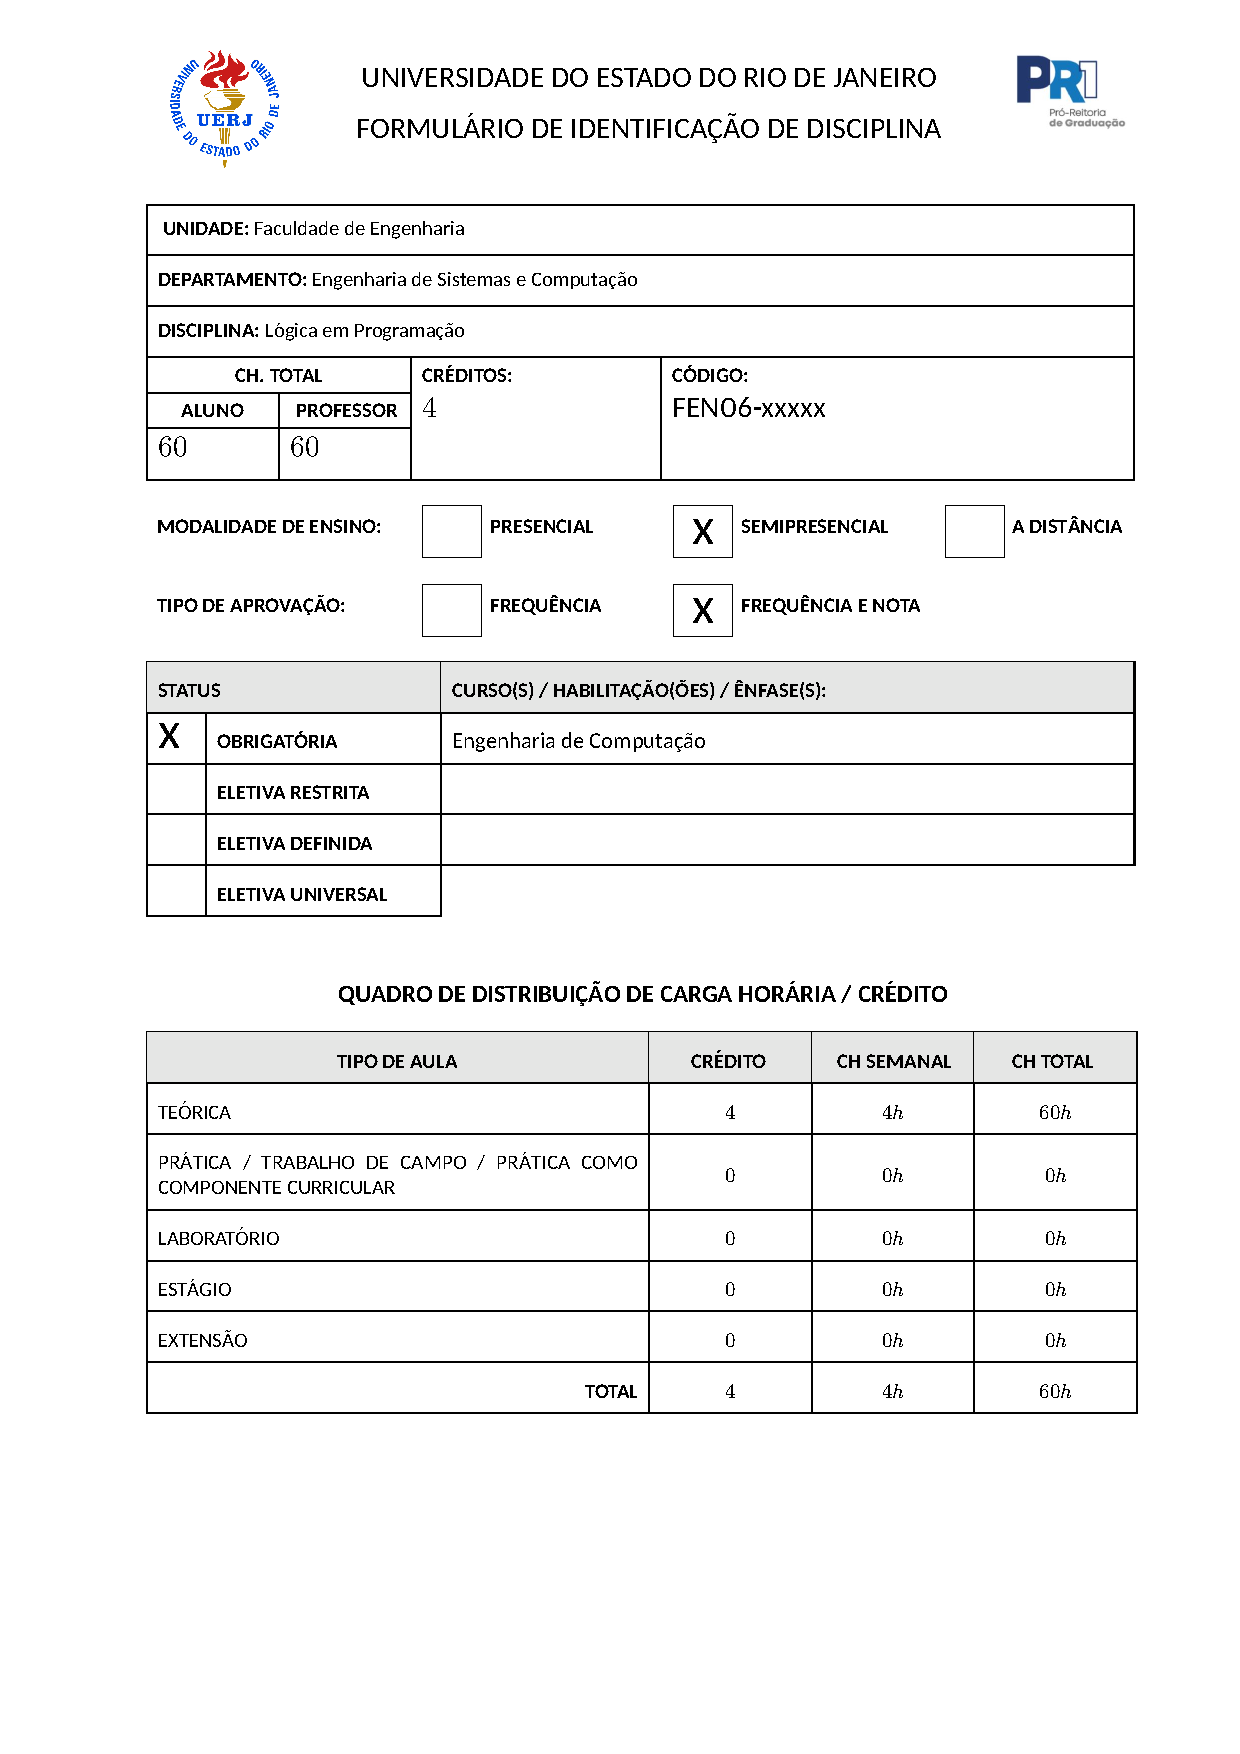
\includepdf[pages=-,addtotoc={1,section,1,{\LogProg},},pagecommand={\thispagestyle{fancy}}]{ementas/LogicaEmProgramacao.pdf}
\includepdf[pages=-,addtotoc={1,section,1,{\MacroEco},},pagecommand={\thispagestyle{fancy}}]{ementasExternas/macroeconomia.pdf} % Macroeconomia
% Materiais Elétricos e Eletrônicos era 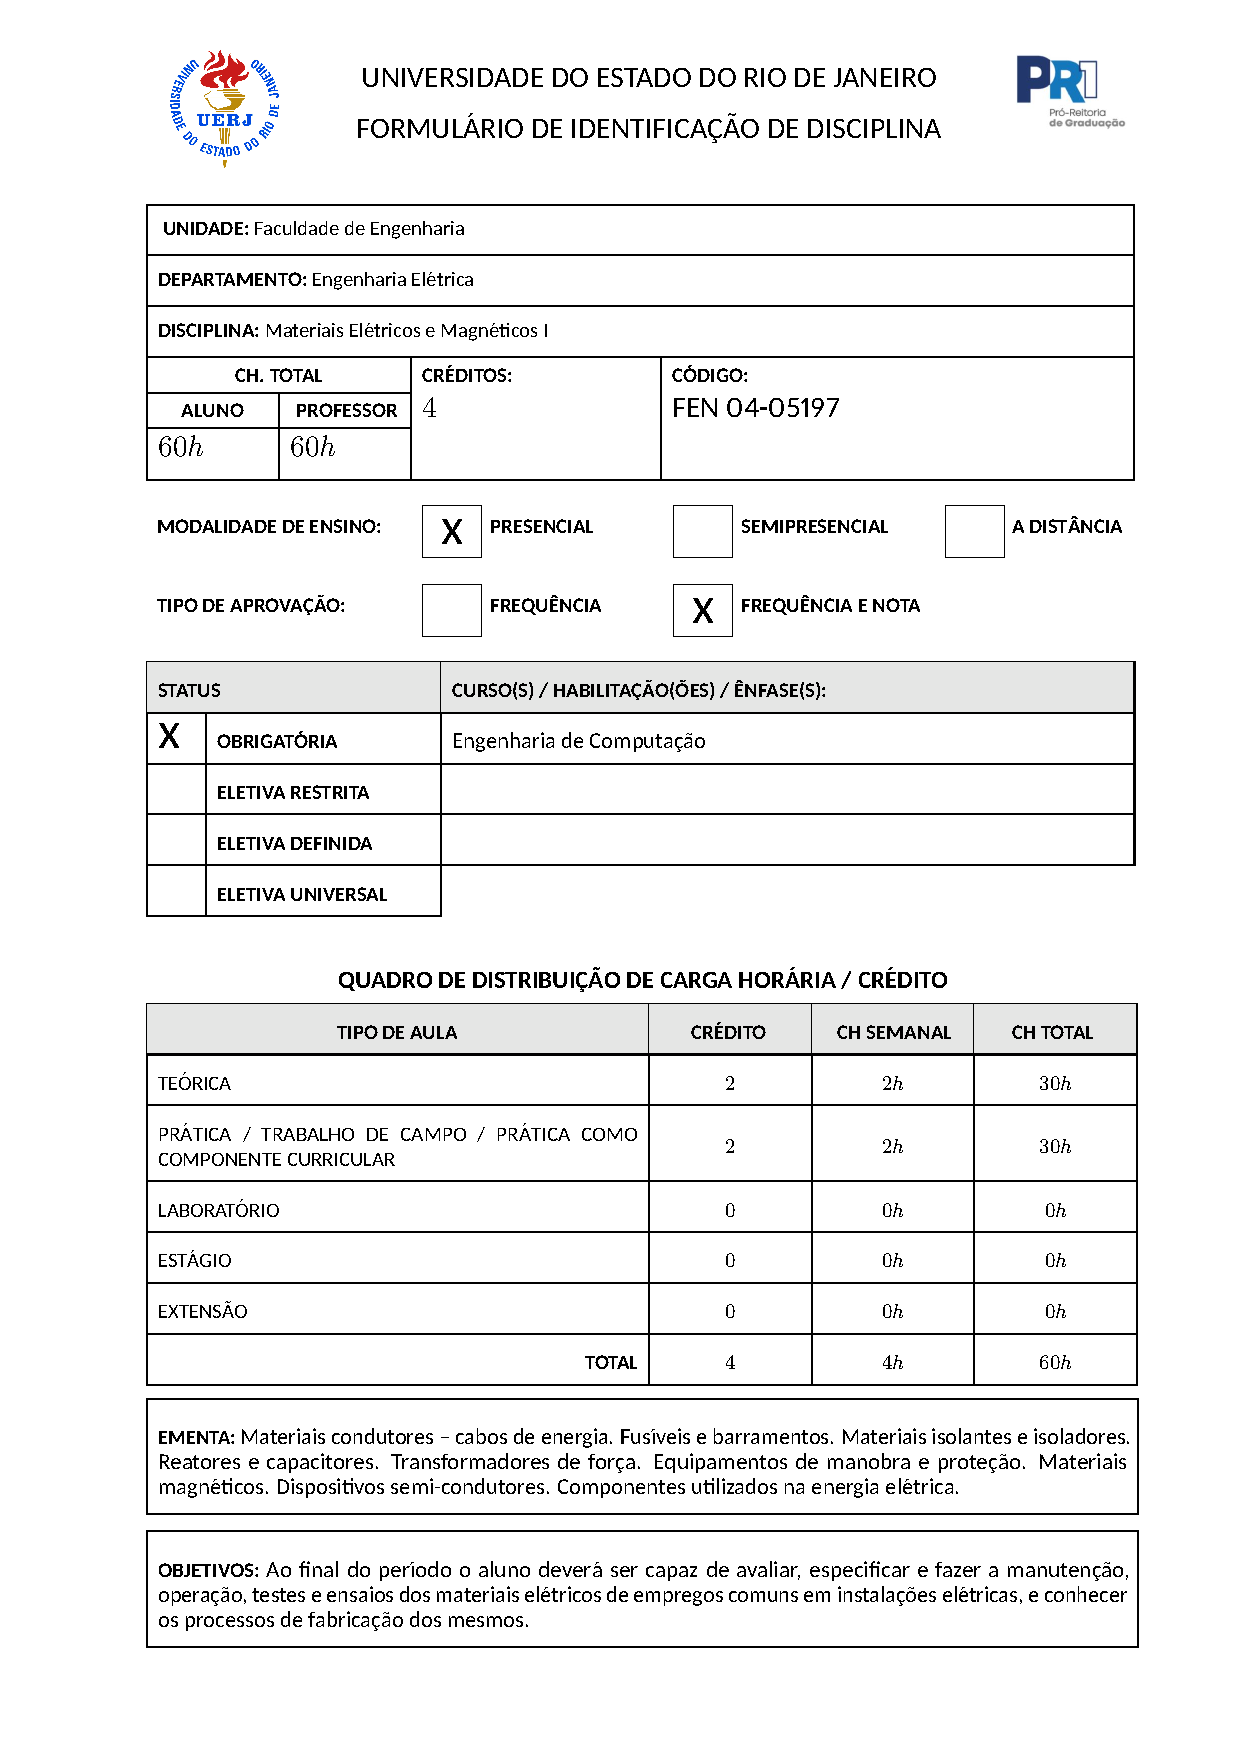
\includepdf[pages=-,addtotoc={1,section,1,{\MatEle},},pagecommand={\thispagestyle{fancy}}]{ementas/MateriaisEletricosEMagneticos.pdf}
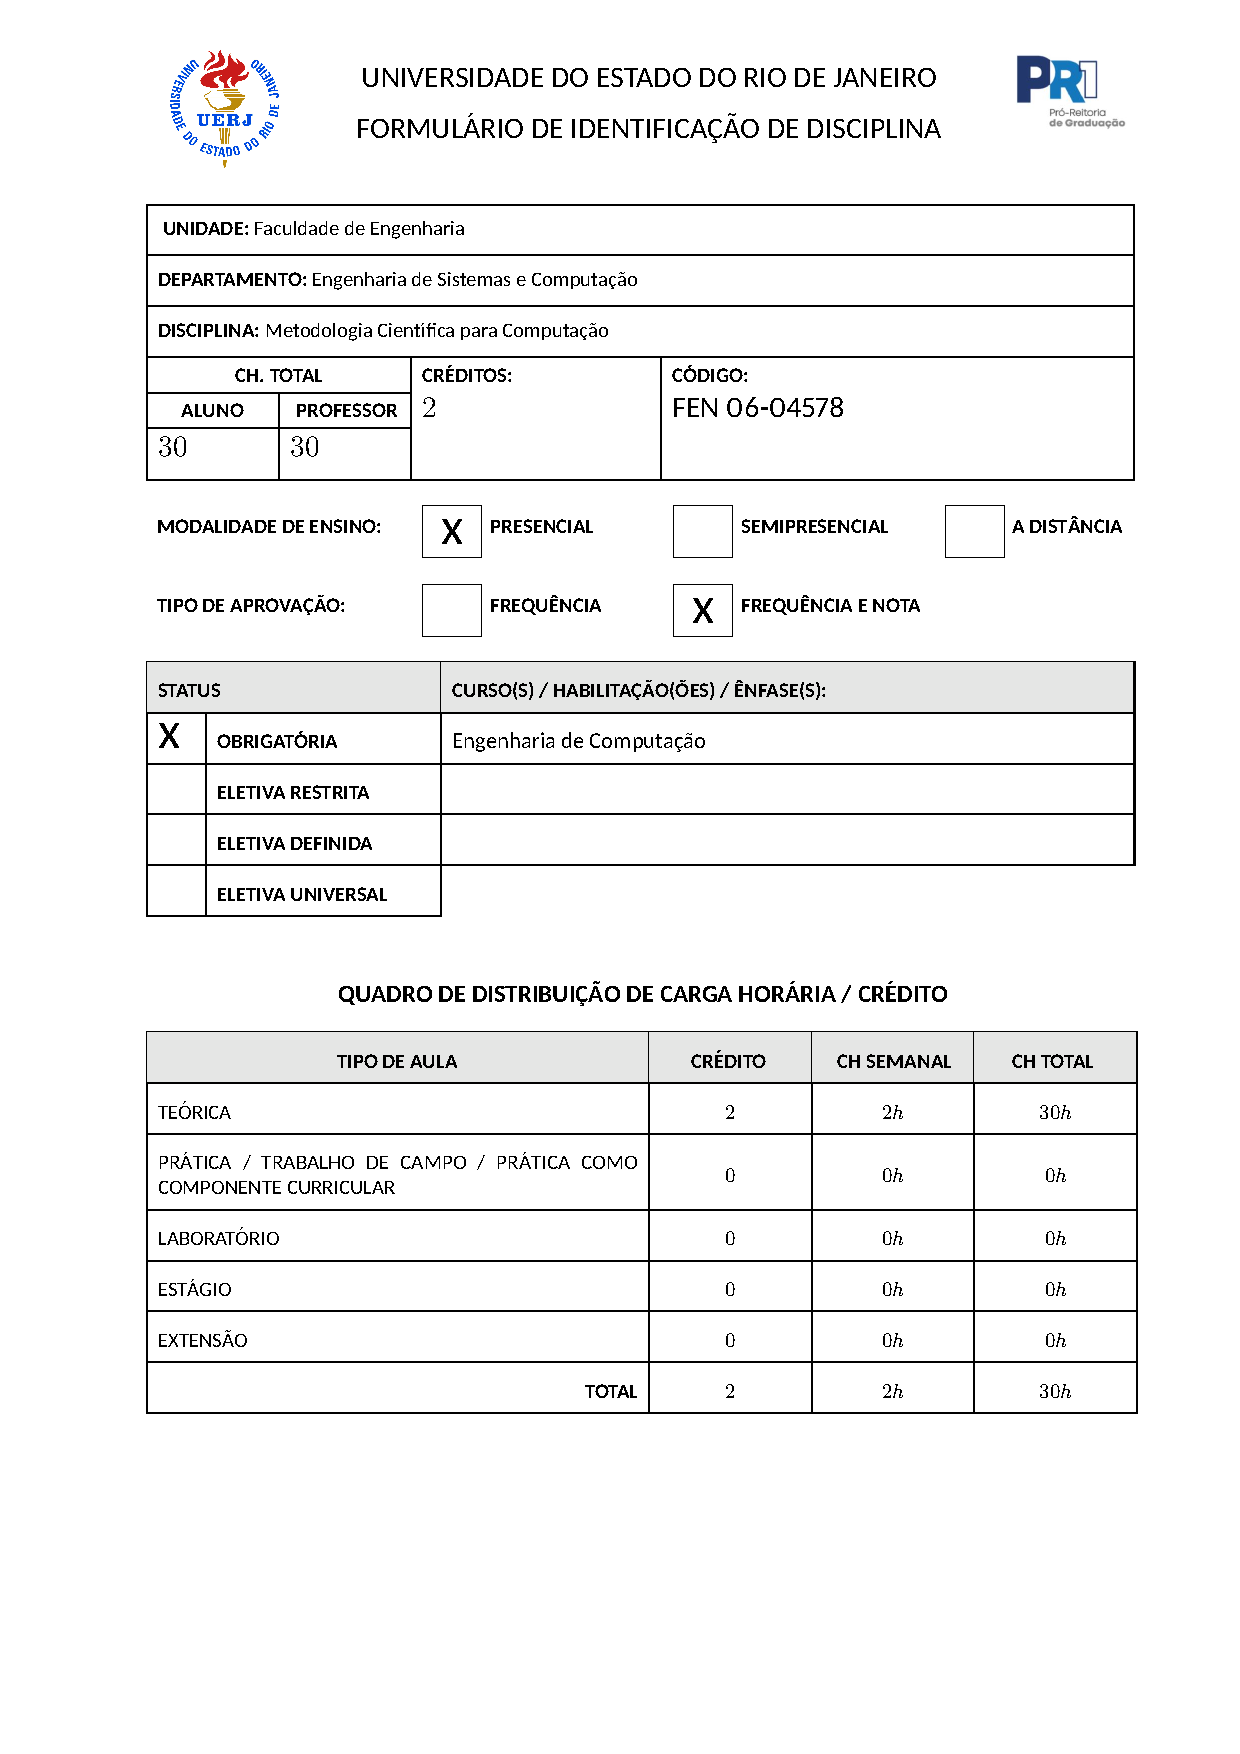
\includepdf[pages=-,addtotoc={1,section,1,{\ProjA},},pagecommand={\thispagestyle{fancy}}]{ementas/ProjetoXIA.pdf} %  Metodo de Projeto 
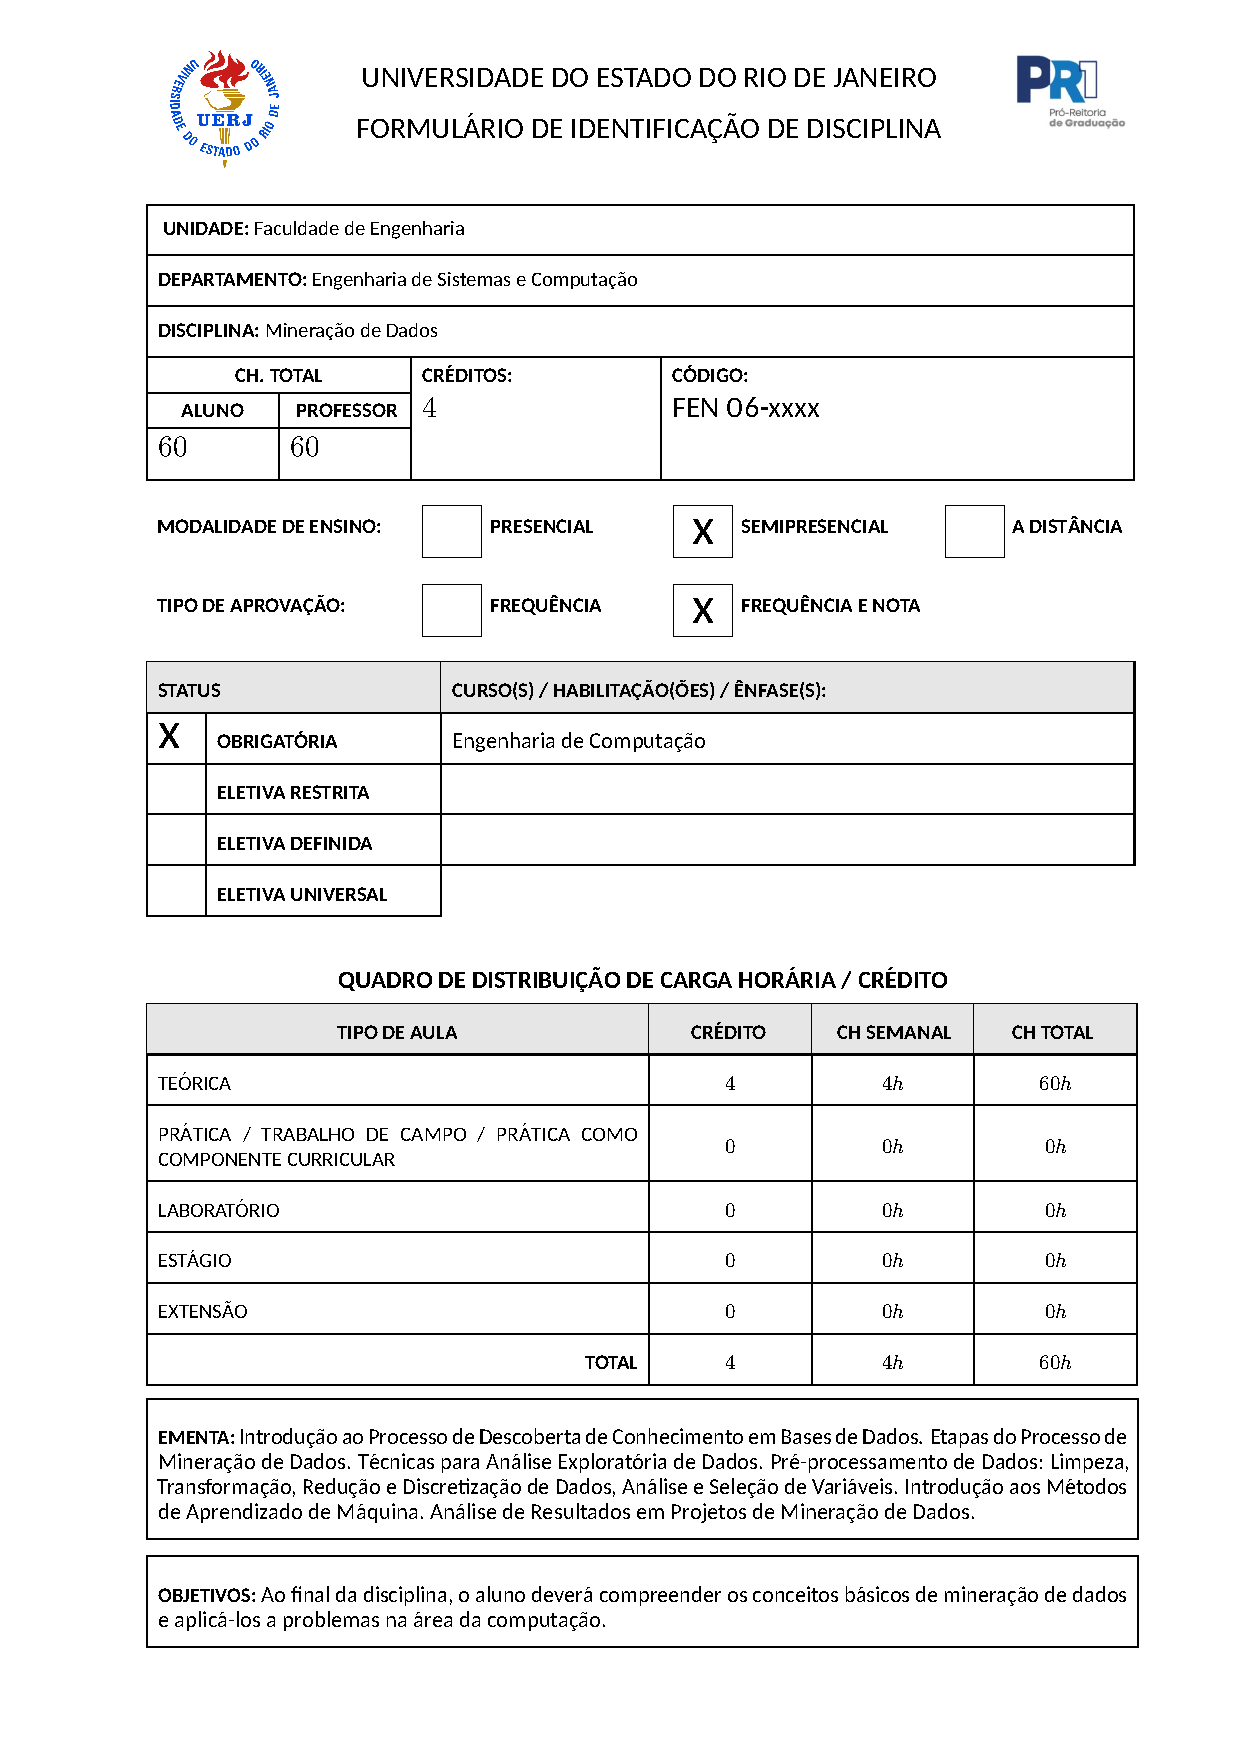
\includepdf[pages=-,addtotoc={1,section,1,{\MineraDados},},pagecommand={\thispagestyle{fancy}}]{ementas/MineracaoDeDados.pdf}
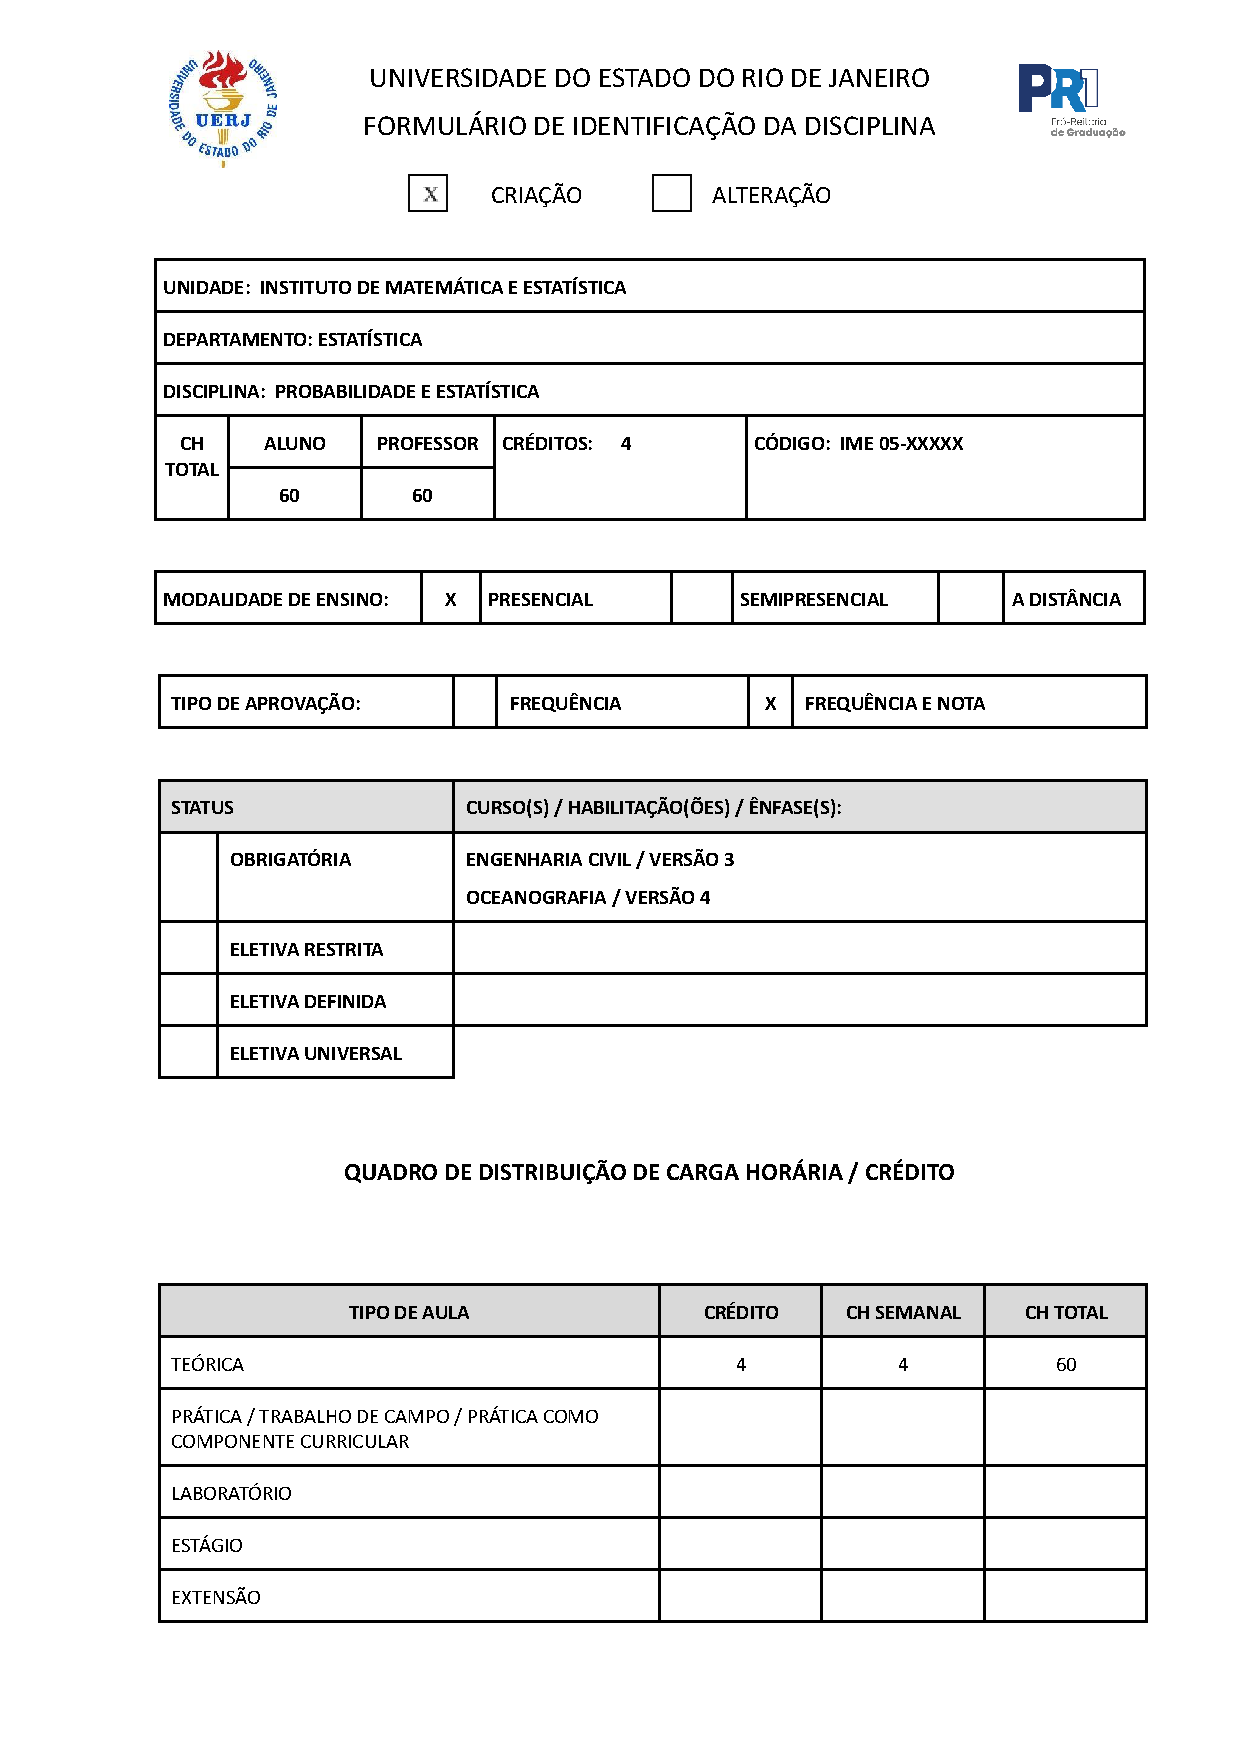
\includepdf[pages=-,addtotoc={1,section,1,{\ProbEst},},pagecommand={\thispagestyle{fancy}}]{ementasExternas/Probabilidade_e_Estatistica.pdf}
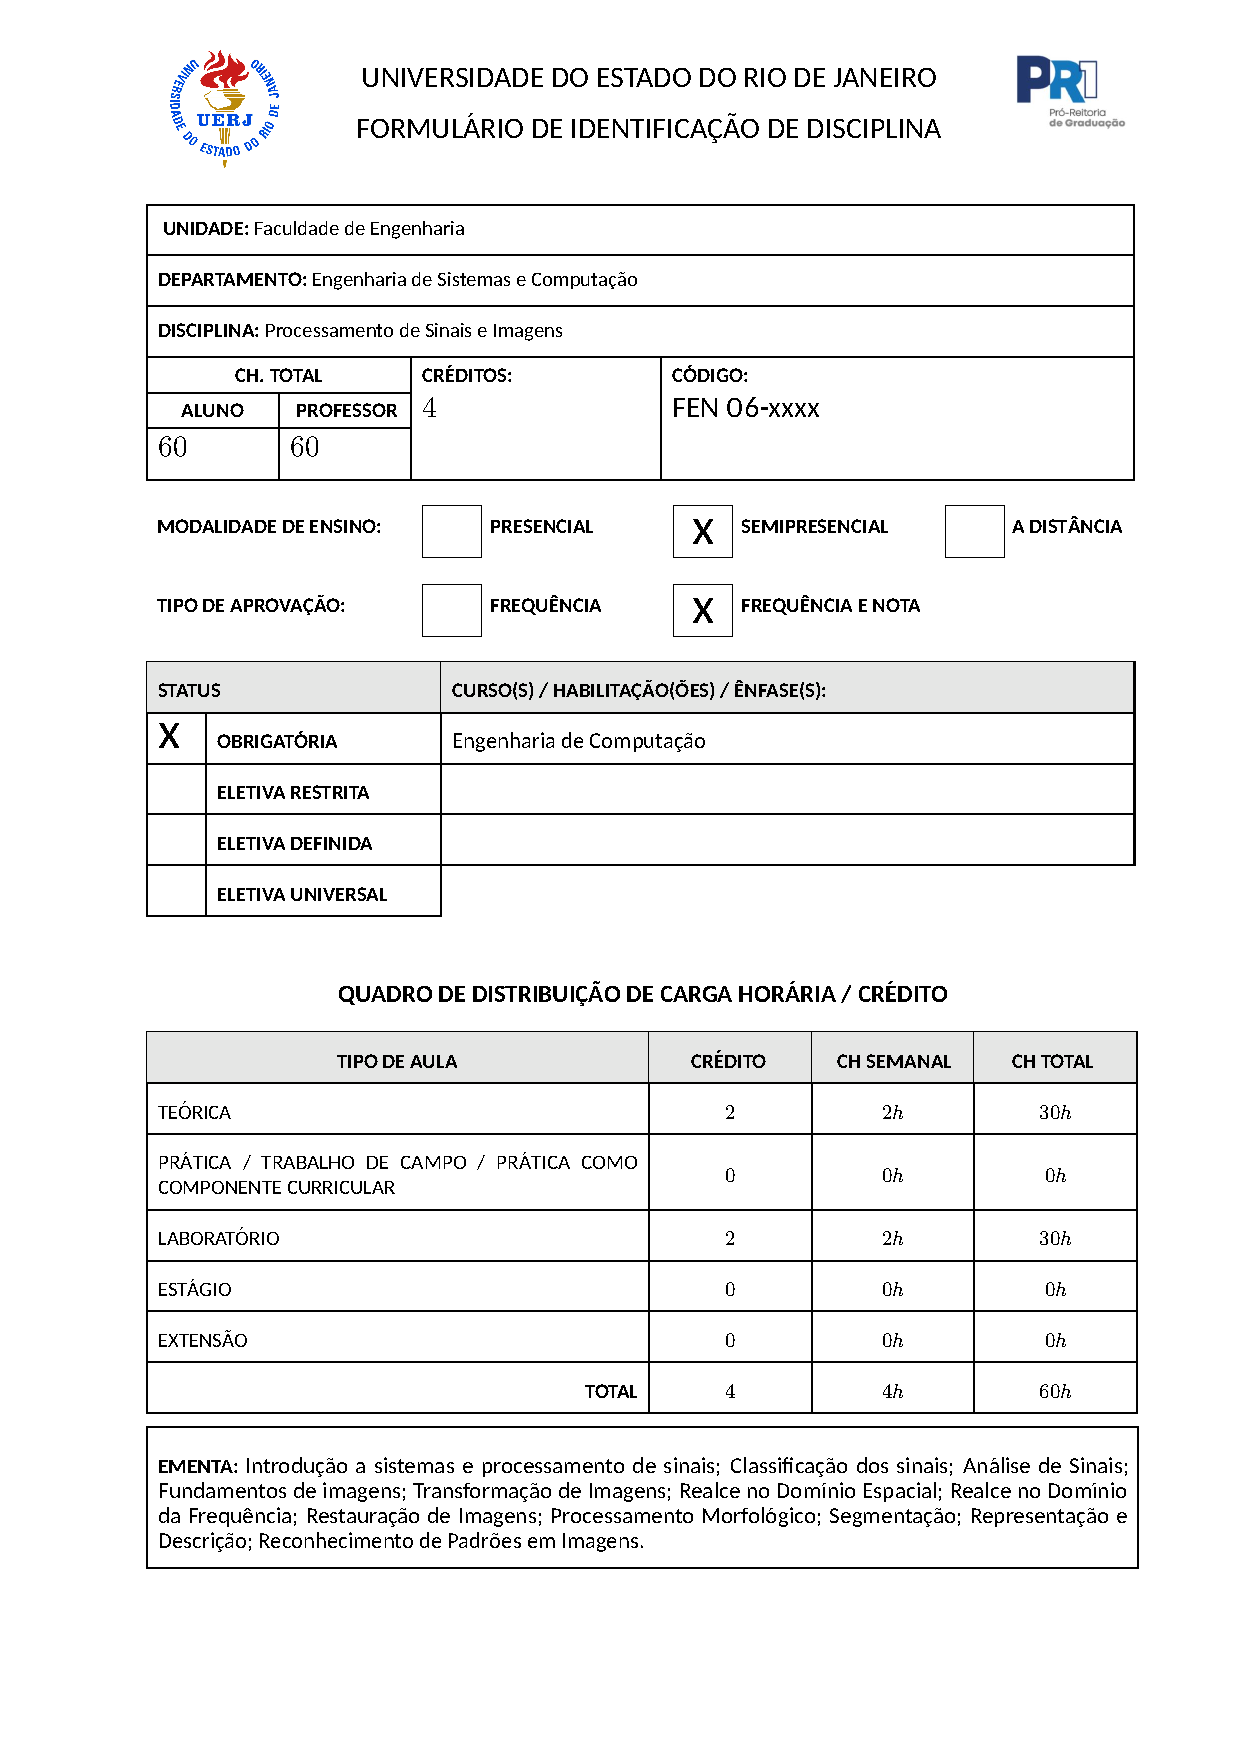
\includepdf[pages=-,addtotoc={1,section,1,{\ProcImag},},pagecommand={\thispagestyle{fancy}}]{ementas/ProcessamentoDeImagens.pdf}
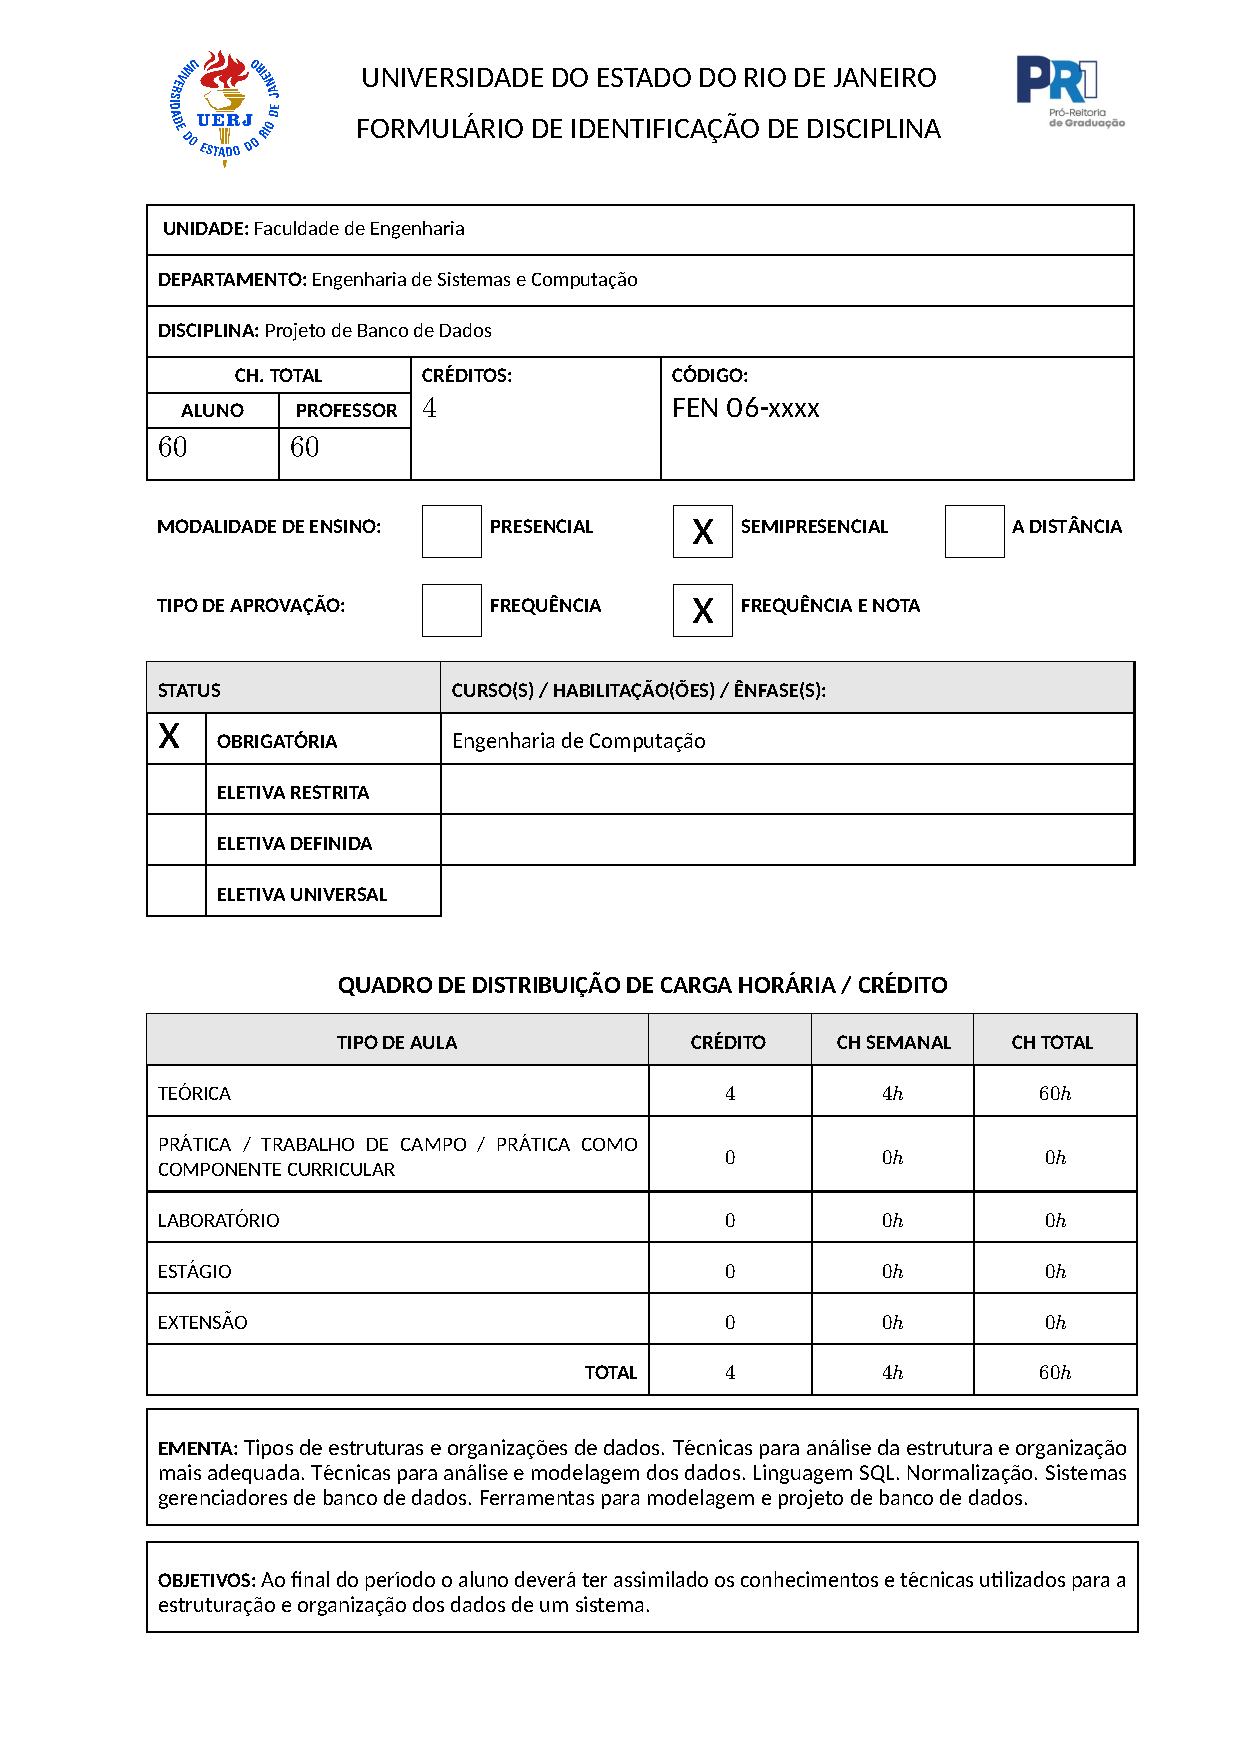
\includepdf[pages=-,addtotoc={1,section,1,{\ProjBD},},pagecommand={\thispagestyle{fancy}}]{ementas/ProjetoEAdministracaoDeBancoDeDados.pdf}
% Projetos de Extensão
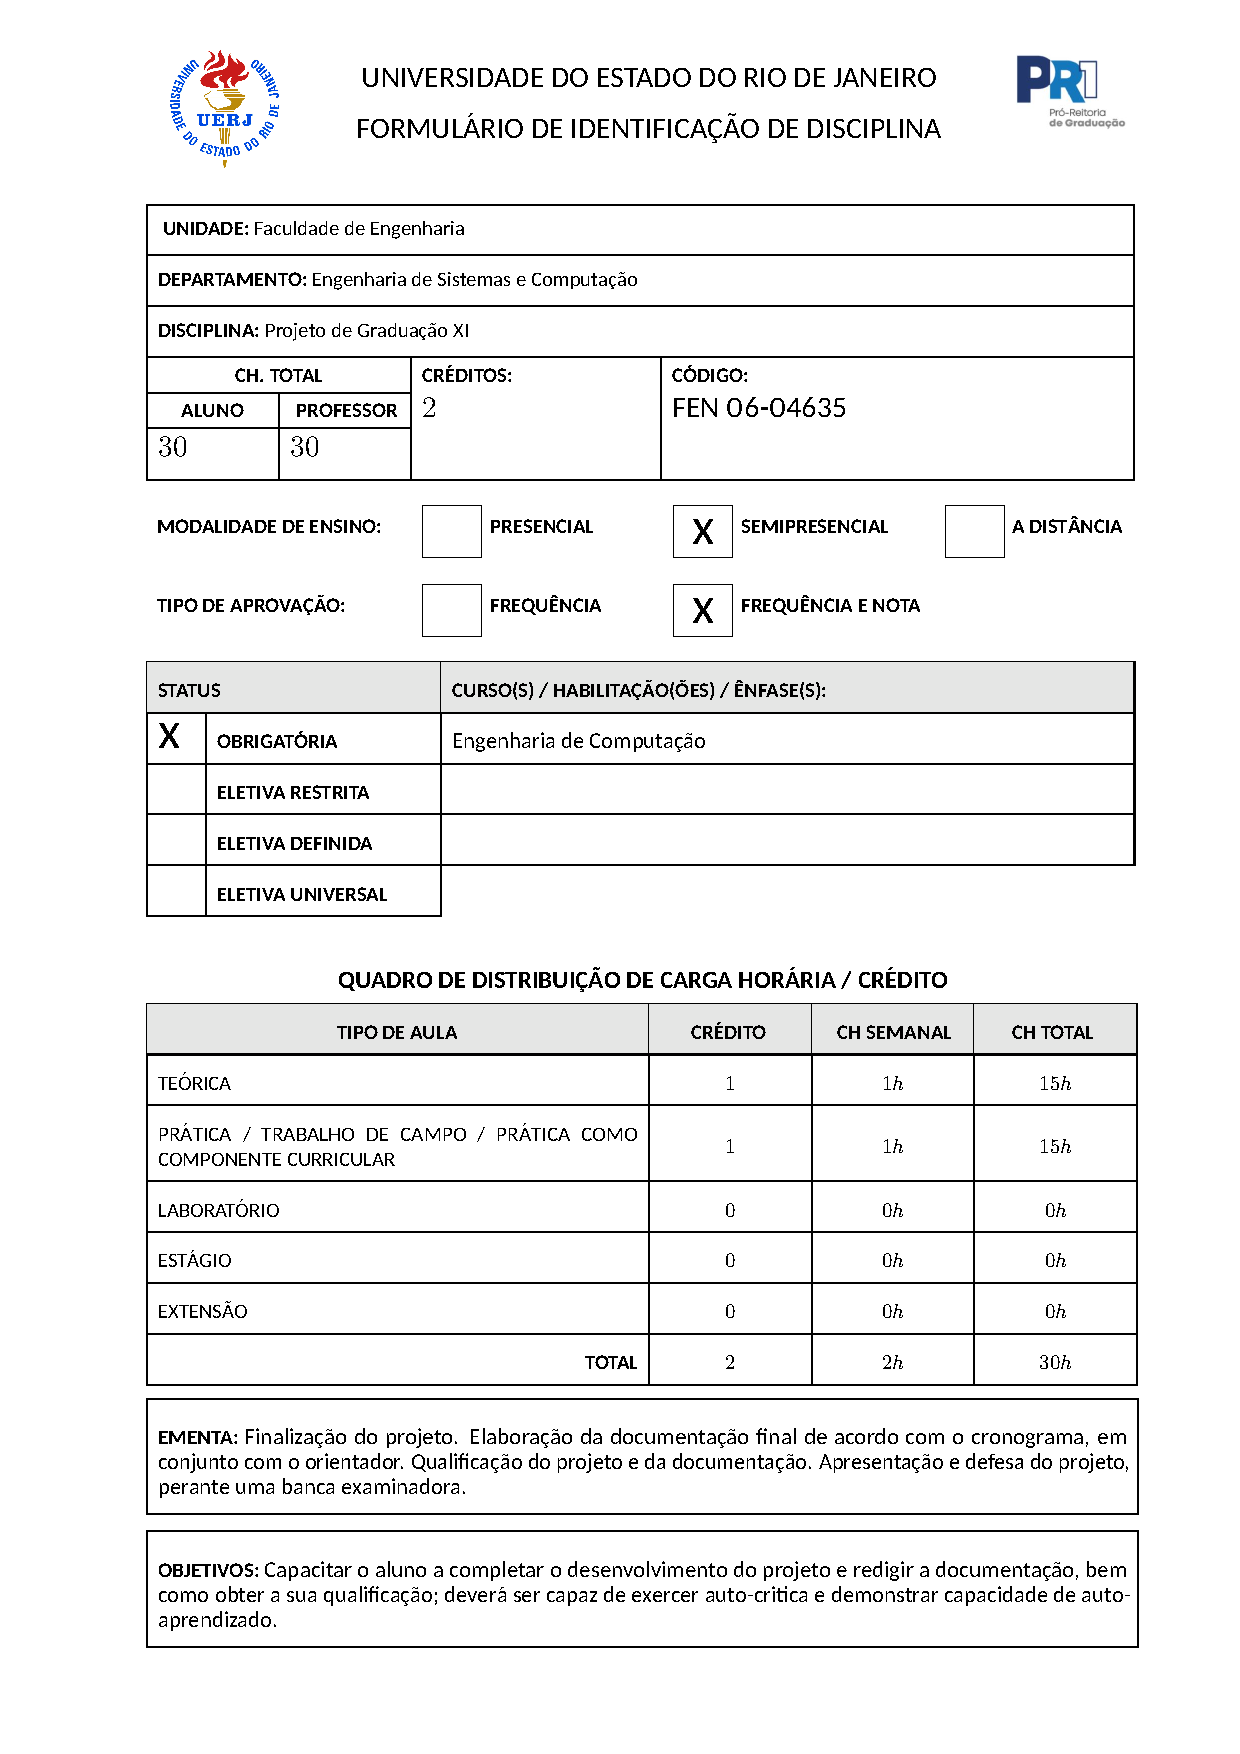
\includepdf[pages=-,addtotoc={1,section,1,{\ProjB},},pagecommand={\thispagestyle{fancy}}]{ementas/ProjetoXIB.pdf}
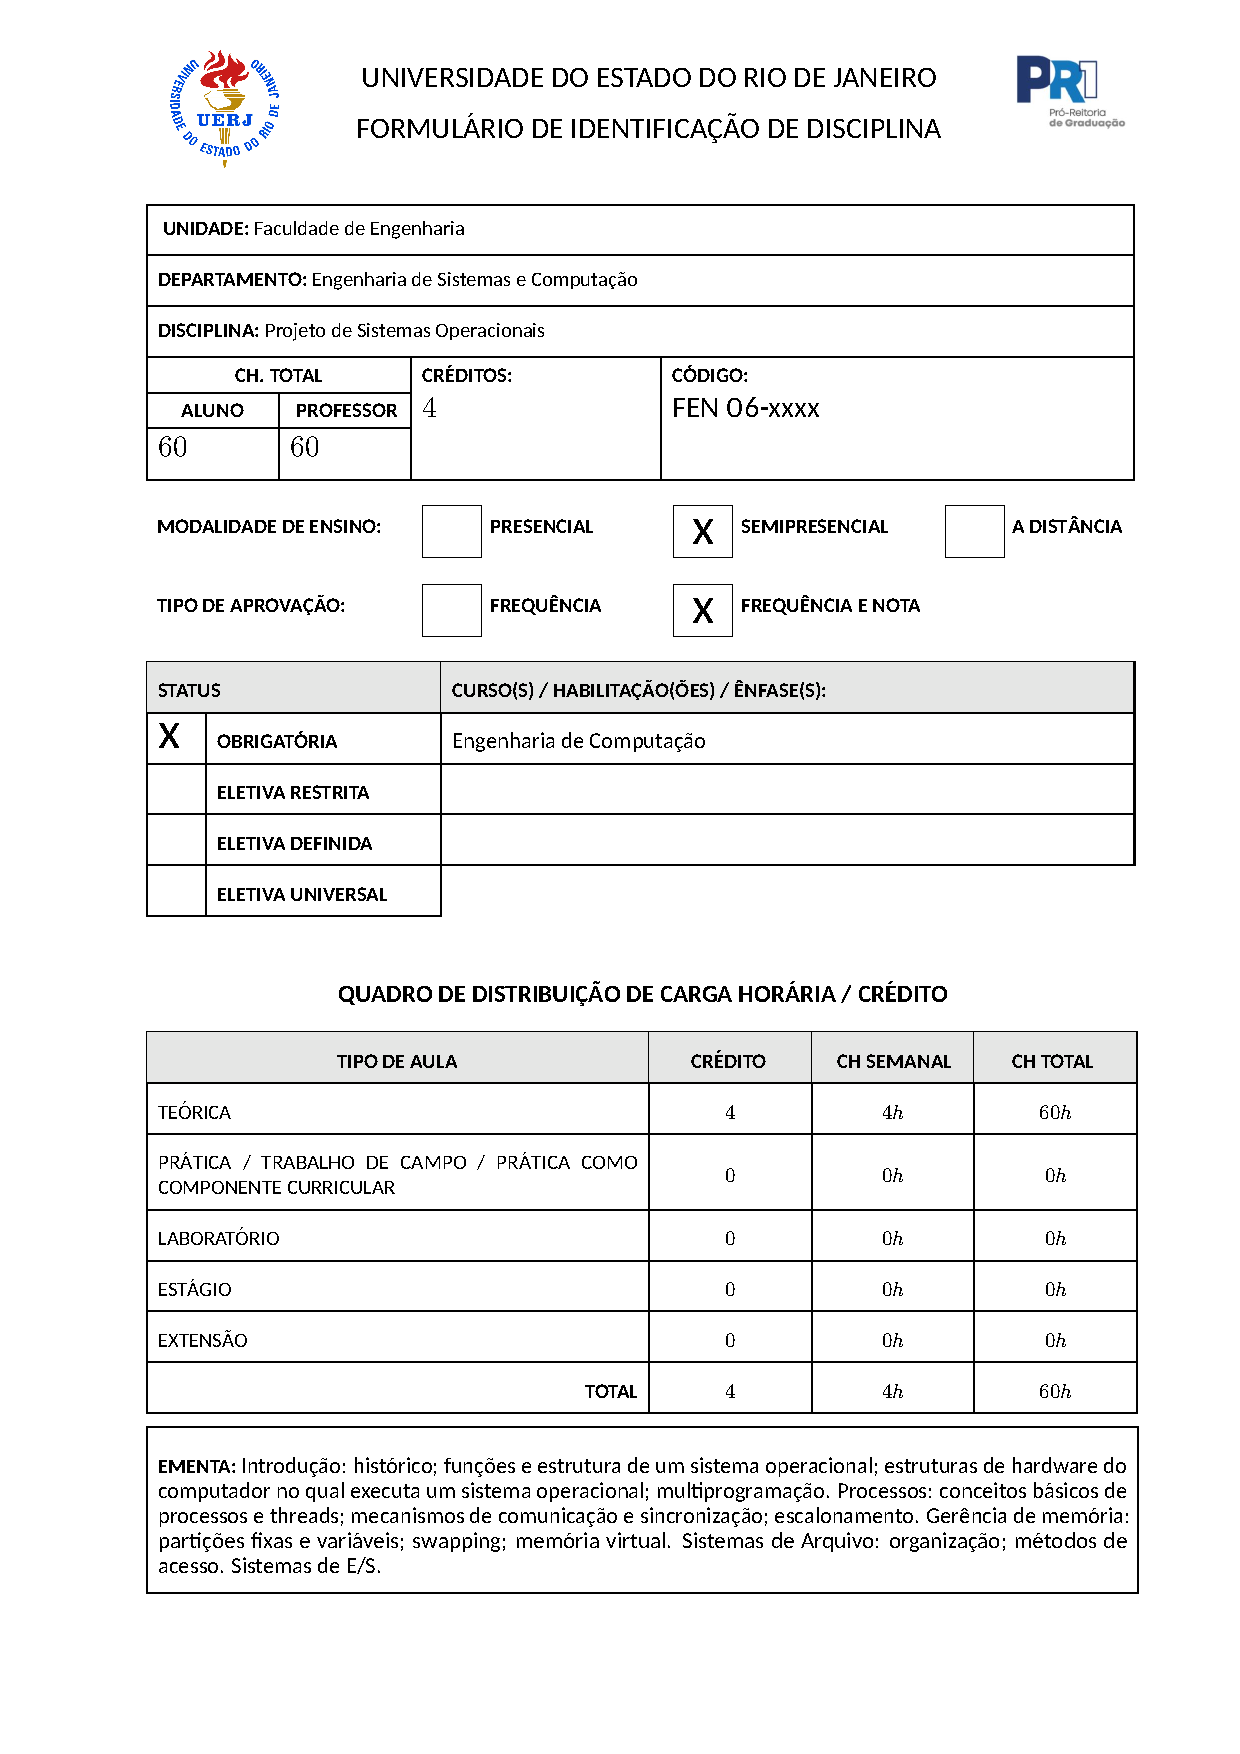
\includepdf[pages=-,addtotoc={1,section,1,{\ProjSO},},pagecommand={\thispagestyle{fancy}}]{ementas/ProjetoDeSistemasOperacionais.pdf}
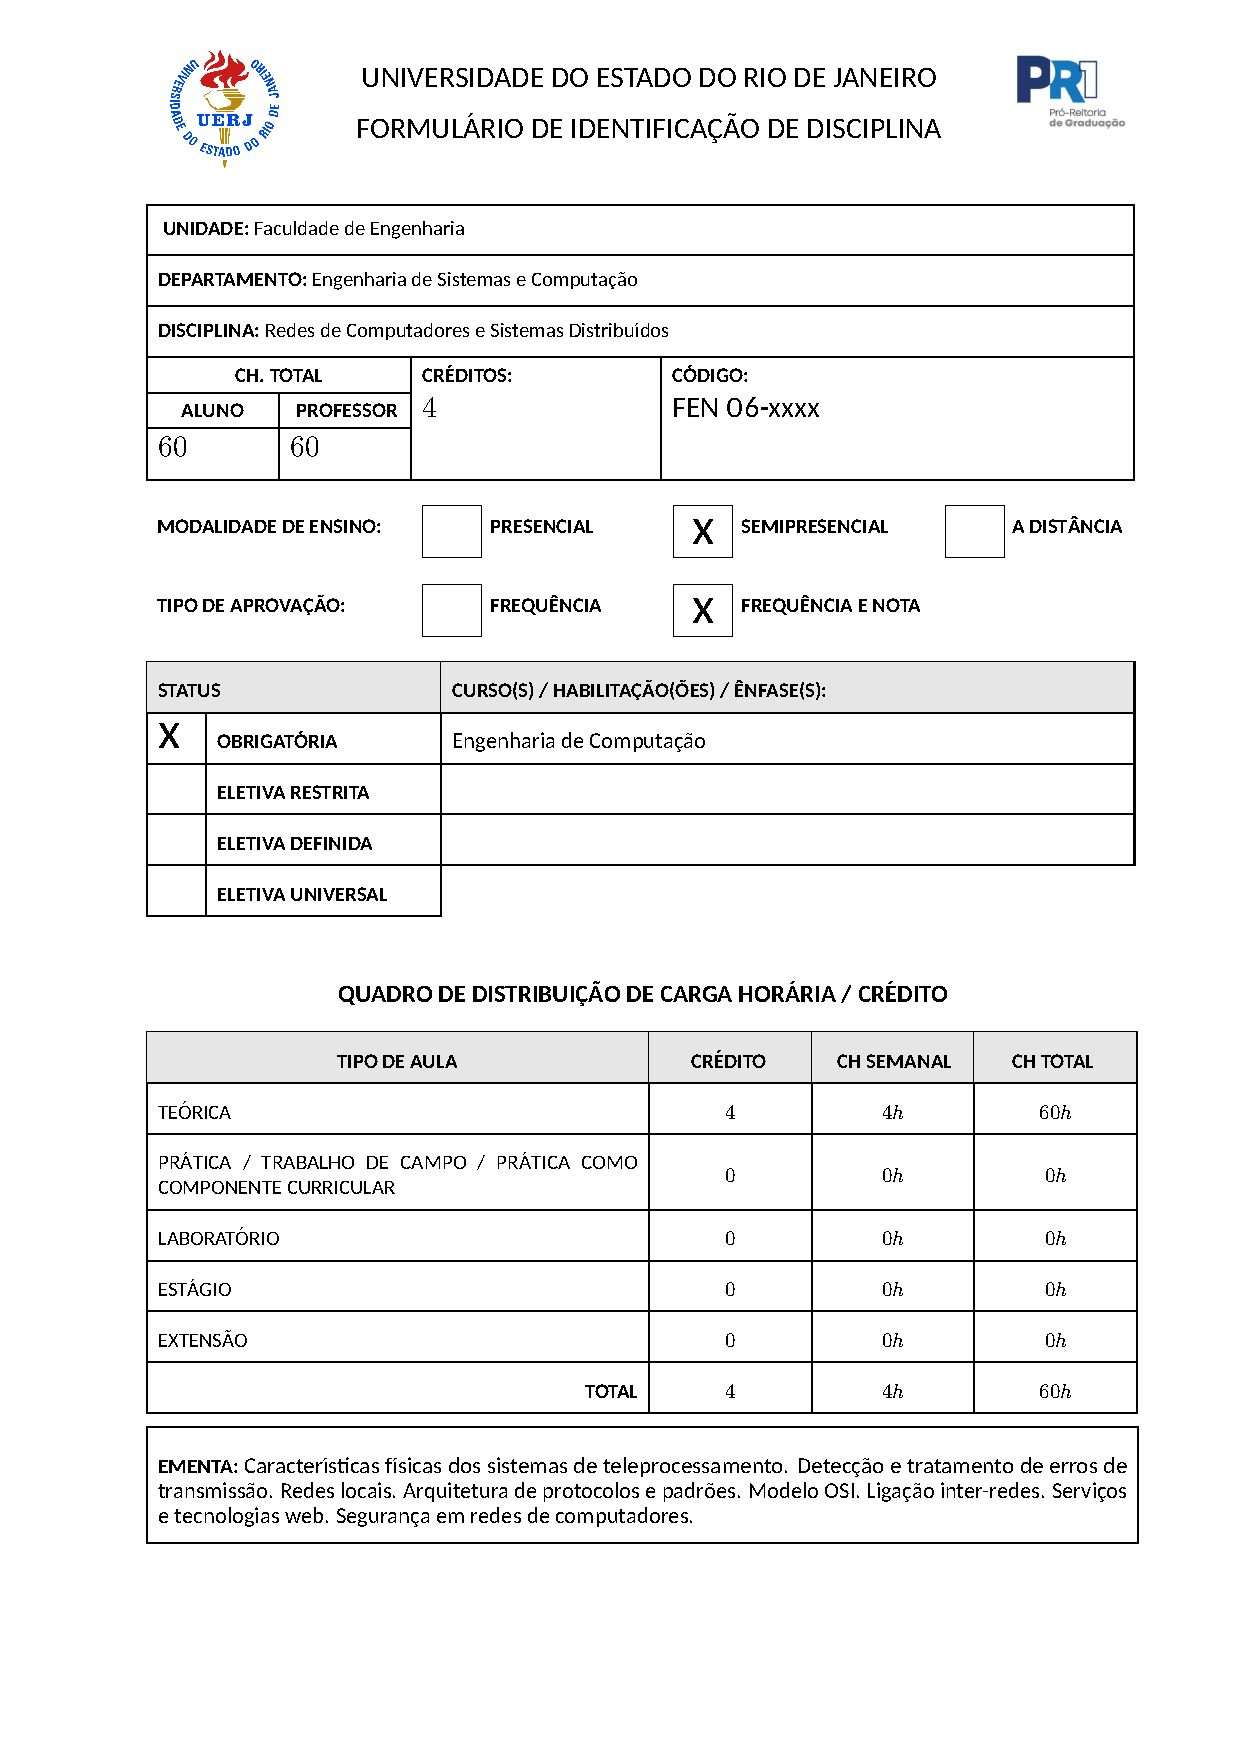
\includepdf[pages=-,addtotoc={1,section,1,{\Telep},},pagecommand={\thispagestyle{fancy}}]{ementas/TeleprocessamentoERedes.pdf} % Redes de Computadores e Sistemas Distribuídos
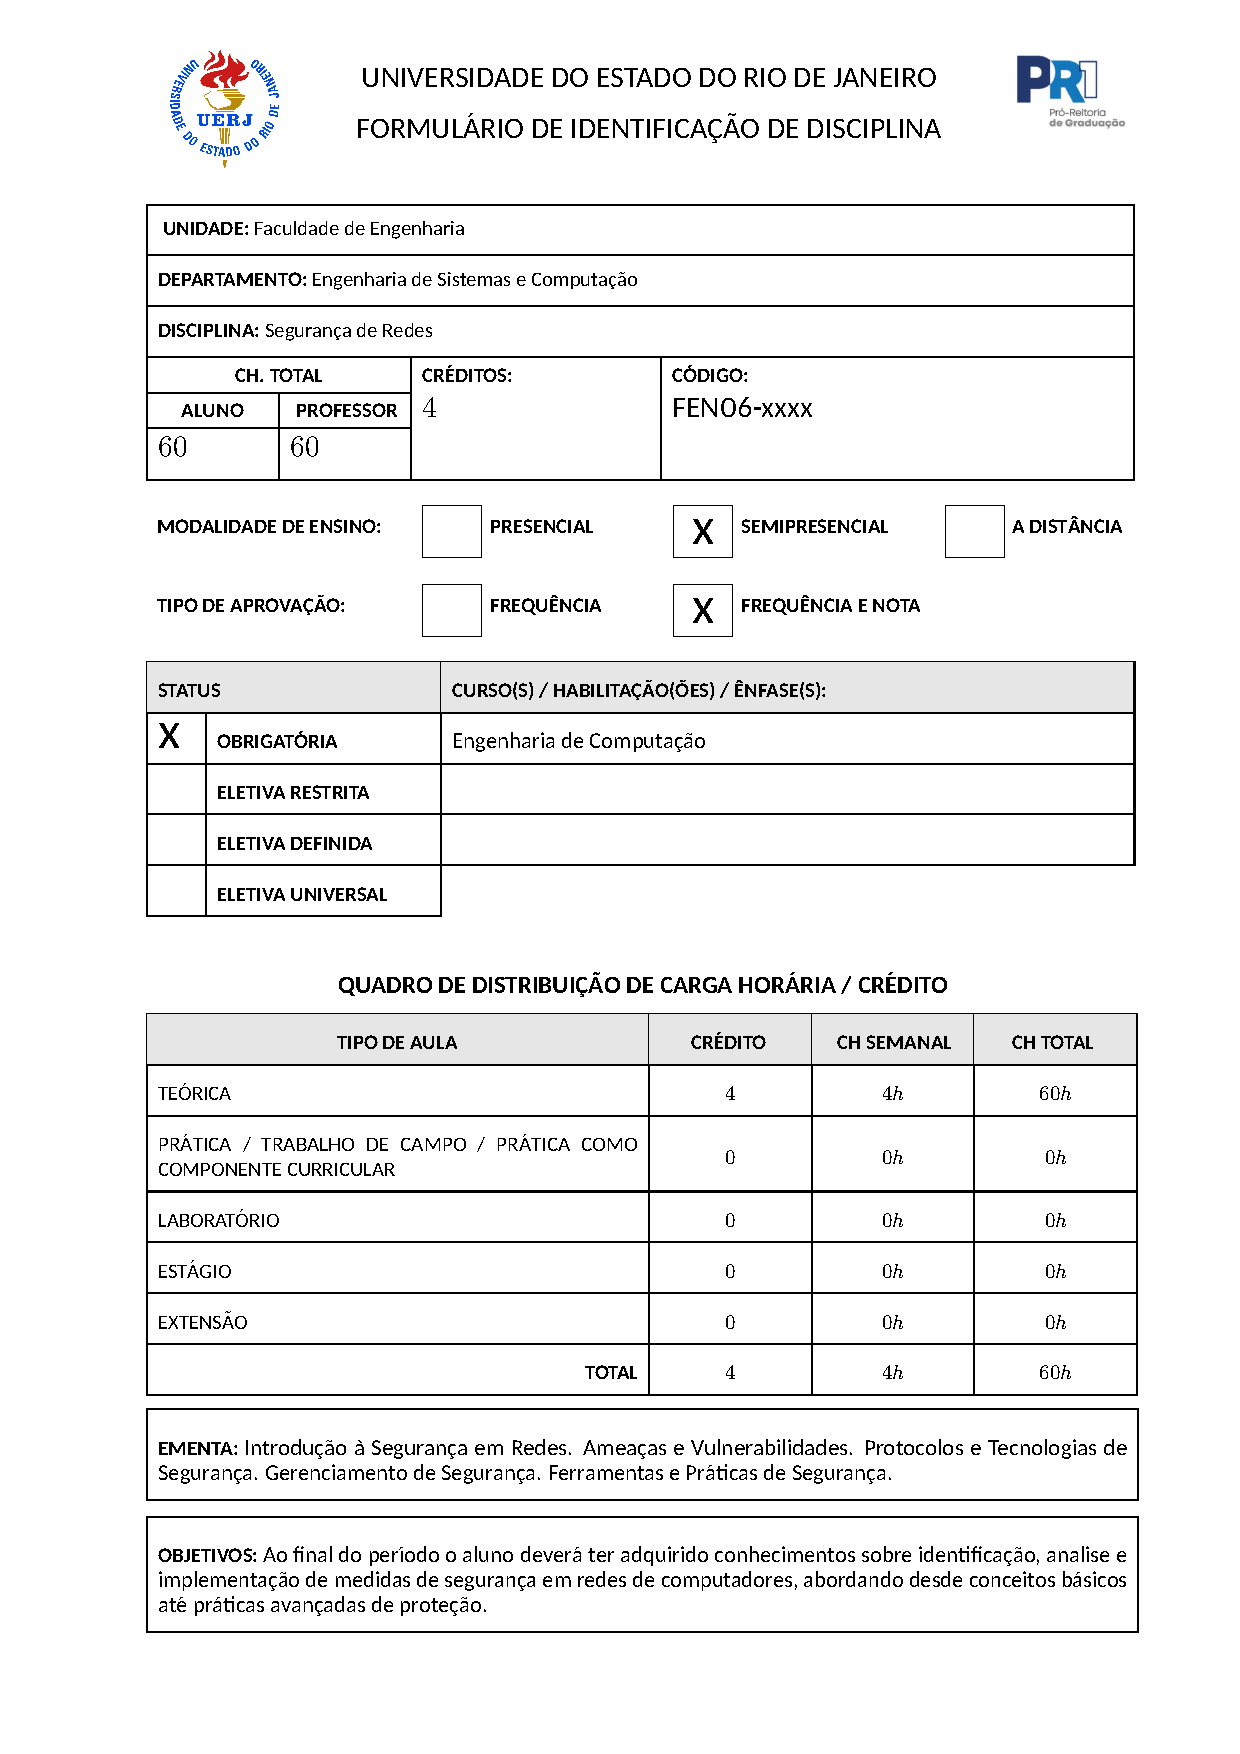
\includepdf[pages=-,addtotoc={1,section,1,{\Sredes},},pagecommand={\thispagestyle{fancy}}]{ementas/seguranca_de_redes.pdf}
% Sinais e Sistemas
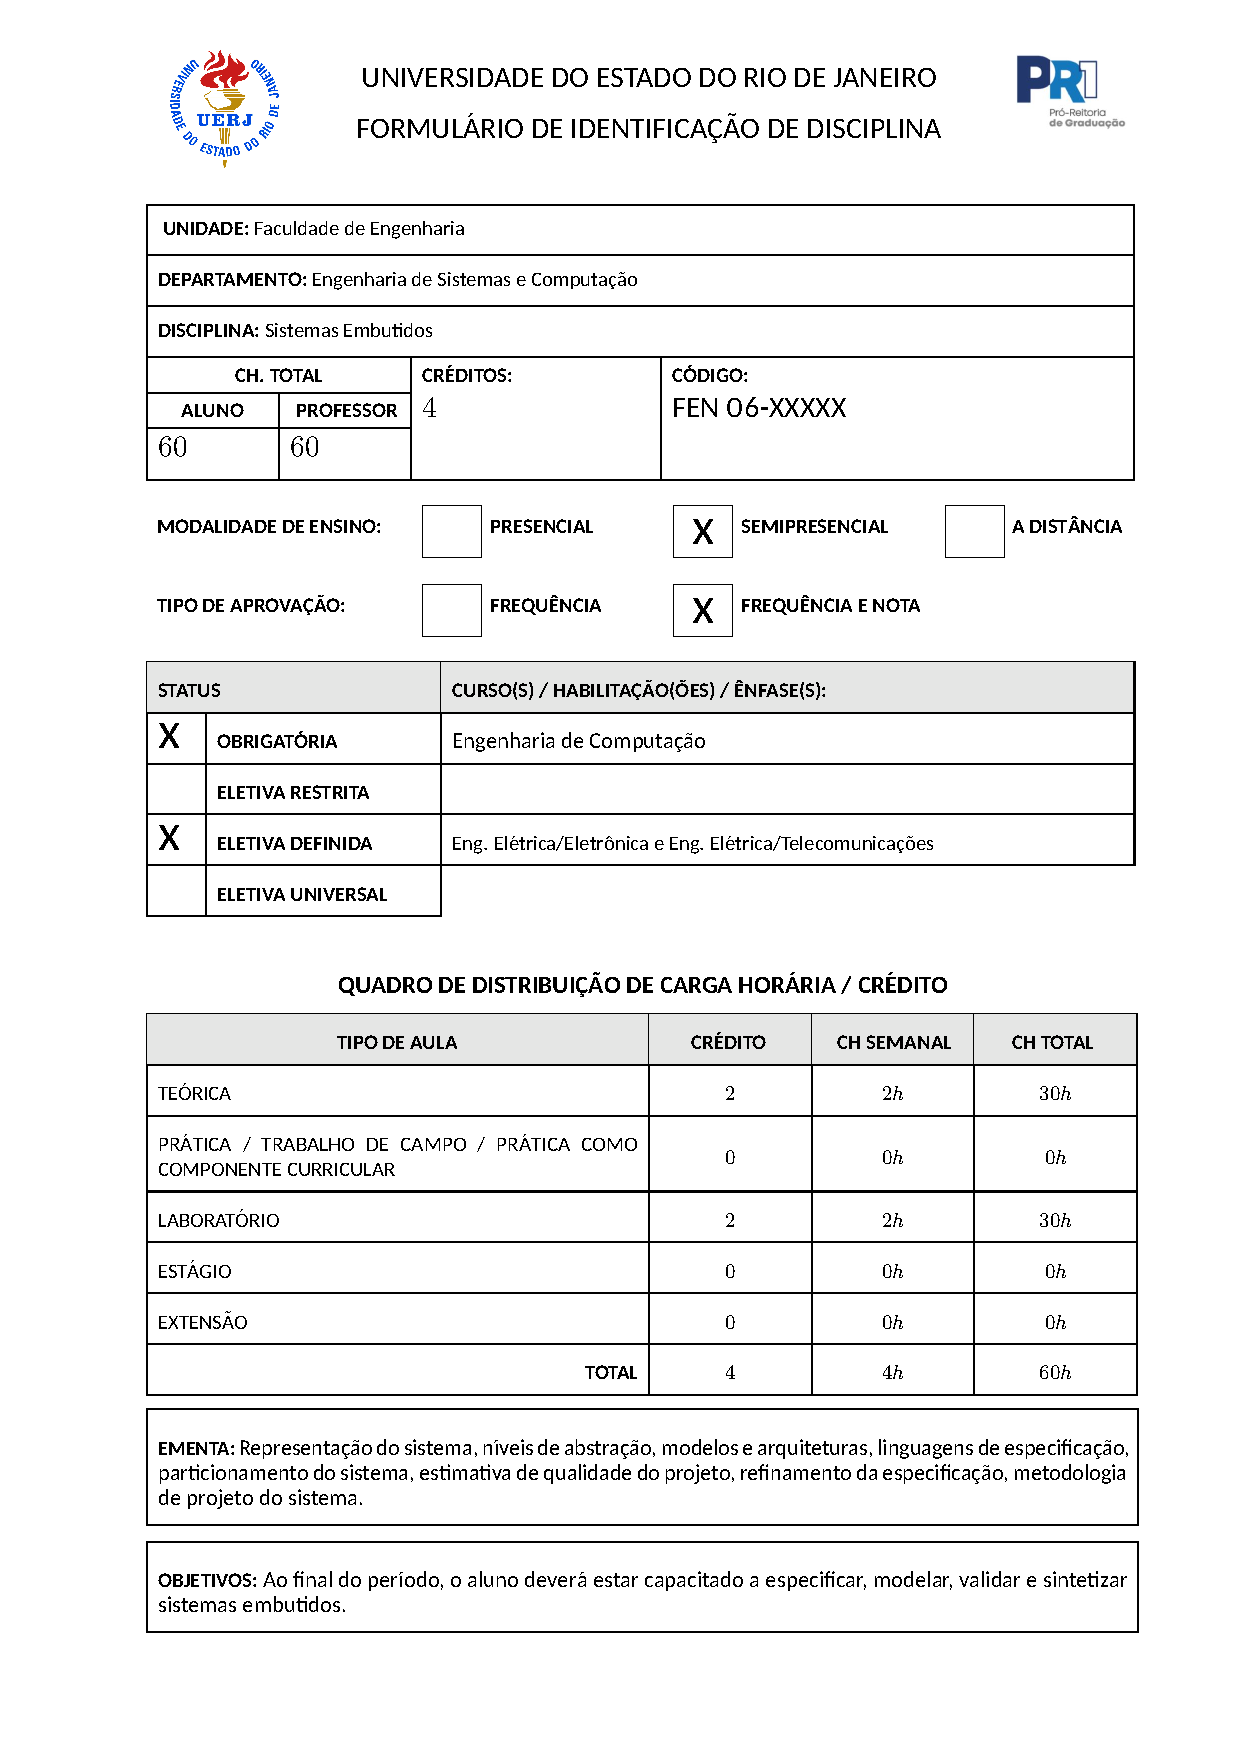
\includepdf[pages=-,addtotoc={1,section,1,{\SistEmb},},pagecommand={\thispagestyle{fancy}}]{ementas/SistemasEmbutidos.pdf}
% Técnicas Digitais
\includepdf[pages=-,addtotoc={1,section,1,{\TeoComp},},pagecommand={\thispagestyle{fancy}}]{ementas/TeoriaDeCompiladores.pdf}
\includepdf[pages=-,addtotoc={1,section,1,{\Grafos},},pagecommand={\thispagestyle{fancy}}]{ementas/TeoriadosGrafos.pdf}


\chapter{Ementas de Disciplinas Eletivas}
% \includepdf[pages=-,addtotoc={1,section,1,{\EletRec},},pagecommand={\thispagestyle{fancy}}]{Eletiva1_ReconhecimentoDePadroes.pdf}
% Aprendizado por Reforço
\includepdf[pages=-,addtotoc={1,section,1,{\EletReforco},},pagecommand={\thispagestyle{fancy}}]{ementas/eletiva_aprendizado_por_reforco.pdf}
% Processamento de Linguagem Natural
\includepdf[pages=-,addtotoc={1,section,1,{\AprendProfPLN},},pagecommand={\thispagestyle{fancy}}]{ementas/eletiva_NLP.pdf}
% Aprendizado Profundo para Visão Computacional
\includepdf[pages=-,addtotoc={1,section,1,{\EletVisao},},pagecommand={\thispagestyle{fancy}}]{ementas/eletiva_visao_computacional.pdf}
% Automação de Processos Robóticos
\includepdf[pages=-,addtotoc={1,section,1,{\AutomProcRob},},pagecommand={\thispagestyle{fancy}}]{ementas/eletiva_automacao_processos_roboticos.pdf}
% Arquiteturas Avançadas de Computadores
\includepdf[pages=-,addtotoc={1,section,1,{\EletArq},},pagecommand={\thispagestyle{fancy}}]{ementas/Eletiva4_ComputacaoDeAltoDesempenho.pdf}
% Geomática
\includepdf[pages=-,addtotoc={1,section,1,{\EletGeo},},pagecommand={\thispagestyle{fancy}}]{ementas/Eletiva3_Geomatica.pdf}
% Redes de Interconexão
\includepdf[pages=-,addtotoc={1,section,1,{\EletRedes},},pagecommand={\thispagestyle{fancy}}]{ementas/Eletiva2_RedesDeInterconexao.pdf}
% Sistemas Operacionais para Robótica Inteligente
\includepdf[pages=-,addtotoc={1,section,1,{\SistOpRobInt},},pagecommand={\thispagestyle{fancy}}]{ementas/eletiva_ROS.pdf}
% Técnicas de Programação em Otimização Combinatória
\includepdf[pages=-,addtotoc={1,section,1,{\TecProgOtim},},pagecommand={\thispagestyle{fancy}}]{ementas/eletiva_tecnicas_de_programacao_em_otimizacao_combinatoria.pdf}
% Tópicos Especiais em Visão Computacional

% Legislação
\includepdf[pages=-,addtotoc={1,section,1,{\TopEspVisComp},},pagecommand={\thispagestyle{fancy}}]{ementas/eletiva_topicos_especiais_em_visao_computacional.pdf}
% Institui as Diretrizes Curriculares Nacionais para os cursos de graduação na área da Computação
\chapter{Resolução CNE/CES n\textordmasculine{} 5, de 16 de novembro de 2016}
\label{cne2016}
\includepdf[pages=-,pagecommand={\thispagestyle{fancy}}]{leis/rces005_16.pdf}
% Referenciais SBC para cursos de Computação
\chapter{SBC: Referenciais para Graduação em Computação}
\label{sbc2017}
\includepdf[pages=-,pagecommand={\thispagestyle{fancy}}]{leis/sbc2017.pdf}
% Resolução CNE/CES n. 7/2018, que estabelece as as Diretrizes para a Extensão na Educação Superior Brasileira
\chapter{RESOLUÇÃO N\textordmasculine{} 7, DE 18 DE DEZEMBRO DE 2018 - CNE/CES}
\label{rcne2018}
\includepdf[pages=-,pagecommand={\thispagestyle{fancy}}]{leis/rces007_18.pdf}
% Deliberação n. 33/95, regras gerais de graduação UERJ
\chapter{Deliberação n\textordmasculine{} 33/95 da UERJ}
\label{delib3395}
\includepdf[pages=-,pagecommand={\thispagestyle{fancy}}]{leis/del-uerj1995.pdf}
% Deliberação n. 59/2019 da UERJ que altera a Deliberação n. 33/95 
\chapter{Deliberação n\textordmasculine{} 59/2019 da UERJ}
\label{delib592019}
\includepdf[pages=-,pagecommand={\thispagestyle{fancy}}]{leis/del-uerj2019.pdf}
%  Resolução n. 380/1993 CREA/CONFEA. Discrimina as atribuições do Engenheiro de Computação
\chapter{Resolução n\textordmasculine{} 380/1993 CREA/CONFEA}
\label{confea1993}
\includepdf[pages=1,pagecommand={\thispagestyle{fancy}}]{leis/confea93.pdf}
% Deliberaçao n. 2/2023 do CSEPE/UERJ dispõe sobre inserção curricular da extensão na UERJ
\chapter{Deliberação n\textordmasculine{} 4/2023 do CSEPE/UERJ}
\label{del4}
\includepdf[pages=-,pagecommand={\thispagestyle{fancy}}]{leis/del-uerj2023.pdf}

\addappheadtotoc

\end{document}
